\documentclass[11pt]{book}
\usepackage[LGR, T1]{fontenc}
\usepackage{textcomp}
\usepackage{fullpage}
%\usepackage{url}
\usepackage{graphicx}
\usepackage{tikz}
\usepackage{tikzsymbols}
\usetikzlibrary{math}
\usetikzlibrary{patterns}
\usepackage{amsmath}
\usepackage{amssymb}
\usepackage{amsthm}
\usepackage[polutonikogreek, french]{babel}
\usepackage{fancyvrb}
\usepackage{lscape}
\usepackage{textcomp}
\usepackage[euler]{textgreek}
\usepackage{lmodern}
\usepackage{alltt}
\usepackage{multirow}
\usepackage{float}
\usepackage[utf8]{inputenc}
\usepackage{ucs}
\usepackage{mflogo}
\usepackage{wrapfig}
\usepackage{proof}
\usepackage[euler]{textgreek}
\usepackage{microtype}
\usepackage[backend=biber]{biblatex}
\usepackage{coqdoc}
\usepackage[nottoc]{tocbibind}

\fvset{tabsize=2}
\newfont{\letterimp}{beta}
\newcommand{\imp}{{\letterimp D}\hspace{0.1cm}}
\newfont{\lettersnow}{snow}
\newcommand{\snow}{{\lettersnow S\hspace{0.2cm}}}
\newcommand{\trans}{\overset{*}{\longrightarrow_{\beta}}}

\title{Le calcul par la réduction et la résolution \\
       Le raisonnement par la preuve et le programme \\

	 Exemples en \textsc{Scheme}, \textsc{Ocaml}, \textsc{Coq} et \textsc{Agda}\\ \vspace{1cm}
   \textgreek{᾿Αγεωμέτρητος μηδε εἰσίτω} \\
      }

\author{Vincent Cognet}
\date{Sainte-Marguerite, le 27 avril 2020 \\
      \url{https://github.com/cogtoto}}

\newtheorem{definition}{Définition}
\newtheorem{theoreme}{Théorème}

\addbibresource{book.bib}  
\begin{document}
\maketitle
\tableofcontents

\chapter{\textgreek{Ἐν ἀρχή}, Gn 1.1 et Jn 1.1}

\textit{Aristote considérait les mathématiques comme une discipline, non pas tant de la vérité, que de la beauté.}
\cite{ab}

\textit{What is mathematics ? Mathematics as an expression of the human mind reflects
the active will, the contemplative reason, and the desire for aesthetic perfection.} \cite{wm}

C'est sous cet angle de l'esthétique que je décrirai ici quelques concepts des fondements 
mathématiques\footnote{\textgreek{\textbf{manj'anw}} : \textit{j'apprends} 
\textgreek{\textbf{t`o m'ajhma}} : \textit{l'étude} 
\textgreek{\textbf{t`a majhmatik'a}} : \textit{les mathématiques, l'étude par excellence}} de l'informatique. \\

 \vspace{0.5cm}

Qu'est-ce que le \textbf{calcul} ? Il est difficile d'en donner une définition abstraite. Essayons cependant de 
décrire l'action de calculer, le processus du calcul. 

Nous identifions deux processus bien distincts appelés la \textbf{réduction} et la \textbf{résolution}.
La réduction est l'action de réduire séquentiellement une expression en une autre plus simple
au moyen de règles de réécriture. Lorsque plus aucune règle ne s'applique, l'expression calculée
 est alors en forme
\textit{normale}. Cette forme normale correspondra à la \textit{valeur} de notre calcul. \\
$(3+8)+(4-9)*2$ \,\imp\,  $11 -5*2$ \, \imp\, $11 -10$ \,\imp\, $1$ \\

Ce processus de réduction soulève deux difficultés essentielles : 
\begin{itemize}
	\item La terminaison. Est-ce-que le processus termine en un nombre fini d'étapes ?
	\item La confluence. Si le processus termine, est-ce-que l'expression aboutit à une forme normale unique ?
\end{itemize}
\vspace{0.3cm}
La fonction mathématique usuelle est peu adaptée à une étude du processus du calcul. Car elle
repose en fait sur une définition en \textit{extension} : une fonction mathématique est la 
description d'une relation d'un ensemble de départ face à son ensemble d'arrivée.

Pour modéliser notre processus de calcul, il nous faut une définition en \textit{intension}, 
c'est-à-dire avec des règles de calcul explicites. Fondé sur
cette idée, le $\lambda$-calcul a été créé par Alonzo Church dans les années 1930.
Il est maintenant utilisé comme socle de tout langage fonctionnel. 
Même s'il est  rudimentaire et basé sur un mécanisme simple de réécriture,
nous verrons qu'il permet d'exprimer toutes les fonctions calculables. Sa \textit{puissance}
de calcul est similaire aux machines de Turing ou aux fonctions $\mu$-récursives de Gödel.
Nous l'étudierons en détails.

\vspace{0.3cm}
L'autre processus de calcul est la résolution. Nous l'utilisons chaque fois que nous devons résoudre
une équation. En résolvant $x^2+2x-15=0$, nous souhaitons que notre processus 
soit \textit{complet}, c'est-à-dire que nous calculions 
l'ensemble des valeurs possibles $\{-5; 3\}$.
 Nous étudierons également  ce mécanisme, et en particulier l'algorithme d'unification.

\vspace{0.3cm}
Enfin, nous aborderons la correspondance bluffante de la programmation fonctionnelle avec la logique. 
C'est la correspondance de Curry-Howard. \\
Avec un langage de programmation typé comme \textsc{Ocaml} où tout terme a un type, nous pouvons
considérer un terme comme étant  la preuve (ou plutôt une des preuves possibles) de son type. 
Le mécanisme strict de typage nous assure de la cohérence du terme avec son type.
Nous avons alors le rapprochement suivant : 

\begin{center}
\begin{tabular}[]{|c|c|}
  \hline
  terme & preuve \\
  \hline
  type & proposition \\
  \hline
\end{tabular}

\end{center}
Nous sommes ici dans une logique constructive, démontrer une proposition revient à exhiber une preuve, c'est-à-dire 
un terme ayant pour type la proposition.
Ainsi, le principe du tiers-exclus $P \vee  \neg P$ ne peut être ici démontré.

Le type faux est un type inhabité, donc nous le définissons sans constructeur : \verb+ type faux = | +

Nous pouvons par exemple prouver le théorème du modus tollens : \\

\verb+let modus_tollens (hfq:'q->faux) (hpq:'p->'q) (hp:'p) = hfq (hpq hp)+  \\
Le type de cette expression est  \verb+('q -> faux) -> ('p -> 'q) -> 'p -> faux+  \\

Dans un langage proposant un système de types plus évolué comme \textsc{Coq}, le faux peut être exprimé 
par le type $\forall p:P, p$. Ce type est également inhabité. Supposer le faux permettra de démontrer 
n'importe quelle proposition.

\begin{Verbatim}
Theorem faux : forall P:Prop, P.
Admitted.

Theorem absurdité : 1=2.
Proof.
    exact (faux (1=2)). 
Qed.
\end{Verbatim}

La correspondance de Curry-Howard montre toute son étendue dans le calcul des constructions, qui 
considère les types comme des termes de premier ordre et permet ainsi de modéliser des types dépendants.
\textsc{Coq} et \textsc{Agda} implémentent ce formalisme.

Nous en montrerons plusieurs exemples significatifs avec ces langages.
Ces exemples nous permettront, je l'espère, de mettre en évidence la frontière entre le calcul et
le raisonnement.

\vspace{0.3cm}
Bonne lecture !

%%%%%%%%%%%%%%%%%%%%%%%%%%%%%%%%%%%%%%%%%%%%%%%%%%%%%%%%%%%%%%%%%%%%%%%%%%%%%%%%%%%%%%%%%%%%%%%%%
%% Le lambda-calcul et la réduction
%%%%%%%%%%%%%%%%%%%%%%%%%%%%%%%%%%%%%%%%%%%%%%%%%%%%%%%%%%%%%%%%%%%%%%%%%%%%%%%%%%%%%%%%%%%%%%%%%
\chapter{Le $\lambda$-calcul et la réduction}

\section{Définition, champ lexical et syntaxique}
Le $\lambda$-calcul est un système formel très rudimentaire. Il n'utilise que  
peu de moyens : le symbole $\lambda$, des variables et des parenthèses. Il n'a
qu'une seule règle de calcul, la $\beta$-réduction, qui modélise le passage d'un
argument à une fonction.

\begin{definition}
Un $\lambda $-terme est défini par induction de la manière suivante:
\begin{itemize}
  \item Une  variable $x$ est un $\lambda$-terme.
  \item Si $t$ est un $\lambda$-terme, l'abstraction $\lambda x.t$ est un $\lambda$-terme.
  \item Si $t_1$ et $t_2$ sont des $\lambda$-termes, l'application $(t_1 \ t_2)$ est un $\lambda$-terme.
\end{itemize}
\end{definition}

Voici le champ lexical des $\lambda $-termes:

\vspace{0.2cm}
token = \begin{tabular}{lll}
| & $\lambda$  & 	{ \verb+LAMBDA+ } \\
| & '.' &  { \verb+POINT+ } \\
| & $[ a-z ] [ a-z\  0-9 ]$ * & { \verb+VARIABLE+ } \\
| & '('	 &	{ \verb+PARLEFT+ } \\
| & ')'	 &	{ \verb+PARRIGHT+ }
\end{tabular}
\vspace{0.4cm}

Voici la grammaire des $\lambda $-termes, en utilisant les terminaux définis
avant :

\vspace{0.2cm}
\begin{tabular}{lll}
\textit{terme} ::= & | & \verb+VARIABLE+  \\
& | & \verb+PARLEFT+ \ \textit{terme} \ \textit{terme} \ \verb+PARRIGHT+ \\
& |& \verb+LAMBDA+ \ \verb+VARIABLE+ \  . \ \textit{terme}
\end{tabular}
\vspace{0.2cm}

Nous utiliserons ocamllex et menhir, qui est la version moderne de ocamlyacc, pour l'analyse lexical et syntaxique des termes
du $\lambda $-calcul.

\subsection{Analyse lexicale avec ocamllex}
Nous d\'{e}finissons ici le champ lexical des diff\'{e}rents \textit{tokens}  (\textit{l\'{e}x\`{e}mes}) du
$\lambda$-calcul.


\begin{Verbatim}
(* file: lambdalexical.mll *)
{
open Lambdagrammar (* Assumes the parser file is "lambdagrammar.mly" *)
}
let texte = ['a'-'z'] ['a'-'z' '0'-'9']*
rule token = parse
| "lambda"	{ LAMBDA }
| '.' { POINT }
| texte as varia	{ VARIABLE (varia) }
| '('		{ PARLEFT }
| ')'		{ PARRIGHT }
| _			{ token lexbuf }
| eof		{ raise End_of_file }
\end{Verbatim}

La compilation de ce fichier \verb+.mll+ va générer une fonction dont le nom
est celui de la règle (ici \verb+token+).
Cette fonction prend comme argument le type \verb+lexbuf+ et rend le type \verb+token+. 

\verb+lexbuf+  est un type de données abstrait défini dans le module Lexing 
qui permet de mémoriser la chaîne ou le fichier en cours d'analyse.
\begin{Verbatim}
val token :  Lexing.lexbuf  -> token 
\end{Verbatim}

\subsection{Analyse syntaxique avec menhir}
Nous d\'{e}finissons ici la grammaire du $\lambda$-calcul.
Nous retrouvons les constructeurs du type ML associ\'{e}s \`{a} chacune des r\`{e}gles de la grammaire.
Ces constructeurs seront préenté dans la section qui suit.


\begin{Verbatim}
/* file: lambdagrammar.mly */
%{
open Terme
%}

%token <string> VARIABLE
%token LAMBDA PARLEFT PARRIGHT POINT
%token NEWLINE

%start exp
%type <Terme.terme> exp

%% /* Grammar rules and actions follow */
exp:      VARIABLE	{ Var($1) }
| PARLEFT exp exp PARRIGHT		{ App($2, $3)}
| LAMBDA VARIABLE POINT exp		{ Lam($2, $4) }
;
%%
\end{Verbatim}



Plus exactement, nous avons modifié cette grammaire \textit{naïve} pour la
rendre non ambiguë et assurer l'associativité à gauche des
$\lambda$-applications.
En effet: 
$$ M N O P = (((M N) O) P) $$
\begin{Verbatim}
%% 
line:  exp NEWLINE { $1 }
;

exp: LAMBDA VARIABLE POINT exp		{ Lam($2, $4) }
		 | app {$1}
;

app:  atome {$1}
		 | app atome { App($1, $2) }
;

atome: PARLEFT exp PARRIGHT {$2}
       | VARIABLE {Var($1)}
;		
%%
\end{Verbatim}
Nous obtenons ainsi:
\begin{Verbatim}
$ ./lambda.out
>> m n o p
App(App(App(Var "m" ,Var "n" ),Var "o" ),Var "p" )

>> lambda f . (lambda x . f(x x)) (lambda x. f(x x))
Lam("f",App(Lam("x",App(Var "f" ,App(Var "x" ,Var "x" ))),
				Lam("x",App(Var "f" ,App(Var "x" ,Var "x" )))))
\end{Verbatim}



La compilation de ce fichier \verb+.mly+ va générer une fonction dont le nom
est celui de l'axiome de notre grammaire (ici \verb+exp+). Cette fonction prend deux arguments: la fonction de l'analyseur lexical qui génère les tokens et l'input. Elle rend le type
des expressions utilisées commes actions dans la grammaire.
\begin{Verbatim}
val exp :   (Lexing.lexbuf  -> token) -> Lexing.lexbuf -> Terme.terme
\end{Verbatim}

 Si le langage analysé n'est pas reconnu par la grammaire, l'exception \verb+Parse_error+ est levée.
 \subsection{Implémentation du parsing en mode \textit{récursif descendant}}
 
 Si nous voulons nous passer d'un outil tel que ocamlyacc ou menhir, nous pouvons très facilement implémenter un parser
 de manière récursive en partant depuis la racine (l'axiome des règles de notre grammaire) et en appelant de manière récursive les
 régles suivantes en fonction du caractère lu.
 
 On modifiera légèrement la grammaire comme ci-dessous pour faciliter le travail.
 
 
\vspace{0.5cm}
\begin{tabular}{lll}
\textit{exprule} & $::=$ & | \verb+VARIABLE+  \\
					  &	    & | \verb+PARLEFT+ \  \textit{parrule} \\
					  & 		 & | \verb+NEWLINE+ \\
\textit{parrule} & $::=$ & | \verb+LAMBDA+ \ \textit{lambdarule}  \\
					  &       & | \textit{apprule} \\ 
\textit{lambdarule} & $::=$ & \verb+VARIABLE+  \verb+POINT+  \textit{exprule}  \verb+PARRIGHT+ \\
\textit{apprule} & $::=$    &  \textit{exprule} \textit{exprule}  \verb+PARRIGHT+ \\
\end{tabular}
\vspace{0.5cm}

Cela imposera cependant la saisie systématique des $\lambda$-termes avec des parenthèses autour des abstractions et des applications.
De même, nous n'aurons plus la facilité syntaxique de l'associativité à gauche des applications et de l'associativité à droite
du corps des abstractions.
Je ne sais pas si une telle grammaire peut être conçue pour une analyse en mode
récursif descendant.
Je pense que non (après m'être un peu cassé les cheveux là-dessus... ). 

Voici le code associé.
\begin{Verbatim}
exception Fin
exception Erreur of string
	
let _ =
	let lexbuf = Lexing.from_channel stdin in
				
	let rec exprule courant =
		match courant with
		| VARIABLE(x) -> Var(x)
		| PARLEFT -> parrule (lexana lexbuf)
		| NEWLINE -> raise Fin
		| _ ->  raise (Erreur "exprule")
		
		and parrule courant =
			  match courant with
				| LAMBDA -> lambdarule courant
				| _ -> apprule courant
		 
		and apprule courant =
				let op1 = exprule courant in
			   let op2 = exprule (lexana lexbuf) in
				let suivant = lexana lexbuf in (* consume PARRIGHT*)
				match suivant with 
					| PARRIGHT ->  App(op1, op2) 
					| _ -> raise (Erreur "apprule")
		 
		and lambdarule courant =
			  let var = lexana lexbuf in 
				let _ = lexana lexbuf in  (* consume POINT *)
				let corps = exprule(lexana lexbuf) in
				let _ =  lexana lexbuf (* consume PARRIGHT *) in
				match var with 
					| VARIABLE(x) -> Lam(x, corps)
					| _ -> raise (Erreur "lambdarule")
			
		in (betaNormalPrint (exprule (lexana lexbuf)); flush stdout)
\end{Verbatim}

\section{Représentation en \textsc{Ocaml}}

\begin{Verbatim}
type terme =
| Var of string
| App of terme * terme
| Lam of variable * terme
\end{Verbatim}


Un terme du $\lambda $-calcul est donc un type ML compos\'{e}, avec les constructeurs $Var$, $App$ et $Lam$.

Par exemple, le terme $ \lambda x.(x y) z $ est represent\'{e} par la structure:



\verb+App ((Lam ("x", (App ((Var "x"), (Var "y"))))), (Var "z"))+


C'est un peu verbeux.
Voici cependant sa représentation sous la forme d'un arbre syntaxique. Le symbole @ repr\'{e}sente ici l'application.
\begin{center}
\begin{tikzpicture}[level distance=1.5cm,
level 1/.style={sibling distance=3cm},
level 2/.style={sibling distance=1.5cm}, scale=0.7]
\node{@}
child { node {$\lambda $}
		child { node {x} }
		child { node {@}
				child { node {x} }
				child { node {y} }
			  }
	  }
child { node {z} };
\end{tikzpicture}
\end{center}

Pour dessiner cet arbre, nous utilisons le tr\`{e}s bon package \textsc{Tikz} qui permet facilement de repr\'{e}senter
les arbres avec une syntaxe très simple.
\begin{Verbatim}
\node{@}
child { node {$\lambda $}
		child { node {x} }
		child { node {@}
				child { node {x} }
				child { node {y} }
			  }
	  }
child { node {z} };
\end{Verbatim}

On impl\'{e}mente deux fonctions \textsc{Ocaml}
qui permettent  d'afficher une expression de type $\lambda $-terme en code \LaTeX\ ou en code \textsc{Tikz}.



La fonction \verb+varLibres+ retourne les variables libres (ie. non li\'{e}es) d'un $\lambda $-terme.
\begin{Verbatim}
let rec varLibres lambdaTerm =
	match lambdaTerm with
	| Var x -> [ x ]
	| App (n, m) -> union (varLibres n) (varLibres m)
	| Lam (x, m) -> remove x (varLibres m)
\end{Verbatim}


Par exemple: $(\lambda x.yxw)(\lambda u.uv) \longmapsto  y,w,v $

\begin{Verbatim}
let exemple = App (Lam ("x", App (Var("y"), App (Var("x"),Var("w")))),
Lam ("u", App (Var ("u"), Var ("v")))) ;;
varLibres exemple ;;
- : variable list = ["y"; "w"; "v"]
\end{Verbatim}


\begin{definition}
Un redex ou radical est un terme de la forme $(\lambda x.M)N$
\end{definition}
On a déjà distingué deux formes possible sur les $\lambda$-termes : les \textit{abstractions} $\lambda x.M$ et les
\textit{applications} $(M N)$. Un \textit{redex} qui est de la forme $(\lambda x.M)N$ est la
rencontre d'une abstraction et d'une application. Voici son implémentation.


\vspace{0.5cm}
\begin{center}
\begin{tabular}{c | c} \hline
ML & SCHEME \\ \hline
\texttt{(function x -> M) N} &  \texttt{((lambda (x) M) N)} \\ 
\texttt{let x = N in M} & \texttt{(let ((x N)) M)} \\ 
\texttt{M where x = N} &  \\ 
\end{tabular}
\end{center}
La dernière syntaxe \texttt{M where x = N} a disparu en \textsc{Ocaml}. C'est dommage car elle est très élégante.
Nous essayerons de la reprendre pour notre interprète maison \textsc{MiniML}.

\begin{definition}
La $\beta $-r\'{e}duction est une op\'{e}ration de substitution. Elle consiste \`{a} substituer dans le redex
$(\lambda x.M) N$ les occurrences libres de x dans M par l'argument N.
On la formalise par la notation suivante:
$$
((\lambda x.M) N) \rightarrow _\beta M[x \leftarrow N]
$$
\end{definition}



Nous pouvons la décrire par les quatre règles d'inférence ci-dessous:
$$
\mathbf{(redex)} : \frac{}{((\lambda x.M)N) \rightarrow M[x \leftarrow N]} \\
$$
$$
\mathbf{(abstraction)} : \frac{M \rightarrow M_1}{ \lambda x.M \rightarrow (\lambda x.M_1)}
\quad \mathbf{(1)} : \frac{M \rightarrow M_1}{(M N) \rightarrow (M_1 N)}
\quad \mathbf{(2)} : \frac{N \rightarrow N_1}{(M N) \rightarrow (M N_1)}
$$

\vspace{0.5cm}
Pour l'implémentation, nous nous sommes appuyés sur le code de l'excellent livre \textit{Programmer avec Scheme} 
de Jacques Chazarain \cite{plisp}.  
Nous avons adapté son code \textsc{Scheme} en \textsc{Ocaml}. En comparant les deux versions, on s'aperçoit finalement
que la version \textsc{Ocaml}, même si un peu plus concise que la version \textsc{Scheme} grâce  l'utilisation du \textit{pattern matching},
reste très proche de l'original \textsc{Scheme}.

\vspace{0.5cm}
La fonction \texttt{substituer} permet de substituer la variable \texttt{var} par le terme \texttt{terme} dans l'expression \texttt{exp}.

\begin{Verbatim}
let rec substituer exp var terme =
	match exp with
	| Var x -> if x = var then terme else exp
	| App (n, m) -> App ((substituer n var terme), (substituer m var terme))
	| Lam (x, m) -> (* pas d'occurence libre on en fait rien *)
			if not (mem var (varLibres exp))
			then exp
			else (* si capture on renome *)
			if mem x (varLibres terme)
			then
				(let newV = renomme x (varLibres terme) in
					let newCorps = substituer m x (Var newV)
					in Lam (newV, (substituer newCorps var terme)))
			else  Lam (x, (substituer m var terme))
\end{Verbatim}

Avant de substituer une variable par une autre, nous devons nous assurer qu'il n'y aura pas de phénomène de capture, ie.
nous assurer qu'une variable libre ne deviendra pas liée, après substitution.
Dans l'exemple suivant, la variable x qui était libre dans $ (z x) $ se retrouve capturée par la lambda.
$$ \lambda x. (x y)[y \gets (z x)] = \lambda x.(x (z x)) $$
Pour éviter cela, il faut avant substitution opérer un renommage de la variable liée:
$$ \lambda x_1. (x_1 y)[y \gets (z x)] = \lambda x_1.(x_1 (z x)) $$
Ce renommage est appelé $\alpha$-conversion. On dit que deux termes $M$ et $N$ sont équivalents modulo $\alpha$.
On écrira $M=_\alpha N$

\begin{Verbatim}
(** renommer var *)
let renomme var listeVar =
	let rec renommeAux j =
		let varj = var ^ (string_of_int j)
		in if mem varj listeVar then renommeAux (j + 1) else varj
	in renommeAux 0
\end{Verbatim}

La fonction \texttt{reduc1Normale}  r\'{e}duit le terme en appliquant la strat\'{e}gie de r\'{e}duction normale, c'est-\`{a}-dire
en commencant la r\'{e}duction par le redex ext\`{e}rieur, plus pr\'{e}cis\'{e}ment le plus \`{a} gauche des ext\`{e}rieurs.



\begin{Verbatim}
let rec reduc1Normale terme =
   match terme with
   | Var x -> raise IRREDUCTIBLE 
   | Lam (x, m) -> Lam (x, (reduc1Normale m))
   | App (n, m) ->
	 if estRedex terme
		then betaReducRedex terme
		else
			try App ((reduc1Normale n), m)
			with IRREDUCTIBLE   -> App (n, (reduc1Normale m)) 
\end{Verbatim}

Enfin, nous avons une fonction \verb+fullReduc+ qui permet d'itérer l'opération de
$\beta$-réduction jusqu'à trouver la forme normale, ou boucler s'il n'y a pas de forme formale.
On lui impose donc maximum 1000 réductions. 
Elle prend en argument la méthode (ie. la stratégie de réduction) à  utiliser. 

\begin{Verbatim}
let rec fullReduc terme methode  =
  let rec loop terme  iter =
	try
	 let newterme = methode terme in
		if (newterme = terme || iter = 0) then newterme
		else loop newterme (iter - 1)
	with IRREDUCTIBLE -> terme	
  in loop terme 1000
	
let betaNormal t = fullReduc t reduc1Normale
\end{Verbatim}

\begin{theoreme}
La réduction normale appliquée à un terme normalisable aboutit toujours à la forme irréductible du terme.
\end{theoreme}

Nous avons en plus le théorème suivant (plus précisément son corollaire) qui nous assure que toutes les réductions d'un $\lambda$-terme (qui terminent) aboutissent au m\^{e}me
terme irréductible.



\begin{theoreme}
Théorème de Church-Rosser : la $\beta $-réduction est confluente.
\end{theoreme}
\begin{tikzpicture}
	\draw [-latex] (1,1) node[above]{$M$} --node{$*$}   (0,0) node[left]{$M_1$} ;
	\draw [-latex] (1,1) --node{$*$}  (2,0) node[right]{$M_2$};
	\draw [-latex, dotted] (0,0) --node{$*$}  (1,-1) node[below] {$M'$};
	\draw [-latex, dotted] (2,0) --node{$*$}  (1,-1) ; 
	\node [text width = 9cm] at(8,0)  {si $M \overset{*}{\longrightarrow_{\beta}} M_1$ et $M \overset{*}{\longrightarrow_{\beta}}  M_2$ alors 
	$\exists\, M'$ tel que  $M_1 \overset{*}{\longrightarrow_{\beta}}  M'$ et $M_2 \overset{*}{\longrightarrow_{\beta}}  M'$} ;
\end{tikzpicture}

\begin{theoreme}
	Corollaire du théorème de Church-Rosser \\
	Si $M$ est normalisable, il existe un unique terme normal, noté $\overline{M}$ tel 
	que $M \overset{*}{\longrightarrow_{\beta}} \overline{M}$
\end{theoreme}
Un corollaire ne devrait pas nécessiter de preuve car supposée évidente. La voici cependant:

\begin{tikzpicture}
	\draw [-latex] (1,1) node[above]{$M$} --node{$*$}   (0,0) node[left]{$M_1$} ;
	\draw [-latex] (1,1) --node{$*$}  (2,0) node[right]{$M_2$};
	\draw [-latex, dotted] (0,0) --node{$*$} node[below left, sloped, midway]{$=$} (1,-1) node[below] {$M3$};
	\node at(1,0) {$=$} ; 
	\draw [-latex, dotted] (2,0) --node{$*$} node[below right, sloped, midway]{$=$} (1,-1) ; 
	\node [text width = 12cm] at(10,0)	{ Si $M$ est normalisable, alors il existe $M_1$ normal
	tel que $M \trans M_1$ ; si $M \trans M_2$ avec
	$M_2$ normal, alors par confluence il existe $M_3$ tel que $M1 \trans M_3$ et  $M2 \trans M_3$.
	Or $M_1$ et $M_2$ sont normaux donc $M_1=M_3$ et $M_2=M_3$ donc $M_1 = M_2$ .	
	 }	  ;
\end{tikzpicture}

\begin{Verbatim}
let t1 = App (Lam ("x",App (Lam ("y", App (Var ("x"), Var ("y"))),Var ("u"))), Var ("z")) ;;
# fullReduc t1 ;;
--> ((lambda x . ((lambda y . (xy))u))z)
--> ((lambda y . (zy))u)
--> (zu)
- : unit -> unit = <fun>
\end{Verbatim}
$$ (\lambda x . (\lambda y . xy)u)z   \rightarrow _\beta (\lambda y . zy) u  \rightarrow _\beta (zu)
$$
\begin{center}
\begin{tabular}{|c|c|c|} \hline
$(\lambda x . (\lambda y . xy)u)z$ & $(\lambda y . zy)u$ & $(zu)$ \\ \hline
\mbox{
\begin{tikzpicture}[level distance=1.5cm,
level 1/.style={sibling distance=3cm},
level 2/.style={sibling distance=1.5cm}, scale=0.6]
\node {@} child { node {$\lambda$} child { node{x} } child {node {@} child { node {$\lambda$} child { node{y} }
child {node {@} child { node {x }}  child {node {y }} } }  child {node {u }} } }  child {node {z }} ;
\end{tikzpicture}
}
& \mbox {
\begin{tikzpicture}[level distance=1.5cm,
level 1/.style={sibling distance=3cm},
level 2/.style={sibling distance=1.5cm}, scale=0.6]
\node {@} child { node {$\lambda$} child { node{y} }
child {node {@} child { node {z }}  child {node {y }} } }
child {node {u }} ;
\end{tikzpicture}
}
&
\mbox {
\begin{tikzpicture}[level distance=1.5cm,
level 1/.style={sibling distance=3cm}, scale=0.6 ]
\node {@} child { node {z} }
child { node{u} } ;
\end{tikzpicture}
}
\\ \hline
\end{tabular}
\end{center}

\vspace{1cm}
Voici un exemple de terme qui ne termine pas et qui enfle.
$$ (\lambda x.xxx)(\lambda x.xxx) \rightarrow _\beta (\lambda x.xxx)(\lambda x.xxx)(\lambda x.xxx)
\rightarrow _\beta (\lambda x.xxx)(\lambda x.xxx)(\lambda x.xxx)(\lambda x.xxx) \rightarrow _\beta \ldots
$$  

Nous pouvons programmer facilement en \textsc{Ocaml} le terme $\Omega \equiv \Delta \Delta \equiv (\lambda x.xx)(\lambda x.xx)$
qui n'a pas de forme normale.
\begin{verbatim}
type terme = | Lam : (terme -> terme) -> terme ;;
let app t1 t2 = match t1 with | Lam f -> f t2 ;;
let delta = Lam (fun x -> (app x x)) in app delta delta ;;
\end{verbatim} 


\section{Démonstration de la confluence du $\lambda$-calcul}
Comment prouver que le $\lambda$-calcul est bien confluent ? C'est-à-dire que pour tout terme $M$, si $M\twoheadrightarrow M_1$ et
  $ M\twoheadrightarrow M_2 $,
alors il existe $M_3$ tel que $M_1\twoheadrightarrow M_3$ et  $M_2\twoheadrightarrow  M_3$.

La démonstration pose quelques difficultés techniques.

\begin{enumerate}
	\item Il est difficile de raisonner par cas sur une relation $\twoheadrightarrow $
	 qui est la cloture transitive
	 et réflexive de la réduction en une étape $\rightarrow$

	\item La réduction en une étape $\rightarrow$ n'a pas la propriété du diamant. Nous la rappelons : pour tout terme $M$,
	 si $M\rightarrow  M_1$ et  $M\rightarrow M_2$,
alors il existe $M_3$ tel que $M_1\rightarrow M_3$ et  $M_2\rightarrow M_3$.

En effet, soit $R$ un redex qui se reduit en $R'$, le terme $(\lambda x.xx) R \rightarrow RR$ ou bien 
 $(\lambda x.xx) R \rightarrow (\lambda x.xx) R'$. Il faudra une ou deux étapes pour arriver à $R'R'$. 

 \item On démontre facilement (par étude de cas sur la structure du $\lambda$-terme) 
 la faible confluence de la relation $\beta$, ç-à-d si $M \rightarrow M_1$ et $M \rightarrow M_2$, alors
 il existe $M_3$ tel que $M_1 \twoheadrightarrow M_3$ et $M_2 \twoheadrightarrow M_3$.
 Cependant la confluence faible n'implique pas la confluence si la relation n'est pas noetherienne.
 C'est le cas du lambda calcul qui n'est pas fortement normalisant... 
Considérons $\Omega \equiv (\lambda x.xx) (\lambda x.xx) $, nous avons une chaîne de réduction infinie $\Omega \rightarrow \Omega \rightarrow \dots $

 \item Cependant, nous pourrons démontrer plus facilement la propriété du parallélogramme: pour tout terme $M$,
  si $M\rightarrow M_1$ et  $M\twoheadrightarrow  M_2$,
alors il existe $M_3$ tel que $M_1\twoheadrightarrow  M_3$ et  $M_2\twoheadrightarrow M_3$.

Cette propriété du parallélogramme qui semble plus faible que la confluence lui est en fait équivalente. Cela
s'explique par le diagramme suivant :

\begin{center}
\begin{tikzpicture}[scale=0.5]
	\draw [-latex] (3,3) -- (2,2)  ;
	\draw [-latex] (3,3) --node{$*$} (6,0)  ;
	\draw [-latex] (2,2) --node{$*$} (5,-1)  ;
	\draw [-latex] (6,0) --node{$*$} (5,-1)  ;

	\draw [-latex, dashed] (2,2) -- (1,1) ;
	\draw [dotted] (1,1) -- (0,0) ;
	\draw [-latex, dashed] (0,0) -- (-1,-1) ;

	\draw [-latex, dashed] (1,1) --node{$*$}  (4,-2) ;
	\draw [-latex, dashed] (0,0) -- node{$*$} (3,-3) ;
	\draw [-latex, dashed] (-1,-1) -- node{$*$} (2,-4) ;

	\draw [-latex, dashed] (5,-1) -- node{$*$} (4,-2) ;
	\draw [dotted] (4,-2) -- (3,-3) ;
	\draw [-latex, dashed] (3,-3) -- node{$*$} (2,-4) ;
\end{tikzpicture}
\end{center}

\item L'idée de la démonstration est simple : supposons $M \stackrel{\Delta}{\rightarrow} M_1  $ où
$\Delta$ est un redex de $M$. Si dans la réduction $M\twoheadrightarrow M_2$, on garde la trace de ce qui se passe
sur $\Delta$, alors en réduisant tous les résidus de $M_2$, on obtiendra $M_3$.
\end{enumerate}

\subsection{La restriction $\Lambda '$ du $\lambda$-calcul}
Pour tracer les redex uniquement à réduire, on introduit $\Lambda '$, une restriction du $\lambda$-calcul.


$\Lambda '$ est définie de manière inductive comme ci-dessous comme le $\lambda$-calcul avec en addition
l'expression $((\lambda _i x.M)N)$ pour $i \in \mathbb{N}$
Ainsi, nous marquons par un indice $i$ le redex que nous voulons tracer.
Nous définissons également la réduction $\beta '$  qui contient la réduction $\beta$ et y ajoute 
$(\lambda_i x.M)N \rightarrow M [x:=N]$

Enfin, nous ajoutons la fonction $\phi$ qui réduit uniquement les redex indicés, et non les autres.
$$\phi ((\lambda _i x.P)Q) \equiv \phi (P) [x:=\phi(Q)]$$

Nous utilisons les notations $M\stackrel{\shortparallel }{\longrightarrow} N$
et $M\stackrel{\phi } {\longrightarrow}N$

Le pouvoir réducteur de $\beta '$ est le même que $\beta$.
En outre, on a la propriété suivante : si $M \stackrel{\beta '}{\twoheadrightarrow} N$,
alors   $\phi(M) \stackrel{\beta}{\longrightarrow} \phi (N)$ 

\subsection{La démonstration}
Nous présentons ici la démonstration détaillée dans \cite{baren_bible}.

\begin{enumerate}
	\item Hypothèses: $M\stackrel{\beta}{\twoheadrightarrow} N$ et
                    $M\stackrel{\beta}{\rightarrow} M'$        
       \item Cherchons à prouver qu'il existe $N'$ tel que  $N\stackrel{\beta}{\twoheadrightarrow} N'$ 
et  $M' \stackrel{\beta}{\twoheadrightarrow} N'$ 
        \item $M'$ est le résultat de la contraction du redex $\Delta$ dans $M$. Soit $\tilde{M} \in \Lambda '$
        obtenu de $M$ en indexant $\Delta$. Alors, $ \tilde{M} \stackrel{\shortparallel}{\rightarrow} M$ et 
       $ \tilde{M} \stackrel{\phi}{\rightarrow} M'$ 
       \item Nous obtenons, l'existence d'un $\tilde{N}$ par $\tilde{M}\stackrel{\beta '}\twoheadrightarrow \tilde{N}$
       \item Nous obtenons aussi l'existence d'un $N'$ tel que $\tilde{N} \stackrel{\phi}{\twoheadrightarrow} N'$
       et $N \stackrel{\beta}{\twoheadrightarrow} N'$
       \item Nous avons de même $M' \stackrel{\beta}{\twoheadrightarrow} N'$
       \item Nous avons bien trouvé notre terme confluent $N'\ \  \square $

\end{enumerate}

\subsection{Un exemple}
\begin{enumerate}
	\item Soit $M \equiv (\lambda x.xx)((\lambda y.z)w)$ , nous avons 
	$M \stackrel{\beta}{\rightarrow} N' \equiv (\lambda x.xx)z$ et $M \stackrel{\beta}{\rightarrow} N \equiv ((\lambda y.z)w)((\lambda y.z)w)$
       \item Cherchons  $N'$ tel que  $N\stackrel{\beta}{\twoheadrightarrow} N'$ 
et  $M' \stackrel{\beta}{\twoheadrightarrow} N'$ 
	\item  Soit le redex $\Delta$ de $M$ tel que $\Delta \equiv ((\lambda y.z)w)$, alors $\tilde{M} \equiv (\lambda x.xx)((\lambda_1 y.z)w)$
	Nous avons $\tilde{M}  \stackrel{\phi}{\rightarrow} M' \equiv (\lambda x.xx)z$
	\item $\tilde{N}$ est obtenu de la même manière que $N$, mais en marquant les résidus de $\Delta$ :
	 $\tilde{N} \equiv  ((\lambda _1 y.z)w)((\lambda _1 y.z)w)$

	 \item  Nous réduisons maintenant les résidus de $\tilde{N}$ pour obtenir
	  $\tilde{N}  \stackrel{\phi}{\twoheadrightarrow} zz$ \\
	  Aussi, nous avons bien également $N \stackrel{\beta}{\twoheadrightarrow} zz$

	 \item Nous avons également $M' \equiv (\lambda x.xx)z \stackrel{\beta}{\rightarrow} zz$
	 \item Ainsi $N' \equiv zz$
\end{enumerate}

\subsection{La $\beta$-réduction parallèle}
Une autre méthode de démonstration de la confluence repose sur l'introduction d'une nouvelle relation $\beta _\parallel $.
Cette relation va permettre la réduction simultanée de plusieurs redex du $\lambda$-terme.

\begin{definition}
	La $\beta _\parallel$ réduction repose sur les 4 règles suivantes:
	\begin{enumerate}
		\item  
		$ x \Rightarrow_\beta  x $
		\item 
		$ \lambda x.M \Rightarrow_\beta  \lambda x.M' , si\ M \Rightarrow_\beta  M' $
		\item 
		$ MN \Rightarrow_\beta  M' N' , \ si\ M  \Rightarrow_\beta  M' 
		                                               \ et\ N  \Rightarrow_\beta  N'$
		\item 
		$ (\lambda x.M)N \Rightarrow_\beta M'[x:=N'] , \ si\ M \Rightarrow_\beta  M' 
		                                               \ et\ N  \Rightarrow_\beta N'$
	\end{enumerate}

\end{definition}
On peut démontrer par induction que cette relation $\beta _\parallel$ respecte la propriété du diamant : si
$M \Rightarrow M_1,M_2$, alors $\exists N$ tel que $M_1,M_2  \Rightarrow N$.

Cependant, nous allons encore plus simplement montrer qu'il existe un $M^*$ tel que si $M  \Rightarrow N  \forall N$, alors
$N  \Rightarrow M^*$. Ce $M^*$ sera indépendant de $N$.
L'idée est que le terme $M^*$ sera obtenu en réduisant simultanément tous les redex présents dans $M$.


Soit la fonction $\mathcal{G}$, tel que 
\begin{align}
	\mathcal{G}(x)&=x \\
	\mathcal{G}(\lambda x.M) &= \lambda x.(\mathcal{G}(M)) \\
	\mathcal{G}(MN)&= \mathcal{G}(M)\mathcal{G}(N), \ si\ M \neq \lambda x.M_1 \\
	 \mathcal{G}((\lambda x.M)N) &= \mathcal{G}(M)[x:=\mathcal{G}(N)]  
\end{align}
Nous pouvons montrer que si $M  \Rightarrow _\beta N, \forall N$, alors
$N  \Rightarrow  _\beta \mathcal{G}(M)$.
Par induction sur la relation $M  \Rightarrow _\beta N$  :
 \begin{enumerate}
	\item si $M \equiv x$, alors $N \equiv x \equiv \mathcal{G}(x)$

	\item si $M \equiv \lambda x.M_1$, alors $N \equiv \lambda x.N_1$, avec $M_1  \Rightarrow _\beta N_1$. 
	Par récurrence, $M_1  \Rightarrow _\beta \mathcal{G}(M_1)$, donc $M  \Rightarrow _\beta \lambda x.\mathcal{G}(M)_1 \equiv
	\mathcal{G(M)}$

	\item si $M\equiv (M_1 M_2)  \Rightarrow _\beta  N $, alors $N \equiv N_1 N_2$ 
	avec $M_1 \Rightarrow _\beta N_1$ et  $M_2 \Rightarrow _\beta N_2$ , alors nous avons
	 $N_1 N_2 \Rightarrow _\beta \mathcal{G}(N_1) \mathcal{G}(N_2) \equiv \mathcal{G}(M)$

	 \item si $M\equiv ((\lambda x.M_1)M_2) \Rightarrow _\beta N$, alors 2 sous-cas à considérer :
	 \subitem 
	      si $N \equiv (\lambda x.N_1)N_2$, alors $N \Rightarrow _\beta \mathcal{G}(M_1)[x:=\mathcal{G}(M_2)] \equiv \mathcal{G}(M)$
	 \subitem 
	      si $N \equiv N_1[x:=N_2]$, alors $N \Rightarrow _\beta \mathcal{G}(M_1)[x:=\mathcal{G}(M_2)] \equiv \mathcal{G}(M)$ 


\end{enumerate}


\section{La $\beta$-réduction faible avec appel par valeur}
Dans un langage fonctionnel comme \textsc{Scheme} ou \textsc{ML}, il est important de noter que contrairement au $\lambda$-calcul, le corps de la lambda n'est pas \'{e}valu\'{e}. 
On parle de $\beta$-réduction faible.  
Autrement dit, la règle suivante n'est pas utilisée:
$$\mathbf{(abstraction)} : \frac{M \rightarrow M_1}{ \lambda x.M \rightarrow (\lambda x.M_1)}$$
Nous pourrons utiliser cette absence d'\'{e}valuation du corps 
des lambda expressions pour geler l'\'{e}valuation de nos expressions : \verb+(delay exp) = (lambda () exp)+ 

L'appel par valeur signifie que les arguments sont évalué en premier. Les règles d'inférence appliquées sont donc dans cet ordre:

$$
\quad \mathbf{(1)} : \frac{N \rightarrow N_1}{(M N) \rightarrow (M N_1)}
\quad \mathbf{(2)} : \frac{M \rightarrow M_1}{(M N) \rightarrow (M_1 N)}
\quad \mathbf{(3)} : \frac{}{((\lambda x.M)N) \rightarrow M[x \leftarrow N]} 
$$

Voici la fonction ML qui implémente cet ordre:
\begin{Verbatim}
let rec reduc1Valeur terme =
  match terme with
  | Var x -> raise IRREDUCTIBLE
  | Lam (x, m) -> raise IRREDUCTIBLE
  | App (n, m) ->
      (try App (n, (reduc1Valeur m))
       with
       | IRREDUCTIBLE ->
           (try App ((reduc1Valeur n), m)
            with
            | IRREDUCTIBLE ->
                (try betaReducRedex terme
                 with | NOTREDEX -> raise IRREDUCTIBLE)))
\end{Verbatim}

Par exemple, nous aurons les réductions successives suivantes: 

\begin{itemize}
\item réduction normale, qui aboutit toujours à la forme irréductibre
$$ (\lambda x.y) ((\lambda x.xx) (\lambda x.xx)) \rightarrow_\beta y $$ 

\item réduction par valeur 
$$
\begin{array}{ccc}
 (\lambda x.y)((\lambda x.xx) (\lambda x.xx)) &  \rightarrow_\beta  & (\lambda x.y)((\lambda x.xx) (\lambda x.xx))\\ 
 & \rightarrow_\beta  & (\lambda x.y)((\lambda x.xx) (\lambda x.xx)) \\
 &\rightarrow_\beta  & (\lambda x.y)((\lambda x.xx) (\lambda x.xx))) \\
 & \rightarrow_\beta  & \ldots \\
\end{array}
$$
\end{itemize}

\section{Récursivité et points fixes} 

What else is a loop but a way of representing an endless process in a finite way?
\cite{god}


\begin{center}
 \begin{tabular}{cc}
	\parbox[c]{0.3\textwidth}{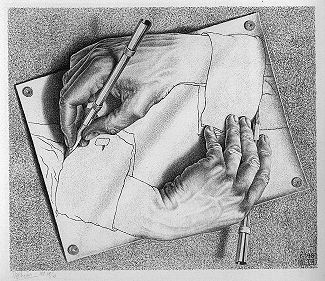
\includegraphics[width=0.3\textwidth]{DrawingHands.jpg}}
  & \hspace{0.5cm}
   $\sqrt{2} = 1 + \frac{1}{1+\sqrt{2}} $  \\
 \end{tabular}
\end{center}

\subsection{Le point fixe du $\lambda$-calcul} %%

En analyse, le point fixe d'une fonction $f$ est sa valeur $x$ telle que $f(x)=x$

Cela permet de d\'{e}finir $x$ en fonction de lui-m\^{e}me.

Cette simple expression $x=f(x)$ est finalement tr\`{e}s \'{e}trange et d\'{e}routante.
C'est la force de la r\'{e}cursivit\'{e} : $x=f(f(f(f(f(f\ldots (x)\ldots))))))$

Un exemple est la valeur $\sqrt{2}$ exprim\'{e}e sous forme d'une fraction continue,
expression trouv\'{e}e je crois par Euler.
Je la d\'{e}cris ci-dessous  pour le plaisir d'\'{e}crire (et lire) de belles formules math\'{e}matiques en \LaTeX
\cite{lamport1994latex}
$$
\sqrt{2} = 1+\sqrt{2} -1
= 1+ \frac{(\sqrt{2} -1)(\sqrt{2} +1)}{\sqrt{2} +1}
= 1 + \frac{1}{1+\sqrt{2}}
$$


\begin{tikzpicture}
	\draw[->] (-1, 0) -- (3, 0) node[right] {$x$};
	\draw[->] (0, -1) -- (0, 3) node[above] {$y$};
	\draw[domain=-0.5:3, smooth, variable=\x, blue] plot (\x, {1 + 1 / (1+ \x) }) node [right] {$y=1 + \frac{1}{1+x} $};
	\draw[domain=-1:3, smooth, variable=\x, red] plot (\x, {\x}) node [right] {$y=x$};
	\draw [dotted] (1.4142,0) node[below]{$\sqrt{2}$}  --(1.4142,1.4142)  ;
	\draw [dotted] (0,1.4142) node[left] {$\sqrt{2}$}  --(1.4142,1.4142) ;
	
	\node [draw,text width=6cm] at(10,1.5) {\[
		\sqrt{2} = 1 + \cfrac{1}{2
		+ \cfrac{1}{2
		+ \cfrac{1}{2
		+ \cfrac{1}{2
		+ \cfrac{1}{ \ddots
		} } } } } \] } ;
\end{tikzpicture} 



En posant $ f(x) = 1 + \frac{1}{1+x} $, la résolution de l'équation $x=f(x)$ nous permet
de calculer la valeur de $\sqrt{2}$. Nous utilisons aussi le fait que $\sqrt{2}$ est 
un point fixe attractif de notre fonction $f$. C'est-à-dire qu'il existe un \textit{voisinage} de 
$\sqrt{2}$ tel que la suite $ x_0,f(x_0),f(f(x_0)),f(f(f(x_0))),\dots $ converge vers $\sqrt{2}$


En \textsc{Ocaml}, la fonction qui it\`{e}re cette fraction continue peut être codée comme suit. 
Nous partons ici de $x_0 =1$. La fraction continue converge très rapidement.
\begin{Verbatim}
let rec square2 iter =
	if (iter = 1) then 1.
	else  1. +. ( 1. /. ( 1. +. square2 (iter - 1)));;
val square2 : int -> float = <fun>

# square2 30 ;;
- : float = 1.4142135623730951

# sqrt 2. ;;
- : float = 1.41421356237309512.

\end{Verbatim}


En $\lambda $-calcul, de manière très surprenante, il s'avère que tout terme a un point fixe !
Nous avons un combinateur\footnote{Un combinateur est un $\lambda$-terme comprenant uniquement 
des variables li\'{e}es} qui nous permet de calculer le point fixe de n'importe quel $\lambda $-terme.
Ce combinateur s'appelle $Y$ . Il est défini par $$ Y=  \lambda f.(\lambda x.f(x x))(\lambda x.f(x x)) $$

Ce n'est pas le seul combinateur de point fixe. Voici un autre d\^{u} \`{a} Turing :
 $$\Theta = (\lambda x. \lambda y. (y (x x y))) (\lambda x. \lambda y. (y (x x y)))$$

Voici l'arbre syntaxique de $Y$:
\begin{center}
\begin{tikzpicture}[level distance=1.5cm,
level 1/.style={sibling distance=5cm},
level 2/.style={sibling distance=3cm},
level 3/.style={sibling distance=1.5cm},
level 4/.style={sibling distance=1.5cm}, scale=0.6]
\node {$\lambda$} child { node{f} } child {node {@} child { node {$\lambda$} child
{ node{x} } child {node {@} child { node {f }}  child {node {@} child { node {x }}
child {node {x }} } } }  child {node {$\lambda$} child { node{x} } child
{node {@} child { node {f }}  child {node {@} child { node {x }}  child {node {x }} } } } } ;
\end{tikzpicture}
\end{center}
Quel que soit le terme $M$, nous aurons  $(YM) = _\beta M(YM)$



Essayons ceci avec notre notre fonction \verb+fullReduc+  en CAML.
Réduisons $YM$ :

$$
\begin{array}{l}
\lambda f . (\lambda x . (f (x x))) (\lambda x . (f (x x))) M \\
\rightarrow _\beta (\lambda x . (M (xx)))(\lambda x . (M(xx))) \\
\rightarrow _\beta  (M(\lambda x . (M(xx)))(\lambda x . (M(xx))))  \triangleright [2] \\
\rightarrow _\beta  (MM(\lambda x . (M(xx)))(\lambda x . (M(xx)))) \\
\rightarrow _\beta  (MMM(\lambda x . (M(xx)))(\lambda x . (M(xx)))) \\
\rightarrow _\beta  (MMMM(\lambda x . (M(xx)))(\lambda x . (M(xx)))) \\
\rightarrow _\beta  \ldots
\end{array}
$$


La deuxième $\beta$-r\'{e}duction est bien \'{e}gale \`{a} $M (Y M)$
Nous voyons ici le mécanisme d'appel récursif à M. 

Détaillons cela avec une fonction exprimée en pseudo-code d'un $\lambda$-calcul étendu.
Nous nous inspirons pour cela du très bon article de wikipedia \url{https://en.wikipedia.org/wiki/Lambda_calculus}.


Soit $M = (\lambda f \lambda n .(if\ n=0\ then\ 1\ else\ n*f(n-1)))$
$$
\begin{array}{lll}
(YM)\ 4 & \rightarrow _\beta & M (YM)\ 4 \\
& \rightarrow _\beta & (\lambda f \lambda n .(if\ n=0\ then\ 1\ else\ n*f(n-1))) (YM)\ 4 \\
& \rightarrow _\beta & (\lambda  n . (if\ n=0\ then\ 1\ else\ n*((YM) (n-1))))\ 4 \\
& \rightarrow _\beta & (if\ 4=0\ then\ 1\ else\ 4*((YM)\ (4-1))) \\
& \rightarrow _\beta & 4 * ((YM)\ 3) \\
& \rightarrow _\beta & 4 * (M(YM)\ 3) \\
& \vdots & \\
& \rightarrow _\beta & 4 * 3 * 2 * 1 
\end{array}
$$

Ici encore, nous avons utilisé la stratégie de $\beta$-réduction normale. 
Mais avec une réduction par valeur, le terme en argument $(YM)$ aura été réduit indéfiniment en $M(M(M(M(M\ldots YM)\ldots)))$,
sans réduire le redex $Mx$


En utilisant notre programme OCAML, voyons cela avec en prenant $M = \lambda a. (\lambda b . b) $ :

\verb+# betaNormal ym ;;+
$$
\begin{array}{lll}
 & (\lambda f . (\lambda x . (f(xx))\lambda x . (f(xx)))\lambda a . \lambda b . b) &  \\
 \rightarrow _\beta & (\lambda x . (\lambda a . \lambda b . b(xx))\lambda x . (\lambda a . \lambda b . b(xx))) &\triangleright [2]  \\
 \rightarrow _\beta & (\lambda a . \lambda b . b(\lambda x . (\lambda a . \lambda b . b(xx))\lambda x . (\lambda a . \lambda b . b(xx))))  &\triangleright [3]  \\
 \rightarrow _\beta & \lambda b . b &  \\
\end{array}
$$

\verb+# betaValeur ym ;;+
$$
\begin{array}{lll}
 & (\lambda f . (\lambda x . (f(xx))\lambda x . (f(xx)))\lambda a . \lambda b . b)  &  \\
\rightarrow _\beta & (\lambda x . (\lambda a . \lambda b . b(xx))\lambda x . (\lambda a . \lambda b . b(xx))) & \triangleright [2]  \\
\rightarrow _\beta & (\lambda a . \lambda b . b(\lambda x . (\lambda a . \lambda b . b(xx))\lambda x . (\lambda a . \lambda b . b(xx)))) & \triangleright [3] \\
\rightarrow _\beta & (\lambda a . \lambda b . b(\lambda a . \lambda b . b(\lambda x . (\lambda a . \lambda b . b(xx))\lambda x . (\lambda a . \lambda b . b(xx)))))  & \\
\rightarrow _\beta & (\lambda a . \lambda b . b(\lambda a . \lambda b . b(\lambda a . \lambda b . b(\lambda x . (\lambda a . \lambda b . b(xx))\lambda x . (\lambda a . \lambda b . b(xx)))))) &  \\
\rightarrow _\beta & (\lambda a . \lambda b . b(\lambda a . \lambda b . b(\lambda a . \lambda b . b(\lambda a . \lambda b . b(\lambda x . (\lambda a . \lambda b . b(xx))\lambda x . (\lambda a . \lambda b . b(xx)))))))  & \\
\end{array}
$$
Les étapes  $\triangleright [2]$ et $\triangleright [3]$ sont bien les mêmes sur les deux stratégies. 
Puis la $\beta$-réduction par valeur va continuer à réduire l'argument
$(YM)$, là où la $\beta$-réduction normale va d'abord réduire le redex $Mx$

Avec la réduction par valeur, il nous faut donc utiliser un autre combinateur de point fixe\footnote{Nous insistons 
là-dessus car nous rappelons que les interprètes \textsc{MiniScheme} et \textsc{MiniML} que nous implémenterons utiliseront la $\beta$-réduction faible par valeur.}
 que nous appelerons $Z$ 
$$Z = \lambda f.(\lambda x.f(\lambda v.xxv))(\lambda x.f(\lambda v.xxv)) $$

On constate que Z est  $\eta$-équivalent à $Y$. Nous rappelons la définition suivante:


\begin{definition}
	
Les termes $(\lambda x.Mx)$ et M sont $\eta$-équivalents. On écrira $(\lambda x.Mx) =_\eta M$

En ML, nous pouvons par exemple dire que \verb+ let g x = f x+ est $\eta$-équivalent à \verb+ let g = f+
\end{definition}


Appliquons à nouveau notre exemple avec ce combinateur $Z$ appliqué à $M=\lambda a. \lambda b. b$:

\verb+# betaValeur zm ;;+
$$
\begin{array}{ll}
& ((\lambda f . ((\lambda x . (f(\lambda v . ((xx)v))))(\lambda x . (f(\lambda v . ((xx)v))))))(\lambda a . (\lambda b . b))) \\
\rightarrow _\beta &  ((\lambda x . ((\lambda a . (\lambda b . b))(\lambda v . ((xx)v))))(\lambda x . ((\lambda a . (\lambda b . b))(\lambda v . ((xx)v))))) \\
\rightarrow _\beta &  ((\lambda a . (\lambda b . b))(\lambda v . (((\lambda x . ((\lambda a . (\lambda b . b))(\lambda v . ((xx)v))))(\lambda x . ((\lambda a . (\lambda b . b))(\lambda v . ((xx)v)))))v))) \\
\rightarrow _\beta &  (\lambda b . b)
\end{array}
$$

Nous avons le même réultat et les même étapes de réduction avec \verb+betaNormal zm ;;+


En SCHEME, nous pourrons implémenter ce combinateur $Z$ :
\begin{Verbatim}
(define Z
 (lambda(f)
   (lambda (x) (lambda(v) ((f (x x) v))))
   (lambda (x) (lambda(v) ((f (x x) v))))))
\end{Verbatim}

En ML, le typage ne nous permettra pas de coder un combinateur comme $Y$ ou $Z$.

Essayons cependant d'écrire:

\begin{Verbatim}

# let rec fix f = f (fix f) ;;
val fix : ('a -> 'a) -> 'a = <fun>

let factabs fact = function
  | 0 -> 1
  | n -> n * fact (n - 1) ;;

val factabs : (int -> int) -> int -> int = <fun>
# (fix factabs) 5 ;;
Stack overflow during evaluation (looping recursion?).
\end{Verbatim}
ML est bien un langage \textit{strict}: les arguments d'une fonction sont évalués en premier 
comme on l'a vu dans la $\beta$-réduction faible avec appel par valeur.


Pour éviter la boucle infinie $f(f\ldots(f (fix f))\ldots)$, 
une astuce que j'ai pu lire est d'introduire une variable supplémentaire:

\begin{Verbatim}
# let rec fix f x = f (fix f) x ;;
val fix : (('a -> 'b) -> 'a -> 'b) -> 'a -> 'b = <fun>
# (fix factabs) 5 ;;
- : int = 120
\end{Verbatim}
Ici aussi, le mécanisme de la ``$\eta$-expansion'' est utilisé.
Reproduisons cela en SCHEME :
\begin{Verbatim}
(define factabs
  (lambda (f)
    (lambda (n)
      (if (eq? n 0)
          1
          (* n (f (- n 1)))))))

(define fix
  (lambda (f) (lambda (x) ((f (fix f)) x))))

((fix factabs) 5)
=> 120
\end{Verbatim}


\subsection{La diagonale de Cantor} %%
 A la différence du $\lambda$-calcul où tout terme a un point fixe, la recherche de point fixe
peut amener à des situations paradoxales.
Voyons cela avec le théorème  de Cantor.


Ce théorème nous dit qu'il n'y a pas de fonction surjective 
$f: \mathbb{N} \rightarrow ( \mathbb{N} \rightarrow \mathbb{B}) $.
Autrement dit, le cardinal des parties de $\mathbb{N}$ est strictement plus grand que le cardinal de $\mathbb{N}$.
Démontrons cela. \\
Soient $X_0, X_1, \ldots, X_n$ les parties de $\mathbb{N}$  \\
Soit $f(m,n) = true$ si $m \in X_n$ et $false$ sinon. \\
Soit $g :\mathbb{B} \rightarrow \mathbb{B}$ la fonction sans point fixe telle que $g(false)=true$ et $g(true)=false$. \\
Considérons la fonction $h: \mathbb{N} \rightarrow \mathbb{B}$ telle que $h(x) = g(f(x,x))$
Supposons $f$ surjective donc $\exists a, f(a)= h \Leftrightarrow  f(a,a) = h(a) = g(f(a,a))$ 
Cela est impossible car $g$ n'admet pas de point fixe par définition.

Ainsi $f$ n'est pas surjective. \qedsymbol
\vspace{0.5cm}

Voici la représentation matricielle de la fonction $f(x,y)$. Les valeurs $true$ et $false$ sont représentées par $1$ et $0$.
La colonne est la valeur de $x$ et la ligne est la valeur de $y$.

\[
\begin{bmatrix}
 0 & 1 & 2 & 3 & 4 & 5 & 6 & 7 &  ... &     \\ 
 \mathbf{1} & 0 & 0 & 1 & 0 & 1 & 0 & 1 &  ... &   X_0 \\
 0 & \mathbf{0} & 0 & 1 & 0 & 0 & 0 & 0 &  ... &   X_1 \\
 1 & 0 & \mathbf{1} & 1 & 1 & 1 & 1 & 0 &  ... &   X_2 \\
 1 & 0 & 0 & \mathbf{1} & 0 & 1 & 0 & 0 &  ... &   X_3 \\
 0 & 0 & 0 & 1 & \mathbf{0} & 1 & 0 & 0 &  ... &   X_4 \\
 0 & 0 & 0 & 0 & 0 & \mathbf{1} & 0 & 1 &  ... &   X_5 \\
 0 & 0 & 0 & 1 & 1 & 0 & \mathbf{1} & 0 &  ... &   X_6 \\
 0 & 0 & 0 & 0 & 0 & 0 & 0 & \mathbf{0} &  ... &   X_7 \\
   &   &   &   &   & \vdots &  &  &\ddots  \\
\end{bmatrix}
\Rightarrow_{g(f(x,x))}
\begin{bmatrix}
 0 & 1 & 2 & 3 & 4 & 5 & 6 & 7 &  ... &     \\ 
 \mathbf{0} & 0 & 0 & 1 & 0 & 1 & 0 & 1 &  ... &   X_0 \\
 0 & \mathbf{1} & 0 & 1 & 0 & 0 & 0 & 0 &  ... &   X_1 \\
 1 & 0 & \mathbf{0} & 1 & 1 & 1 & 1 & 0 &  ... &   X_2 \\
 1 & 0 & 0 & \mathbf{0} & 0 & 1 & 0 & 0 &  ... &   X_3 \\
 0 & 0 & 0 & 1 & \mathbf{1} & 1 & 0 & 0 &  ... &   X_4 \\
 0 & 0 & 0 & 0 & 0 & \mathbf{0} & 0 & 1 &  ... &   X_5 \\
 0 & 0 & 0 & 1 & 1 & 0 & \mathbf{0} & 0 &  ... &   X_6 \\
 0 & 0 & 0 & 0 & 0 & 0 & 0 & \mathbf{1} &  ... &   X_7 \\
   &   &   &   &   & \vdots &  &  &\ddots  \\
\end{bmatrix}
\]


\vspace{0.5cm}

Voici la démonstration formelle en COQ.
\\


\begin{coqdoccode}
\coqdocnoindent
\coqdockw{Require} \coqdockw{Import} \coqdocvar{Bool}.\coqdoceol
\coqdocemptyline
\coqdocnoindent
\coqdockw{Section} \coqdocvar{Cantor}.\coqdoceol
\coqdocemptyline
\coqdocnoindent
\coqdockw{Lemma} \coqdocvar{negb\_prop} : \coqdockw{\ensuremath{\forall}} \coqdocvar{a}:\coqdocvar{bool}, \coqdocvar{negb} \coqdocvar{a} =\coqdocvar{a} \ensuremath{\rightarrow} \coqdocvar{False}.\coqdoceol
\coqdocnoindent
\coqdockw{Proof}.\coqdoceol
\coqdocindent{2.00em}
\coqdoctac{intros}.\coqdoceol
\coqdocindent{2.00em}
\coqdoctac{unfold} \coqdocvar{negb} \coqdoctac{in} \coqdocvar{H}.\coqdoceol
\coqdocindent{2.00em}
\coqdoctac{induction} \coqdocvar{a}. \coqdoctac{inversion} \coqdocvar{H}. \coqdoctac{inversion} \coqdocvar{H}.\coqdoceol
\coqdocnoindent
\coqdockw{Qed}.\coqdoceol
\coqdocemptyline
\coqdocnoindent
\coqdockw{Definition} \coqdocvar{surjective} \{\coqdocvar{X}:\coqdockw{Type}\} (\coqdocvar{f} : \coqdocvar{nat} \ensuremath{\rightarrow} \coqdocvar{X}) : \coqdockw{Prop} := \coqdockw{\ensuremath{\forall}} \coqdocvar{y}, \coqdoctac{\ensuremath{\exists}} \coqdocvar{x}, \coqdocvar{f} \coqdocvar{x} = \coqdocvar{y}.\coqdoceol
\coqdocemptyline
\coqdocnoindent
\coqdockw{Theorem} \coqdocvar{cantor} : \ensuremath{\lnot} \coqdoctac{\ensuremath{\exists}} \coqdocvar{f} : \coqdocvar{nat} \ensuremath{\rightarrow} \coqdocvar{nat} \ensuremath{\rightarrow} \coqdocvar{bool}, \coqdocvar{surjective} \coqdocvar{f}.\coqdoceol
\coqdocnoindent
\coqdockw{Proof}.\coqdoceol
\coqdocindent{2.00em}
\coqdoctac{intros} [\coqdocvar{f} \coqdocvar{SURJ}].\coqdoceol
\coqdocindent{2.00em}
\coqdoctac{pose} (\coqdocvar{g} := \coqdockw{fun} \coqdocvar{b} \ensuremath{\Rightarrow} \coqdocvar{negb} \coqdocvar{b} ).\coqdoceol
\coqdocemptyline
\end{coqdoccode}
soit $h$ la diagonalisation négative de la mort 

\begin{coqdoccode}
\coqdocindent{2.00em}
\coqdoctac{pose} (\coqdocvar{h} := \coqdockw{fun} \coqdocvar{x} \ensuremath{\Rightarrow} \coqdocvar{g} (\coqdocvar{f} \coqdocvar{x} \coqdocvar{x})).\coqdoceol
\coqdocemptyline
\end{coqdoccode}
on applique l'hypothèse de surjection de $f$ sur $h$

 \begin{coqdoccode}
\coqdocindent{2.00em}
\coqdoctac{destruct} (\coqdocvar{SURJ} \coqdocvar{h}) \coqdockw{as} [\coqdocvar{x} \coqdocvar{B}].\coqdoceol
\coqdocindent{2.00em}
\coqdoctac{assert} (\coqdocvar{C}: \coqdocvar{h} \coqdocvar{x} = \coqdocvar{f} \coqdocvar{x} \coqdocvar{x}).\coqdoceol
\coqdocindent{2.00em}
\{\coqdoceol
\coqdocindent{4.00em}
\coqdoctac{rewrite} \coqdocvar{B}. \coqdoctac{reflexivity}.\coqdoceol
\coqdocindent{2.00em}
\}\coqdoceol
\coqdocindent{2.00em}
\coqdoctac{unfold} \coqdocvar{h} \coqdoctac{in} \coqdocvar{C}.\coqdoceol
\coqdocindent{2.00em}
\coqdoctac{unfold} \coqdocvar{g} \coqdoctac{in} \coqdocvar{C}.\coqdoceol
\coqdocindent{2.00em}
\coqdoctac{apply} \coqdocvar{negb\_prop} \coqdoctac{in} \coqdocvar{C}.\coqdoceol
\coqdocindent{2.00em}
\coqdoctac{assumption}.\coqdoceol
\coqdocnoindent
\coqdockw{Qed}.\coqdoceol
\coqdocemptyline
\coqdocnoindent
\coqdockw{End} \coqdocvar{Cantor}.\coqdoceol
\end{coqdoccode}

Nous pourrons nous reférer à l'ouvrage de Jean-Yves Girard, \textit{Le Point Aveugle}
\cite{girard}

La construction ci-dessus appliquée sur le $\lambda$-calcul permet de mettre en évidence de 
manière constructive que tout $\lambda$-terme a un point fixe.
Considérons la fonction $f \equiv \lambda xy.xy$, l'application $xy$ dénote $x \in y$.
Soit $g$ une fonction quelconque dont on recherche un point fixe.
Considérons $h\equiv \lambda x.g(f (x x))=\lambda x.g(x x)$, alors $h h$ est 
le point fixe recherché car :
$$
hh=(\lambda x.g(xx))(\lambda x.g(xx))=g(\lambda x.g(xx)(\lambda x.g(xx)))=g(hh)
$$

\subsection{Le point fixe logique et le théorème d'incomplétude de Gödel} %%
Il y a une similitude forte entre le point fixe du $\lambda$-calcul et le point fixe \textit{logique}. Voyons cela.

Nous ne décrirons pas le mécanisme de codage. 
Nous utiliserons les fonctions suivantes :
\begin{align*}
\ulcorner t  \urcorner :& \  terme \rightarrow terme \hspace{1.3cm} \text{la fonction qui donne le code syntaxique d'un terme}\\
\#  t :& \  terme \rightarrow \mathbb{N} \hspace{2cm} \text{la fonction qui donne le code numérique d'un terme}\\
\overline{  n } :& \  \mathbb{N} \rightarrow terme \hspace{2cm}  \text{la fonction qui transforme un code numérique
 en code syntaxique}
\end{align*}

On notera ainsi $\ulcorner t \urcorner$, le terme $\overline{n}$  si 
$\# t =n$ . 


\begin{theoreme}[Le point fixe logique]
	Soit $T$ une théorie permettant de définir toutes les fonctions récursives.
	Soit $\psi$ une formule quelconque avec une variable libre. Il existe une proposition $\phi$ telle que
	$$ T \vdash \phi \leftrightarrow \psi (\ulcorner \phi\urcorner ) $$
\end{theoreme}
\begin{proof}
	Soit la fonction diagonale $d : \mathbb{N} \rightarrow \mathbb{N} $ définie par :
	$ d(n)= \# \chi _n(\overline{n})$ où $\chi_n$ est telle que $\# \chi =n$. Ainsi $d$ 
	est une fonction récursive et donc définissable dans notre théorie $T$. On a donc :
	$$T \vdash \forall y (\delta(\overline{n}, y)) \leftrightarrow y=\overline{d(n)} $$

	Soit la formule $\alpha$ telle que $\alpha (x)=\exists y (\delta(x,y) \land \psi(y))$
	, alors notre point fixe est $\phi = \alpha (\ulcorner \alpha \urcorner )$ \\
	En effet :

	\begin{align*}
	 T \vdash \phi & \leftrightarrow \alpha(\ulcorner \alpha \urcorner ) \\
	                 & \leftrightarrow \exists y\ (\delta( \ulcorner \alpha \urcorner , y) \land \psi (y)) \\
	                 & \leftrightarrow \exists y\ (y=\ulcorner \alpha(\ulcorner \alpha  \urcorner)\urcorner \land \psi (y)) \\
	                 & \leftrightarrow \psi (\ulcorner \alpha(\ulcorner \alpha \urcorner)\urcorner)  \\
	                 & \leftrightarrow \psi (\ulcorner \phi \urcorner ) \\
	\end{align*}
\end{proof}


La similitude avec le point fixe du $\lambda$-calcul est directe :
$$
\begin{array}{c|c}
 \phi \leftrightarrow \psi (\ulcorner \phi\urcorner ) & p = fp \\
 \delta(x,y) & \lambda x.xx \\
 \exists y (\delta(x,y) \land \psi(y)) & \lambda x.f (x x) \\
 \phi \equiv \alpha(\ulcorner \alpha \urcorner) & p \equiv (\lambda x.f(xx)) (\lambda x.f(xx)) \\
\end{array}
$$

\begin{theoreme}[Indécidabilité de l'arithmétique]
	Soit $T$ une théorique consistance telle que toutes les fonctions récursives
	y soient $T$-définissables, alors $T$ est essentiellement indécidable.
\end{theoreme}
\begin{proof}
        Soit la formule $th(\ulcorner x \urcorner)$ telle que :
	\begin{align*}
	T \vdash th(\ulcorner x \urcorner) \ &\text{ssi $x$ est un théorème de $T$} \\
	T \vdash \neg th(\ulcorner x \urcorner) \ &\text{ssi $x$ n'est pas un théorème de $T$} \\
	\end{align*}
	Reprenons le thèorème du point fixe :
	 $ T \vdash \phi \leftrightarrow \psi (\ulcorner \phi\urcorner ) $ et appliquons le à
	 la fonction $\neg th$.
	 
	 Nous avons alors l'existence d'un point fixe $G$ tel que
	  $$T \vdash G \leftrightarrow \neg th (\ulcorner G \urcorner ) $$ 

	  Nous avons la contradiction suivante : $T \vdash G$ ssi $T \vdash th(\ulcorner G \urcorner)$ par définition de $th$
	  et $T \vdash G$ ssi $T \vdash \neg th (\ulcorner G \urcorner)$ par construction de $G$
\end{proof}

\begin{theoreme}[Gödel, incomplétude de l'arithmétique]
	Toute théorie consistante et telle que toutes les fonctions récursives y soient définissables
	est incomplète.	
\end{theoreme}


\subsection{L'indécidabilité de la $\beta$-conversion} %%
Ce théorème repose encore sur l'existence d'un point fixe. 
Sa démonstration est ainsi toujours similaire au théorème d'incomplétude de Gödel ou au 
théorème de Rice.
\begin{theoreme}[point fixe du $lambda$-calcul]
	Pour tout $\lambda$-terme $F$, il existe un point fixe $X$ tel que 
	$F \ulcorner X \urcorner = X $ 
\end{theoreme}
\begin{proof}
Considérons les fonctions récursives $App$ et $Num$ telles que $App(\#M, \#N)=\#MN$	
et $Num(n)=\#\ulcorner M \urcorner $. Et considérons les fonctions $\lambda$-équivalentes 
$\mathbf{App}$ et $\mathbf{Num}$.

Alors, $\mathbf{App}\ulcorner M \urcorner \ulcorner N \urcorner = \ulcorner MN \urcorner$ et 
$\mathbf{Num}\ulcorner n \urcorner = \ulcorner \ulcorner n \urcorner \urcorner$

Soit $W \equiv \lambda x.F(\mathbf{App}\ x \ (\mathbf{Num}\ x))$, alors notre point fixe est
 $X\equiv W \ulcorner W \urcorner$

En effet,
\begin{align*}
 X=W\ulcorner W \urcorner &= F(\mathbf{App}\ulcorner W \urcorner (\mathbf{Num}\ulcorner W \urcorner)) \\
			  &= F \ulcorner W \ulcorner W \urcorner \urcorner \\
			  &= F \ulcorner X \urcorner
\end{align*}

\end{proof}

\begin{definition}[Ensembles récursivement séparables]
Deux ensembles $\mathcal{A}$ et $\mathcal{B}$ sont récursivement séparables ssi il existe un 
ensemble récursif $\mathcal{C}$	tel que $\mathcal{A} \subset \mathcal{C}$ et 
$\mathcal{B} \cap \mathcal{C} = \varnothing $
\end{definition}

\begin{definition}[Clôture d'un ensemble de $\lambda$-termes par $\beta$-conversion]
	Soit $\Lambda$ l'ensemble des $\lambda$-termes. Considérons $\mathcal{A} \subset  \Lambda$, 
	$\mathcal{A}$ est clos par égalité \textit{closed under equality} si :
	$$ \forall M, N \in \Lambda, (M \in \mathcal{A}  \ \text{et}\  M=_{\beta}N) \Rightarrow 
	                              N \in \mathcal{A}$$ 
\end{definition}

\begin{theoreme}[Indécidabilité de la $\beta$-conversion]
Soient deux ensembles $\mathcal{A}$ et $\mathcal{B}$ clos par $\beta$-conversion, alors 
$\mathcal{A}$ et $\mathcal{B}$ ne sont pas récursivement séparables.	
\end{theoreme}

\begin{proof}
	Soient $M_\mathcal{A} \in \mathcal{A}$ et  $M_\mathcal{B} \in \mathcal{B}$.
	Supposons l'existence de $\mathcal{C}$, un ensemble récursif et tel que 
	$\mathcal{A} \subset \mathcal{C}$ et $\mathcal{B} \cap \mathcal{C} = \varnothing$
	
	Soit $F$ la $\lambda$-fonction caractéristique de l'ensemble récursif $\mathcal{C}$,
	nous avons alors :
	\begin{align*}
		M \in \mathcal{C} \Rightarrow F \ulcorner M \urcorner = \ulcorner 0 \urcorner \\
		M \notin \mathcal{C} \Rightarrow F \ulcorner M \urcorner = \ulcorner 1 \urcorner \\
	\end{align*}
	
	Définissons $G \equiv \lambda x.\text{si\ zero}(Fx) \text{\ alors\ } M_\mathcal{B}
	\text{\ sinon\ } M_\mathcal{A}$

	D'après le théorème du point fixe, il existe $X$ tel que $G\ulcorner X \urcorner = X$,
	nous avons alors la contradiction suivante :
	\begin{align*}
		X \in \mathcal{C}, G \ulcorner X \urcorner = X = M_\mathcal{B} \Rightarrow X \notin \mathcal{C} \\
		X \notin \mathcal{C}, G \ulcorner X \urcorner = X = M_\mathcal{A} \Rightarrow X \in \mathcal{C} \\
	\end{align*}
\end{proof}
%%%%%%%%%%%%%%%%%%%%%%%%%%%%%%%%%%%%%%%%%%%%%%%%%%%%%%%%%%%%%%%%%%%%%%%%%%%%%%%%%%%%%%%%%%
%%%%%%%%%%%%%%%%%%%%%%%%%%%%%%%%%%%%%%%%%%%%%%%%%%%%%%%%%%%%%%%%%%%%%%%%%%%%%%%%%%%%%%%%%%
\section{Encoding. Les entiers \textit{Church} et les booléens en $\lambda$-calcul}
\subsection{Les entiers \textit{Church} }
Les entiers peuvent être représenté de la manière suivante:
$$
\begin{array}{l}
0 \equiv \lambda f.\lambda x.x \\
1 \equiv \lambda f.\lambda x.f x \\
2 \equiv \lambda f.\lambda x.f (f x) \\
3 \equiv \lambda f.\lambda x.f (f (f x)) 
\end{array}
$$

La fonction successeur se définira $SUCC \equiv \lambda n.\lambda f.\lambda x.f (n f x)$
Avec notre représentation ML: 

\verb+Lam("n", Lam("f", Lam("x",App(Var "f", App(App(Var "n", Var "f"), Var "x")))))+

Exécutons avec la stratégie normale, puis avec la stratégie de réduction faible par valeur:


\verb+# betaNormalPrint (App(succ, un)) ;;+
$$
\begin{array}{ll}
& (\lambda n . \lambda f . \lambda x . (f((nf)x))\lambda f . \lambda x . (fx))   \\
\rightarrow _\beta & \lambda f . \lambda x . (f((\lambda f . \lambda x . (fx)f)x))   \\
\rightarrow _\beta & \lambda f . \lambda x . (f(\lambda x . (fx)x))   \\
\rightarrow _\beta & \lambda f . \lambda x . (f(fx))   \\
& Exception: IRREDUCTIBLE.
\end{array}
$$

\verb+# betaValeurPrint (App(succ, un)) ;;+
$$
\begin{array}{ll}
& (\lambda n . \lambda f . \lambda x . (f((nf)x))\lambda f . \lambda x . (fx))   \\
\rightarrow _\beta & \lambda f . \lambda x . (f((\lambda f . \lambda x . (fx)f)x))   \\
& Exception: IRREDUCTIBLE.
\end{array} 
$$
Nous n'aboutissons pas au terme $\lambda f . \lambda x . (f(fx)) $ avec la stratégie par valeur. Nous voyons que le corps de la lambda
n'est pas évalué. Je suis cependant surpris car je pensais cette stratégie (même si appelée \textit{faible}) parvenait à calculer la
forme normale.

Nous pouvons écrire en OCAML la fonction qui convertit des entiers vers les terms \textit{Church}:
\begin{Verbatim}

let rec int2Church = function
	| 0 -> Lam("f", Lam("x", Var "x"))
	| n -> App(succ, int2Church (n-1))
\end{Verbatim}

\verb+# betaNormal (int2Church 3) ;;+
$$
\begin{array}{ll}
 & (\lambda n . \lambda f . \lambda x . (f((nf)x))(\lambda n . \lambda f . \lambda x . (f((nf)x))(\lambda n . \lambda f . \lambda x . (f((nf)x))\lambda f . \lambda x . x)))   \\
\rightarrow _\beta & \lambda f . \lambda x . (f(((\lambda n . \lambda f . \lambda x . (f((nf)x))(\lambda n . \lambda f . \lambda x . (f((nf)x))\lambda f . \lambda x . x))f)x))   \\
\rightarrow _\beta & \lambda f . \lambda x . (f((\lambda f . \lambda x . (f(((\lambda n . \lambda f . \lambda x . (f((nf)x))\lambda f . \lambda x . x)f)x))f)x))   \\
\rightarrow _\beta & \lambda f . \lambda x . (f(\lambda x . (f(((\lambda n . \lambda f . \lambda x . (f((nf)x))\lambda f . \lambda x . x)f)x))x))   \\
\rightarrow _\beta & \lambda f . \lambda x . (f(f(((\lambda n . \lambda f . \lambda x . (f((nf)x))\lambda f . \lambda x . x)f)x)))   \\
\rightarrow _\beta & \lambda f . \lambda x . (f(f((\lambda f . \lambda x . (f((\lambda f . \lambda x . xf)x))f)x)))   \\
\rightarrow _\beta & \lambda f . \lambda x . (f(f(\lambda x . (f((\lambda f . \lambda x . xf)x))x)))   \\
\rightarrow _\beta & \lambda f . \lambda x . (f(f(f((\lambda f . \lambda x . xf)x))))   \\
\rightarrow _\beta & \lambda f . \lambda x . (f(f(f(\lambda x . xx))))   \\
\rightarrow _\beta & \lambda f . \lambda x . (f(f(fx)))   \\
& Exception: IRREDUCTIBLE. 
\end{array}
$$

L'addition peut être  exprimée par le combinateur $\lambda m .\lambda n .\lambda f. \lambda x. m f (n f x) x$ 


La multiplication peut être exprimée par le combinateur $\lambda m .\lambda n .\lambda f. \lambda x. m (n f) x $ 


Le prédecesseur peut être exprimé par le combinateur $\lambda n.\lambda f.\lambda x.n\ (\lambda g.\lambda h.h\ (g\ f))\ (\lambda u.x)\ (\lambda u.u) $ 


Après avoir défini les termes \verb+succ+ et \verb+pred+, nous pouvons écrire les deux fonctions suivantes qui ``jonglent''
entre les entiers ML et les entiers Church.
\begin{Verbatim}
let int2Church n = 
	let rec aux = function
	| 0 -> Lam("f", Lam("x", Var "x"))
	| n -> App(succ, aux (n-1))
	in betaNormal (aux n)

let rec church2Int  terme = 
	match terme with
	| Lam("f", Lam("x", Var "x")) -> 0
	| _ -> 1 + church2Int (betaNormal(App(pred, terme)))

# church2Int (int2Church 10);;
- : int = 10
\end{Verbatim}


Egalement, nous pouvons représenter directement en ML les entiers \textit{Church} sous forme de fonctionnelles:
\begin{Verbatim}
let zero f x = x
let un f x = f x
let deux f x = f (f x)

let succ n f x = f (n f x)
let add n m f x = n f (m f x)

let to_int n = n (function k -> k + 1) 0
let rec to_church = function	| 0 -> zero  | n -> succ (to_church (n-1))
	
#to_int (add deux (succ (to_church 5))) ;;
- : int = 8	
\end{Verbatim}

\subsection{Les booléens }
Nous pourrons les représenter de la façon suivante. On y ajoute le prédicat IsZero.
$$
\begin{array}{ll}
\operatorname {true} &\equiv \lambda a.\lambda b.a \\
\operatorname {false} &\equiv \lambda a.\lambda b.b \\
\operatorname {and} &\equiv \lambda p.\lambda q.p\ q\ p\\
\operatorname {or} &\equiv \lambda p.\lambda q.p\ p\ q\\
\operatorname {not} &\equiv \lambda p.p\ (\lambda a.\lambda b.b)\ (\lambda a.\lambda b.a)=\lambda p.p\operatorname {false} \operatorname {true} \\
\operatorname {if} &\equiv \lambda p.\lambda a.\lambda b.p\ a\ b  \\
\operatorname{IsZero} &\equiv  \lambda n.n\ (\lambda x.\operatorname{false})\ \operatorname{true}
\end{array}
$$

\subsection{La fonction factorielle}
Nous pouvons l'exprimer de manière assez simple. La difficulté est de manipuler toujours les applications avec un seul argument, en version
\textit{curryfiées}.
Nous appliquons le combinateur $Y$ associé à la stratégie de réduction normale.
Attention à ne pas réduire telle quelle la fonction \verb+fact+. La réduction serait infinie comme on l'a vu précedemment. Seul la présence
d'un argument permet d'aboutir à la forme normale.

Cette forme normale constitue notre \textit{valeur} (au sens d'un langage interprété).
\begin{Verbatim}
let fact =
  App (y,
    (Lam ("f",
       (Lam ("n",
          (App ((App ((App (si, (App (isZero, (Var "n"))))), un)),
             (App ((App (mult, (Var "n"))),
                (App ((Var "f"), (App (pred, (Var "n"))))))))))))))

# church2Int (betaNormal (App(fact, int2Church 4)));;
- : int = 24																																							 
\end{Verbatim}
Nous n'afficherons pas les réductions ici. Le calcul de la factorielle de 3 nécessite 705 $\beta$-réductions. 
La factorielle de 5 en nécessite plus de 28000\ldots

\section{La notation de \textit{de Bruijn}}
\noindent
\textit{What's in a name ? That which we call a rose \\
	   By any other name would smell as sweet.}\cite{WS} \\
	   Citation reprise par Xavier Leroy dans
	   son excellent cours au collège de France \\

\vspace{0.4cm}
Le mécanisme de capture d'une variable libre par une lambda, qui nous oblige à faire de manière fastidieuse
du renommage ponctuel de variables, est dû au fait qu'il y a un partage possible entre les noms des variables
libres et des variables liées. 

Pour éviter cela, nous pouvons utiliser une autre représentation du $\lambda$-terme. Le principe est
de nommer les variables liées par un indice indiquant la profondeur de leurs liens (ou autrement dit la
hauteur de leurs liaisons).

L'arbre syntaxique sera alors défini par :
\begin{enumerate}
	\item les feuilles qui correspondent à des variables libres ou liées, représentées par un indice
	\item le noeud unaire $\lambda$
	\item le noeud binaire $@$
\end{enumerate}

\begin{Verbatim}
type tbruijn =
	| Va of int
	| La of tbruijn 
	| Ap of tbruijn * tbruijn
\end{Verbatim}
	
Soit le terme $M=\lambda x.x(\lambda y. yx)$, indiquons en exposant la hauteur de la liaison
de chaque variable liée : $M=\lambda x.x^0(\lambda y. y^0x^1)$
\begin{figure}[H]
\centering
\caption{Représentation du terme $\lambda x.x(\lambda y. yx)$}
\begin{tikzpicture}[scale=0.5]
	\node{$\lambda$}
	child { node {@}
			child { node {0} }
			child { node {$\lambda$}
					child { node {@} 
						  child {node {0}}
						  child {node {1}}}}} ;
\end{tikzpicture}
\end{figure}

Pour les variables libres, nous pouvons aussi utiliser un indice pour les nommer.
Soit un ensemble de variables libres ${x_1, x_2, x_3,\dots, x_n}$ nous les nommerons en ajoutant 
à leur indice $i$ la profondeur jusqu'à la racine. Les indices des variables libres seront
 donc toujours supérieur à ceux des variables liées sur leurs branches. Cependant, avec cette notation une
 même variable libre avec plusieurs occurences dans un terme pourra avoir des indices différents.

 Nous avons maintenant une représentation \textit{canonique} : deux termes sont $\alpha$-équivalents
 si et seulement si leurs représentations en de de Bruijn sont égales.


Voici une fonction d'implémentation \verb+t2b+ transformant des termes en termes de de Bruijn.
\begin{Verbatim}
let reste s = int_of_string(sub s 1 ((String.length s)-1)) ;;

let add_env var env =
	(var,0)::map (fun pp -> (fst(pp),(1 + snd(pp)))) env ;;

let t2b terme =
	let l = varLibres terme in
	let rec terme_to_bruijn t env hauteur =
	match t with
	| Var x -> if (mem x l) then Va((reste x) + hauteur) else Va(assoc x env)
	| App (n1, n2) -> Ap (terme_to_bruijn n1 env hauteur, terme_to_bruijn n2 env hauteur) 
	| Lam (x, c) -> La (terme_to_bruijn c (add_env x env) (hauteur+1) )
	in terme_to_bruijn terme [] 0

let decalage d t =
	let rec aux p = function
	| Ap (t1,t2) -> Ap (aux p t1, aux p t2) 
	| La (t) -> La (aux (p+1) t)
	| Va (i) when i<p -> Va(i)
	| Va(i) -> Va (i+d)
	in aux 0 t

let beta_b (La u) t =
	let rec aux p = function
	| Ap (u1,u2) -> Ap (aux p u1, aux p u2)
	| La (v) -> La (aux (p+1) v)
	| Va (i)  when i=p -> decalage p t (*on rend t décalé de la profondeur d'abstr p*)
	| Va (i)  when i<p -> Va (i) (*i est lié, on la rend tel quel *)
	| Va (i) -> Va (i-1) (* on décrèmente la variable libre car la betareduc supprime une lamdda*)
	in aux 0 u ;;

let rec normale_bruijn  = function
	| Va x -> raise IRREDUCTIBLE
	| La n -> La (normale_bruijn n)
	| Ap (La n, m) -> beta_b (La n) m
	| Ap (n,m) -> try Ap (normale_bruijn  n, m)
	with IRREDUCTIBLE -> Ap (n, normale_bruijn  m)

let rec reduc_bruijn t =
	try reduc_bruijn (normale_bruijn t)
	with IRREDUCTIBLE -> t 
\end{Verbatim}

Représenter l'ensemble des variables (libres et liées) par un indice de profondeur rend le terme très peu lisible.
La représentation la plus commode semble finalement être d'utiliser la notation de \textit{de Bruijn}  pour les variables liées
 et continuer
à nommer les variables libres par des lettres.

Cela impose dans la définition inductive du terme de distinguer les variables libres des variables liées.

Par exemple en COQ:
\begin{Verbatim}
Inductive terme : Set :=
  | bvar : nat -> terme
  | fvar : string -> terme
  | abs  : terme -> terme
  | app  : terme -> terme -> terme.
\end{Verbatim}

%% Le lambda-calcul simplement typé et les pure type systems
\chapter{Le $\lambda$-calcul simplement typé et les Pure Type Systems}

\section{Le $\lambda$-calcul simplement typé}
\subsection{Présentation}
Un terme comme $\lambda x.xx$ n'a pas de sens en mathématiques. Comment $x$ peut être à la fois un argument et la fonction qu'on
lui applique ? Le $\lambda$-calcul typé introduit des types simples permettant de distinguer les fonctions des variables.

Un contexte, ou environnement de typage $\Gamma$, est un ensemble de paires de la forme 
$( x , \tau )$  où $x$ est une variable et $\tau$ un type.
 Un jugement de typage est un triplet $\Gamma \vdash t:\tau$  \\

 Le terme $t$ sera bien typé dans $\Gamma$  par les règles de jugement suivantes :
\begin{gather*}
  \mathrm{si}\ (x,\tau ) \in \Gamma  ,\  \mathrm{alors}\ \Gamma \vdash x:\tau  \\
  \mathrm{si}\  \Gamma \cup (x,\tau _{1})\vdash u:\tau _{2},\  \mathrm{alors}\ \Gamma \vdash \lambda x\!:\!\tau _{1}.u\,:\,\tau _{1}\rightarrow \tau _{2} \\
  \mathrm{si}\ \Gamma \vdash u:\tau _{1}\rightarrow \tau _{2}\ \mathrm{et}\ \Gamma \vdash v:\tau _{1},\  
    \mathrm{alors}\  \Gamma \vdash uv:\tau _{2} \\ 
\end{gather*}

\subsection{Implémentation en COQ}
\subsubsection{Représentation des types et des termes}
Pour les types, nous avons deux constructeurs, un pour les types de variable and un
 pour les types des abstractions: le type flèche de la forme  $T_1 \rightarrow T_2$.

\begin{Verbatim}
Inductive typ : Set :=
  | typ_var   : string -> typ
  | typ_arrow : typ -> typ -> typ.
\end{Verbatim}

Pour les termes, nous utilisons la \textit{locally namless representation}
Les variables liées sont représentées par les indices de \textit{de Bruijn} et les variables 
libres par des chaînes de caractères.
\begin{Verbatim}
Inductive terme : Set :=
  | bvar : nat -> terme
  | fvar : string -> terme
  | abs  : terme -> terme
  | app  : terme -> terme -> terme.

Coercion bvar : nat >-> terme.
Coercion fvar : string >-> terme.
\end{Verbatim}
Voici un exemple avec le terme $t_2 = \lambda x.\lambda y. (y x)) $

\verb+Definition t2 := abs (abs (app 0 1)).+

\subsubsection{Opening}
L'\textit{opening} remplace un indice par un terme. 
Cela correspond à la substitution d'une variable liée, telle qu'appliquée lors de la 
$\beta$-réduction.

\begin{Verbatim}
Fixpoint open_rec (k : nat) (u : terme) (t : terme) {struct t} : terme :=
  match t with
  | bvar i    => if k =? i then u else (bvar i)
  | fvar x    => fvar x
  | abs t1    => abs (open_rec (S k) u t1)
  | app t1 t2 => app (open_rec k u t1) (open_rec k u t2)
  end.

Definition open t u := open_rec 0 u t.

Notation "{ k ~> u } t" := (open_rec k u t) (at level 67).
Notation "t ^^ u" := (open t u) (at level 67).
Notation "t ^ x" := (open t (fvar x)).

Lemma demo_open :
  open (app (abs (app 1 0)) 0) "Y" =
       (app (abs (app "Y" 0)) "Y").
Proof.
  unfold open. unfold open_rec. auto.
Qed.
\end{Verbatim}

\subsubsection{La sémantique} 
Nous définissons la sémantique de la réduction avec appel par valeur.

\begin{Verbatim}
Inductive valeur : terme -> Prop :=
  | valeur_abs : forall (t1: terme), valeur (abs t1).

Inductive red : terme -> terme -> Prop :=
  | red_beta : forall (t1 t2:terme),
      valeur t2 ->
      red (app (abs t1) t2) (t1 ^^ t2)
  | red_app_1 : forall t1 t1' t2 :terme,
      red t1 t1' ->
      red (app t1 t2) (app t1' t2)
  | red_app_2 : forall t1 t2 t2' :terme,
      valeur t1 ->
      red t2 t2' ->
      red (app t1 t2) (app t1 t2').

\end{Verbatim}
Nous utilisons la notation \verb+t --> t'+ pour la réduction en une étape.

\begin{Verbatim}
Notation "t --> t'" := (red t t') (at level 68).
\end{Verbatim}

\subsubsection{La gestion de l'environnement et du contexte}
    
\begin{Verbatim}
Definition ctx := list (string * typ).
Open Scope list_scope.
Module ListNotations.
Notation " [ ] " := nil : list_scope.
Notation " [ x ] " := (cons x nil) : list_scope.
Notation " [ x ; .. ; y ] " := (cons x .. (cons y nil) ..) : list_scope.
Notation " s1 & s2 " := (Datatypes.app s1 s2) (at level 67)  : list_scope.
End ListNotations.

Import ListNotations.
Definition e1 :ctx := [ ("v1", typ_var "entier") ].
Definition e2 :ctx := [ ("v2", typ_var "entier") ].

Compute e1 & e2 .
\end{Verbatim}

\subsubsection{Le typage} 

 If $E$ and $F$ are two contexts, then $E\ \& F$ denotes their 
    concatenation. If $x$ is a variable and $T$ is a type, then 
    $(x ~ T)$ denotes a singleton environment where $x$ is bound to $T$.
    In particular, $E\ \& x ~ T$ denotes a context $E$ extended 
    with a binding from $x$ to $T$. The empty environment is 
    called $empty$.

The ternary predicate $binds$ holds when a given binding is
    present in an environment.  

\begin{Verbatim}
Fixpoint binds (x:string) (T:typ) (E:ctx) {struct E} : Prop :=
  match E with
  | [] => False
  | (v,t) :: r => (x=v /\ T=t) \/ binds x T r
end.

Compute binds "v1" (typ_var "entier") e1.
Compute e1.

Theorem b1 : binds "v1" (typ_var "entier") e1.
Proof.
  simpl.
  left.
  auto.
Qed.

Reserved Notation "E |= t ~: T" (at level 69).

Inductive typing : ctx -> terme -> typ -> Prop :=
  | typing_var : forall E x T,
      binds x T E ->
      E |= (fvar x) ~: T
  | typing_abs : forall  E U T t1,
      forall x,  
        (E & [(x , U)] |= t1 ^ x ~: T) ->
      E |= (abs t1) ~: (typ_arrow U T)
  | typing_app : forall S T E t1 t2,
      E |= t1 ~: (typ_arrow S T) -> 
      E |= t2 ~: S ->
      E |= (app t1 t2) ~: T

where "E |= t ~: T" := (typing E t T).
\end{Verbatim}

\subsubsection{Théorème de préservation}
Nous définissons le théorème de préservation du type.
\begin{Verbatim}
Definition preservation_statement := forall E t t' T,
  E |= t ~: T ->
  t --> t' ->
  E |= t' ~: T.
\end{Verbatim}

\subsubsection{Théorème de la progression}
Le théorème de la progression nous dit que si un terme ne se réduit plus, alors c'est une \textit{valeur}.
\begin{Verbatim}
Definition progress_statement := forall t T, 
  nil |= t ~: T ->
     valeur t 
  \/ exists t', t --> t'.
\end{Verbatim}


\subsubsection{La substitution}
\begin{Verbatim}
Fixpoint mem  (x:string) (l:list string) : bool :=
 match l with
 | nil => false
 | h::t => if h=?x then true else mem x t 
 end.

Fixpoint union (l1 l2: list string) : list string :=
  match l1 with
    | a1::r1 => if mem a1 l2 then union r1 l2
                else  a1 :: (union r1 l2)
    | nil => l2
    end.

Fixpoint fv (t : terme) {struct t} : list string :=
  match t with
  | bvar i    => nil
  | fvar x    => [x]
  | abs t1    => (fv t1)
  | app t1 t2 => (union (fv t1) (fv t2))
  end.

Fixpoint subst (z : string) (u : terme) (t : terme) {struct t} : terme :=
  match t with
  | bvar i    => bvar i
  | fvar x    => if x =? z then u else (fvar x)
  | abs t1    => abs (subst z u t1)
  | app t1 t2 => app (subst z u t1) (subst z u t2)
  end.

Notation "[ z ~> u ] t" := (subst z u t) (at level 68).

Lemma demo_subst1:  ["Y" ~> "Z"] (abs (app 0 "Y")) = (abs (app 0 "Z")).
Proof.
  simpl.
  auto.
Qed.
\end{Verbatim}

\subsection{Inférence de type}
Pour présenter un système d'inférence de type, nous introduisons la constante de type \verb+Int+ à notre $lambda$-calcul
simplement typé.

\begin{Verbatim}
type ltype = 
| Int 
| Vart of string
| Fleche of ltype*ltype
\end{Verbatim}

De même, nous enrichissons notre définition de terme avec le constructeur \verb+Const of int+ et la fonction binaire  \verb+Plus+ 
\begin{Verbatim}
type terme = 
  | Var of string 
  | App of terme * terme 
  | Lam of string * terme
  | Const of int
  | Plus of terme * terme
\end{Verbatim}

Prenons l'exemple du terme 
$\mathtt{apply} \equiv \lambda f . \lambda x .fx$

L'algorithme d'inférence se déroule en quatre temps.

\begin{enumerate}
  \item Assignation préliminaire de types ou variables de types à chaque sous-terme de l'expression.
  Pour cela, nous parcourons  l'arbre du terme en y affectant à chaque variable liée une variable de type, ainsi qu'à
  chaque sous-terme. Ce parcours nous rend en sortie une aliste comprenant l'occurence et la variable de type associée $\alpha_i$
 \begin{center} 
\begin{tikzpicture}[level distance=1.5cm,
  level 1/.style={sibling distance=2cm},
  level 2/.style={sibling distance=1.5cm}, scale=0.7]
  \node{$\lambda$}
  child { node {$f$}}
  child { node {$\lambda$} 
     child { node {$x$}}
         child { node {@} 
           child { node {$f$} }
           child { node {$x$} }
          }
      }
   ;
\end{tikzpicture} 
\begin{tikzpicture}[level distance=1.5cm,
  level 1/.style={sibling distance=3cm},
  level 2/.style={sibling distance=3cm}, scale=0.7]
  \node{$(0,\alpha_1)$}
  child { node {$(1, \alpha_f)$}}
  child { node {$(2, \alpha_2)$} 
     child { node {$(21, \alpha_x)$}}
         child { node {$(22, \alpha_3)$} 
           child { node {$(221,\alpha_f)$ } }
           child { node {$(222, \alpha_x)$} }
          }
      }
   ;
\end{tikzpicture} 
\end{center}

  \item Collecte des contraintes avec la fonction $T: \mathrm{terme} \mapsto \mathrm{type}$ 
    \begin{itemize}
      \item Pour une abstraction :  $e = \lambda x.e_1 $ \imp\ $T(e) = T(x) \rightarrow T(e_1) $
      \item Pour une application :  $e = e_1 e_2$ \imp\ $T(e_1) = T(e_2) \rightarrow T(e) $
      \item Pour l'application de l'addition  : $e=e_1+e_2$ \imp\ $T(e)= T(e_1) = T(e_2) = \mathtt{int} $
    \end{itemize}  

\begin{Verbatim}
utop#  t ;;
- : terme = Lam ("f", Lam ("x", App (Var "f", Var "x")))

utop# hm t ;;
- : (ltype * ltype) list =
[(Vart "alpha_1", Fleche (Vart "alpha_f", Vart "alpha_2"));
 (Vart "alpha_f", Vart "alpha_f");
 (Vart "alpha_2", Fleche (Vart "alpha_x", Vart "alpha_3"));
 (Vart "alpha_x", Vart "alpha_x");
 (Vart "alpha_f", Fleche (Vart "alpha_x", Vart "alpha_3"));
 (Vart "alpha_f", Vart "alpha_f"); (Vart "alpha_x", Vart "alpha_x")]
\end{Verbatim}
    
  \item Unification de ces constraintes afin de trouver la substitution la plus générale si l'expression est typable. 
  Dans le cas contraire, échec. Nous utilisons l'algorithme d'unification que nous détaillerons dans un chapitre suivant.

  \item Nous appliquons cette substitution à la variable de type initialement affectée au terme $t$, à l'étape 1.
\begin{Verbatim}
  - : ltype = Fleche (Fleche (Vart "alpha_x", Vart "alpha_3"),
                      Fleche (Vart "alpha_x", Vart "alpha_3"))
\end{Verbatim}
\end{enumerate}

\section{Les \textit{Pure Type Systems}}
  \subsection{Introduction}
Le $\lambda$-calcul simplement typé que nous nommons $\lambda _\rightarrow$ ne permet
de représenter des fonctions que des termes vers les termes. De manière générale, nous souhaiterions
pouvoir modéliser :
\begin{itemize}
  \item Fonction des termes vers les termes 
  \item Fonction des types vers les termes pour permettre le polymorphisme
  \item Fonction des types vers les types pour avoir des constructeurs de type 
  \item Fonction des termes vers les types pour avoir des types dépendants
\end{itemize}
Nous reprenons ici le très bon formalisme de Barendregt \cite{baren}
\begin{definition}
  La syntaxe est la suivante :
  $$ \mathcal{T} ::= V \,|\, C \,|\,\mathcal{T} \,| \,\mathcal{T} 
  \,|\, \lambda V:\mathcal{T}.\mathcal{T} \,|\, \Pi V : \mathcal{T}.\mathcal{T}
  $$
  $C$ est l'ensemble des deux constantes : $*$ et $\square$ \\
  $V$ est un ensemble fini de variables \\
  $\lambda$ est l'opération d'abstraction \\
  $\Pi$ est l'opérateur produit permettant de matérialiser le type dépendant 
\end{definition}
Il n'y a donc pas de distinction entre les termes et les types. Chaque terme est typé, chaque type est typé, avec un système pyramidal
infini.

Nous utiliserons le formalisme \textit{à la Church}.
Chaque terme est annoté de son type, contrairement au $\lambda$-calcul simplement typé 
\textit{à la Curry} que nous
avons présenté précedemment où les termes étaient libres de type et un mécanisme d'inférence de 
type permettait ensuite d'associer à chaque terme un type.

L'environnement de type $\Gamma$ est défini par :
$$ \Gamma ::= \emptyset\ |\  \Gamma, x:\mathcal{T} $$
Nous avons les règles de réduction suivantes:
$$
\begin{array}{l}
 \dfrac {}{(\lambda x:A.B)~C\to _{\beta }B[C/x]} \\[1cm]
 

\dfrac {B\to _{\beta }B'}{\lambda x:A.B\to _{\beta }\lambda x:A.B'} \\[1cm]


\dfrac {A\to _{\beta }A'}{\lambda x:A.B\to _{\beta }\lambda x:A'.B} \\[1cm]


\dfrac {B\to _{\beta }B'}{\Pi x:A.B\to _{\beta }\Pi x:A.B'} \\[1cm]


\dfrac {A\to _{\beta }A'}{\Pi x:A.B\to _{\beta }\Pi x:A'.B} \\[1cm]
  
\end{array}
$$
Nous avons les règles de typage suivantes.
\[
\begin{array}{l}

\dfrac {}{\vdash *:\square }\quad {\text{(Axiom)}}\\[1cm]

\dfrac {\Gamma \vdash A:s\quad x{\text{ does not occur in }}\Gamma }{\Gamma ,x:A\vdash x:A}\quad {\text{(Start)}}\\[1cm]

\dfrac {\Gamma \vdash A:B\quad \Gamma \vdash C:s}{\Gamma ,x:C\vdash A:B}\quad {\text{(Weakening)}}\\[1cm]

\dfrac {\Gamma \vdash C:\Pi x:A.B\quad \Gamma \vdash a:A}{\Gamma \vdash Ca:B[a/x]}\quad {\text{(Application)}}\\[1cm]

\dfrac {\Gamma \vdash A:B\quad B=_{\beta }B'\quad \Gamma \vdash B':s}{\Gamma \vdash A:B'}\quad {\text{(Conversion)}}\\[1cm]
\end{array}
\]

Soit la paire $( s 1 , s 2 ) $, nous avons les deux règles ci-dessous:
$$
\begin{array}{l}

\dfrac {\Gamma \vdash A:s_{1}\quad \Gamma ,x:A\vdash B:s_{2}}{\Gamma \vdash \Pi x:A.B:s_{2}}\quad {\text{(Product)}} \\[1cm]

\dfrac {\Gamma \vdash A:s_{1}\quad \Gamma ,x:A\vdash b:B\quad \Gamma ,x:A\vdash B:s_{2}}{\Gamma \vdash \lambda x:A.b:\Pi x:A.B}\quad {\text{(Abstraction)}}
\end{array}
$$
\vspace{0.5cm}


Le système \textit{PTS} respecte les propriétés suivantes:
\begin{enumerate}
  \item 
     La propriété de Church-Rosser :  $M\to _{\beta }N\  \text{et}\ M\to _{\beta }N'\ \text{alors il existe}\ N'' 
     \ \text{tel que}\\
      N\ \to _{\beta }^{*}N'' \text{ et } N'\to _{\beta }^{*}N''$ \\
  \item 
    La propriété de réduction : $\Gamma \vdash M:T\  \text{et}\ 
    M\to _{\beta }M' \ \text{alors}\  \Gamma \vdash M':T $ \\
    \item
    L'unicité des types : $\Gamma \vdash A:B \ \text{et}\ \Gamma \vdash A:B' \ \text{alors}\ B=_{\beta }B'$ \\
\end{enumerate}

Pour pouvoir éprouver notre système PTS, nous ajoutons les constantes suivantes à notre environnement $\Gamma$
$$\Gamma = \{ (*:\square) ;\ (\text{nat}:*) ;\ (O:nat) ;\ (\text{succ}:\Pi x:\text{nat}.\text{nat}) \} $$

Voici quelques exemples interprétés par OCAML ci-dessous. Nous avons simplifié l'affichage
du type $\Pi x:A.B$ par $A\rightarrow B$ si $x$ n'est pas une variable libre de $B$.

Nous utilisons pour l'affichage OCAML les caractères UTF-8 :  \verb+λ, π, →+

\begin{Verbatim}
(*  Polymorphisme   *)
let id = Lam("A", C "*", Lam("x", V "A", V "x")) ;;
let id_nat = App(id, C "nat") ;;
let zero = App(id_nat, C "O") ;;

id = λA:*.λx:A.x
id nat = λA:*.λx:A.x nat

print_terme (typage id env0) 
πA:*.A→A

print_terme (reduc id_nat) ;;
λx:nat.x

print_terme zero ;;
λA:*.λx:A.x nat O
print_terme zero ;;
print_terme (typage zero env0) ;;
nat

print_terme (fullReduc zero) ;;
O

(* Les entiers *)
let entiers = Prod ("X", C "*",  Prod ("x", V "X", Prod ("y", Prod ("z", V "X", V "X"), V "X")))
utop # print_terme entiers;;
πX:*.(X→((X→X)→X))

let zero =  Lam("X", C "*", Lam("x", V "X", Lam ("y", Prod("z", V "X", V "X"), V "x")))

let succ = Lam ("n", entiers, Lam ("X", C "*", Lam ("x", V "X", Lam ("y", Prod("z", V "X", V "X"),
               App(V "y", App (App(App(V "n", V "X"), V "x"), V "y") )))))

utop # print_terme (fullReduc trois) ;;
λX:*.λx:X.λy:(X→X).y (y (y x) ) 

(*twice*)
utop # print_terme twice ;;
λA:*.λf:(A→A).λa:A.f (f a) 

utop # print_terme (typage twice env0) ;;
πA:*.((A→A)→(A→A))

let plus2  = App(App(twice, entiers), succ) ;;
print_terme (fullReduc (App(plus2, trois))) ;
λX:*.λx:X.λy:(X→X).y (y (y (y (y x) ) ) )
\end{Verbatim}
Le type produit pourra être défini de la manière suivante :

Si $U$ et $V$ sont des types, alors 
$$U\times V = \Pi X.(U\rightarrow V \rightarrow X)\rightarrow X$$
$$ <u,v> = \lambda X:*.\lambda x:(U \rightarrow V \rightarrow X). x u v $$ 

Prenons par exemple le couple d'entiers $<100, 101>$, nous le modélisons par 
\begin{Verbatim}
let prod_100_101 = 
  Lam("X", C "nat", 
    Lam("x", Prod("z", C "nat", 
:w
     (Prod ("w", C "nat", V "X" ))),App (App (V "x", N 100), N 101))) ;;
print (typage prod_100_101 env0) ;;
πX:nat.((nat→(nat→X))→X)  
\end{Verbatim}

Les projections sont définies par 
$$\pi^1 t = t\ U (\lambda x:U.\lambda y:V. x) \text{  et  } \pi^2 t = t\ U (\lambda x:U.\lambda y:V. y)$$
\begin{Verbatim}
let proj1 = 
  Lam("t", (typage prod_uv env0), 
    App(App(V "t", V "U"), Lam ("x", V "U", Lam ("y", V "V", V "x"))))
 in print (fullReduc (App (proj1, prod_100_101)))

let proj2 = 
  Lam("t", (typage prod_uv env0),
    App(App(V "t", V "U"), Lam ("x", V "U", Lam ("y", V "V", V "y"))))
in print (fullReduc (App (proj2, prod_uv)))
\end{Verbatim}

\subsection{MiniCOQ}
Nous  nous éloignons de la simplicité du \textit{Pure Type System} en surchargeant notre
 terme algébrique des types suivants :
\begin{itemize}
  \item Le type \verb+Nat+ avec ses constructeurs \verb+0+ et \verb+S+
  \item Le type de l'égalité \verb+Eq+ avec son unique constructeur \verb+Eq_refl+
  \item Le type \verb+And+ avec son unique constructeur \verb+Conj+ et ses fonctions
  \verb+Proj1+ et \verb+Proj2+. L'affichage du type \verb+And+ se fera avec les caractères \verb+/\+
  \item Le type \verb+Or+ avec ses constructeurs \verb+Or_introl+ et \verb+Or_intror+ et sa fonction \verb+Case+.
  L'affichage de ce type se fera avec les caractères \verb+\/+
  \item Le type \verb+False+ sans constructeur, mais avec la fonction \verb+False_ind(t1,t2)+ qui se
  réduit en \verb+t1+ si le type de \verb+t2+ est égal à \verb+False+  (\textit{ex falso quodlibet})
\end{itemize}

\vspace{0.2cm}
Démontrons le théorème simple décrit en COQ comme ci-dessous.


%%%%%%%%%%%%%%%%%%%%%%%%%%%%%%%%%%%%%%%%%%%%%%%%%%%%%%%%%%%%%%%%%
%% This file has been automatically generated with the command
%% coqdoc -latex imp.v 
%%%%%%%%%%%%%%%%%%%%%%%%%%%%%%%%%%%%%%%%%%%%%%%%%%%%%%%%%%%%%%%%%
\begin{coqdoccode}
\coqdocnoindent
\coqdockw{Theorem}  \coqdocvar{imp} : \coqdockw{\ensuremath{\forall}} (\coqdocvar{a} \coqdocvar{b} \coqdocvar{c} : \coqdockw{Prop}), ((\coqdocvar{a}\ensuremath{\rightarrow}\coqdocvar{b}) \ensuremath{\land} (\coqdocvar{a}\ensuremath{\rightarrow}\coqdocvar{c})) \ensuremath{\rightarrow} \coqdocvar{a}\ensuremath{\rightarrow} (\coqdocvar{b}\ensuremath{\land}\coqdocvar{c}).\coqdoceol
\coqdocnoindent
\coqdockw{Proof}.\coqdoceol
\coqdocindent{1.00em}
\coqdoctac{intros} \coqdocvar{a} \coqdocvar{b} \coqdocvar{c} \coqdocvar{H}.\coqdoceol
\coqdocindent{1.00em}
\coqdoctac{intro} \coqdocvar{Ha}.\coqdoceol
\coqdocindent{1.00em}
\coqdoctac{split}.\coqdoceol
\coqdocindent{1.00em}
\coqdoctac{destruct} \coqdocvar{H} \coqdockw{as} (\coqdocvar{H1} \& \coqdocvar{H2}).\coqdoceol
\coqdocindent{1.00em}
\coqdoctac{apply} \coqdocvar{H1}. \coqdoctac{assumption}.\coqdoceol
\coqdocindent{1.00em}
\coqdoctac{destruct} \coqdocvar{H} \coqdockw{as} (\coqdocvar{H1} \& \coqdocvar{H2}).\coqdoceol
\coqdocindent{1.00em}
\coqdoctac{apply} \coqdocvar{H2}. \coqdoctac{assumption}.\coqdoceol
\coqdocnoindent
\coqdockw{Qed}.\coqdoceol
\coqdocemptyline
\end{coqdoccode}


%%%%%%%%%%%%%%%%%%%%%%%%%%%%%%%%%%%%%%%%%%%%%%%%%%%%%%%%%%%%%%%%%%%%%%%%%%%%%%%%%%
Nous pouvons représenter la preuve du théorème avec la dérivation suivante:
\\


\begin{scriptsize}
\infer [intros\ a\ b\ c\ H]{((A\Rightarrow B)\wedge (A\Rightarrow C))\Rightarrow (A\Rightarrow (B \wedge C))}
 {\infer[intros\ Ha]{A \Rightarrow (B\wedge C)}
  {\infer[split]{B \wedge C}
   { 
      \infer[apply\ H1]{B} {\infer[destruct\ H\ as\ (H1 , H2)]{A \Rightarrow B}{[(A\Rightarrow B) \wedge (A\Rightarrow C)]} & [A] }
      & 
      \infer[apply\ H2]{C} {\infer[destruct\ H\ as\ (H1 , H2)]{A \Rightarrow C}{[(A\Rightarrow B) \wedge (A\Rightarrow C)]} & [A] }
   }
  }
 }
\end{scriptsize}
\vspace{0.2cm}

Avec notre système PTS, nous codons cela de la manière suivante:
\begin{Verbatim}
let imp = Prod("A", C "Type", Prod ("B", C "Type", Prod ("C", C "Type",
               Prod ("z", And(Prod("x", V "A", V "B"), Prod ("y", V "A", V "C")), 
                     Prod ("w", V "A", And (V "B", V "C"))))))
in print imp ;;
> πA:Type.πB:Type.π:Type.((A→B)/\(A→C)→(A→B/\C))

let preuve_imp_pts = 
 Lam("A", Type,
   Lam("B", Type,
     Lam("C", Type, 
      Lam("h", And(Prod("x", V "A", V "B"), Prod("y", V "A", V "C")), 
       Lam ("x", V "A", Conj (App(Proj1 (V "h"), V "x"), App(Proj2 (V "h"), V "x"))))))) 
in (print preuve_imp_pts; print_string "\n"; print (check preuve_imp_pts env0))  ;;

> λA:Type.λB:Type.λC:Type.λh:(A→B)/\(A→C).λx:A.conj((proj1(h) x),(proj2(h) x))
  πA:Type.πB:Type.πC:Type.((A→B)/\(A→C)→(A→B/\C))
\end{Verbatim}
Nous retrouvons en OCAML la dualité entre le type produit \verb+*+ et le $\wedge$ logique,
 ainsi qu'entre la flèche fonctionnelle \verb+->+ et l'implication logique $\Rightarrow$.
OCAML infère correctement le type (théorème) depuis le terme (la preuve).

\begin{Verbatim}
let preuve_imp_ocaml = function h -> (function x -> ((fst h) x, (snd h) x)) ;;
val preuve_imp_ocaml : ('a -> 'b) * ('a -> 'c) -> 'a -> 'b * 'c 
\end{Verbatim}

Voici un autre exemple très simple illustrant le type $\wedge$ et les fonctions de construction \verb+And+ et de projections \verb+Proj1/2+

%%% COQ exemple %%
\begin{coqdoccode}
\coqdocnoindent
\coqdockw{Theorem} \coqdocvar{et\_refl}: \coqdockw{\ensuremath{\forall}} (\coqdocvar{a} \coqdocvar{b}:\coqdockw{Prop}), \coqdocvar{a}\ensuremath{\land}\coqdocvar{b} \ensuremath{\rightarrow} \coqdocvar{b}\ensuremath{\land}\coqdocvar{a} .\coqdoceol
\coqdocnoindent
\coqdockw{Proof}.\coqdoceol
\coqdocindent{0.50em}
\coqdoctac{intros} \coqdocvar{a} \coqdocvar{b} \coqdocvar{H}.\coqdoceol
\coqdocindent{0.50em}
\coqdoctac{split}.\coqdoceol
\coqdocindent{0.50em}
\coqdoctac{destruct} \coqdocvar{H} \coqdockw{as} [\coqdocvar{Ha}  \coqdocvar{Hb}].\coqdoceol
\coqdocindent{0.50em}
\coqdoctac{assumption}.\coqdoceol
\coqdocindent{0.50em}
\coqdoctac{destruct} \coqdocvar{H} \coqdockw{as} [\coqdocvar{Ha} \coqdocvar{Hb}].\coqdoceol
\coqdocindent{0.50em}
\coqdoctac{assumption}.\coqdoceol
\coqdocnoindent
\coqdockw{Qed}.\coqdoceol
\coqdocemptyline
\coqdocnoindent
\coqdockw{Print} \coqdocvar{et\_refl}.\coqdoceol
\coqdocemptyline
\end{coqdoccode}

\begin{Verbatim}
let preuve_et_refl = 
  Lam("A", Type,
    Lam("B", Type, 
     Lam("h", And(V "A", V "B"), Conj(Proj2 (V "h"), Proj1 (V "h"))))) 
  in ( print preuve_et_refl ; print_string "\n"; print(check preuve_et_refl env0)) ;;
> λA:Type.λB:Type.λh:A/\B.conj(proj2(h) ,proj1(h))
  πA:Type.πB:Type.(A/\B→B/\A)
\end{Verbatim}
Ou tout simplement en OCAML avec l'inférence de type:
\begin{Verbatim}
utop # let preuve_et_refl = function h -> (snd h, fst h) ;;
val preuve_et_refl : 'a * 'b -> 'b * 'a = <fun>
\end{Verbatim}

\subsection{Le $\lor$ logique}

\begin{coqdoccode}
\coqdocnoindent
\coqdockw{Theorem} \coqdocvar{or\_elim}: \coqdockw{\ensuremath{\forall}} (\coqdocvar{a} \coqdocvar{b} \coqdocvar{c}:\coqdockw{Prop}), (\coqdocvar{a}\ensuremath{\rightarrow}\coqdocvar{c})->(\coqdocvar{b}\ensuremath{\rightarrow}\coqdocvar{c})->(\coqdocvar{a}\ensuremath{\lor}\coqdocvar{b})->\coqdocvar{c}.\coqdoceol
\coqdocnoindent
\coqdockw{Proof}.\coqdoceol
\coqdocindent{1.00em}
\coqdoctac{intros} \coqdocvar{a} \coqdocvar{b} \coqdocvar{c} \coqdocvar{h1} \coqdocvar{h2} \coqdocvar{h3}.\coqdoceol
\coqdocindent{1.00em}
\coqdoctac{destruct} \coqdocvar{h3} \coqdockw{as} [\coqdocvar{ha} \ensuremath{|} \coqdocvar{hb}].\coqdoceol
\coqdocindent{1.00em}
\coqdoctac{apply} \coqdocvar{h1}. \coqdoctac{exact} \coqdocvar{ha}.\coqdoceol
\coqdocindent{1.00em}
\coqdoctac{apply} \coqdocvar{h2}. \coqdoctac{exact} \coqdocvar{hb}.\coqdoceol
\coqdocnoindent
\coqdockw{Qed}.\coqdoceol
\end{coqdoccode}
\begin{Verbatim}
(* fonction générée en COQ *)
 or_elim = 
 fun (a b c : Prop) (h1 : a -> c) (h2 : b -> c) (h3 : a \/ b) =>
 match h3 with
  | or_introl ha => h1 ha
  | or_intror hb => h2 hb
 end
     : forall a b c : Prop, (a -> c) -> (b -> c) -> a \/ b -> c  

(* fonction OCAML *)
let preuve_or_elim =
  Lam("A", Type,
    Lam("B", Type,
      Lam ("C", Type,
        Lam("h1", Prod("x", V "A", V "C"),
          Lam("h2", Prod("y", V "B", V "C"),
            Lam("h3", Or(V "A", V "B"), 
              Case(V "h3", V "h1", V "h2"))))))) 
  in (print preuve_or_elim ; print_newline() ;
      print (check preuve_or_elim env0)) ;;
> λA:Type.λB:Type.λC:Type.λh1:(A→C).λh2:(B→C).λh3:A\/B.case(h3, h1, h2)
  πA:Type.πB:Type.πC:Type.((A→C)→((B→C)→(A\/B→C)))
\end{Verbatim}

En OCAML, nous introduisons le type algébrique ci-dessous pour matérialiser le \verb+or+ logique
\begin{Verbatim}
type ('a, 'b) ou = Left of 'a | Right of 'b	

let or_elim = fun h1 h2 h3 ->
 match h3 with
  | Left a -> h1 a
  | Right b -> h2 b ;;
val or_elim : ('a -> 'b) -> ('c -> 'b) -> ('a, 'c) ou -> 'b = <fun>
\end{Verbatim}

\subsection{L'égalité}
Prouvons que $\forall n \in \mathtt{Nat}, (\lambda n.2\  n) = 2$
\begin{Verbatim}
let th = Prod("n", Nat, Eq(Nat, App(cst2, V "n"), S (S O) )) 
  in print th;;
> πn:nat.eq(nat, (λn:nat.2 n), 2)

let proof = Lam("n", Nat, Eq_refl(Nat, App(cst2, V "n"))) in 
  (print proof ; print_newline() ;
   print (check proof env0) ; print_newline() ; 
   print (fullReduc (check proof env0)))  ;;
> λn:nat.eq _refl(nat, (λn:nat.2 n))
  πn:nat.eq(nat, (λn:nat.2 n), (λn:nat.2 n))
  (nat→eq(nat, 2, 2))
\end{Verbatim}
Rappelons la règle de conversion ci-dessous :
$$
\frac{\Gamma ⊢ t:A \ \ \     \Gamma ⊢ B:s \ \ \     A=_\beta B}{\Gamma ⊢ t:B}
$$
Ainsi, un terme peut avoir plusieurs types.

\noindent La preuve \verb+λn:nat.eq _refl(nat, (λn:nat.2 n))+ est preuve de :
\begin{itemize}
 \item \verb+πn:nat.eq(nat, (λn:nat.2 n), (λn:nat.2 n))+
 \item \verb+πn:nat.eq(nat, (λn:nat.2 n), 2)+
 \item \verb+(nat→eq(nat, 2, 2))+
\end{itemize}
Nous constatons que la preuve n'exhibe pas le process calculatoire de la $\beta$-réduction.
Le théorème est ici prouvé par calcul et non par raisonnement. Ces considérations philosophiques sont bien développées
par Henri Poincaré\cite{poincare}

\subsection{Le faux}

\begin{Verbatim}
let exf = Lam ("x", False, I) (* ex falso quodlibet *)
  in (print exf ; print_newline() ; print (check exf env0)) ;;
> λx:False.I
  (False→True) 
\end{Verbatim}
Voici un exemple simple manipulant la négation et la fonction d'induction du faux.  

\begin{coqdoccode}
\coqdocnoindent
\coqdockw{Theorem}  \coqdocvar{implication}: \coqdockw{\ensuremath{\forall}} (\coqdocvar{A} \coqdocvar{B}:\coqdockw{Prop}), \ensuremath{\lnot}\coqdocvar{A}\ensuremath{\lor}\coqdocvar{B} \ensuremath{\rightarrow} (\coqdocvar{A}\ensuremath{\rightarrow}\coqdocvar{B}) .\coqdoceol
\coqdocnoindent
\coqdockw{Proof}.\coqdoceol
\coqdocindent{1.00em}
\coqdoctac{intros}.\coqdoceol
\coqdocindent{1.00em}
\coqdoctac{destruct} \coqdocvar{H} \coqdockw{as} [\coqdocvar{H1}\ensuremath{|}\coqdocvar{H2}].\coqdoceol
\coqdocindent{1.00em}
\coqdocvar{contradiction}.\coqdoceol
\coqdocindent{1.00em}
\coqdoctac{assumption}.\coqdoceol
\coqdocnoindent
\coqdockw{Qed}.\coqdoceol
\coqdocemptyline
\coqdocnoindent
\coqdockw{Print} \coqdocvar{implication}.\coqdoceol
\begin{Verbatim}
implication = 
 fun (A B : Prop) (H : ~ A \/ B) (H0 : A) =>
  match H with
  | or_introl H1 => False_ind B (H1 H0)
  | or_intror H2 => H2
  end
   : forall A B : Prop, ~ A \/ B -> A -> B
\end{Verbatim}
\end{coqdoccode}


Avec notre implémentation OCAML, cela donne :
\begin{Verbatim}
let preuve_impl =
  Lam("A", Type,
    Lam("B", Type,
      Lam("H", Or(App(non, V "A"), V "B"),
        Lam("H0", V "A",
          Case (V "H", 
                Lam("x", Prod("w", V "A", False), False_ind(V "B", App(V "x", V "H0"))),
                Lam ("y", V "B", V "y")))))) 
in  (print preuve_impl ; print_newline() ;
     print (fullReduc (check preuve_impl env0))) ;;
> λA:Type.λB:Type.λH:(λP:Type.~P A)\/B.λH0:A.case(H, λx:~A.false_ind(B,(x H0)), λy:B.y)
  πA:Type.πB:Type.(~A\/B→(A→B))
\end{Verbatim}

Dans un langage comme OCAML, le type \verb+faux+ est un type sans constructeur.
Il est \textit{inhabité}. La preuve de la règle du modus tollens s'écrira de la manière suivante :
\begin{Verbatim}
type faux = | ;;

let modus_tollens (hfq:'q->faux) (hpq:'p->'q) (hp:'p) =
  hfq (hpq hp)
\end{Verbatim}
Voici le même théorème en COQ :
\begin{Verbatim}
Theorem modus_tollens: forall (p q:Prop), (q->False)-> (p->q) -> (p->False).
Proof.
	intros p q Hfq Hpq Hp.
        generalize (Hpq Hp).
        exact Hfq.
Qed.
\end{Verbatim}
Nous pouvons décrire le \textit{ex falso quodlibet} en OCAML comme suit :
\begin{Verbatim}
type faux = | ;;
type vrai = I ;;

let exfalsoquodlibet = fun (f:faux) ->  I;;
\end{Verbatim}

\subsection{Le point fixe}
Nous surchargeons notre terme algébrique de l'opérateur de point fixe \verb+Y of terme+ qui
se réduit en \verb+Y t+ \imp\ \verb+t (Y t)+
\begin{Verbatim}
let multF = 
  Lam ("f", Prod("w",Nat, Nat),
   Lam ("n", Nat, Lam ("m", Nat, 
        IfThenElse(Egal(V "n",O), O, Add (V "m", App(App (V "f", Sub1 (V "n")), V "m"))))))

let mult = Y multF ;;

let facF = Lam("f", Prod ("z", Nat, Nat), 
             Lam ("n", Nat,
              IfThenElse(Egal(V "n", O), S O, (App(App(mult, V "n"), App(V "f", Sub1 (V "n")) ) )))) ;;

let fac = Y facF  ;;

print (fullReduc (App(fac, S (S (S (S (S O))))))) ;;
> 120
\end{Verbatim}

\subsection{La logique classique}
Sous l'angle de la correspondance de Curry-Howard, notre système se base sur la logique intuitionniste.
C'est-à-dire que toute proposition a une preuve constructive.
 Autrement dit, le type correspondant à la proposition est habité par un terme de notre système PTS.
Avec cette logique nous ne pouvons prouver certains théorèmes comme la loi de Peirce $((A\rightarrow B)\rightarrow A)\rightarrow A$

Pour cela nous devons ajouter l'axiome du tiers-exclus $A \vee \neg A$. 
Voici comment la loi de Pierce se déduit avec l'axiome du tiers-exclus. En COQ, cela donne:

\begin{coqdoccode}
\coqdocnoindent
\coqdockw{Axiom} \coqdocvar{classic}: \coqdockw{\ensuremath{\forall}} \coqdocvar{P}: \coqdockw{Prop}, \coqdocvar{P}\symbol{92}/\~{}\coqdocvar{P}.\coqdoceol
\coqdocnoindent
\coqdockw{Theorem}  \coqdocvar{Peirce}: \coqdockw{\ensuremath{\forall}} \coqdocvar{A} \coqdocvar{B}:\coqdockw{Prop}, ((\coqdocvar{A}\ensuremath{\rightarrow}\coqdocvar{B})->\coqdocvar{A})->\coqdocvar{A}.\coqdoceol
\coqdocnoindent
\coqdockw{Proof}.\coqdoceol
\coqdocindent{1.00em}
\coqdoctac{intros}.\coqdoceol
\coqdocindent{1.00em}
\coqdoctac{assert} (\coqdocvar{A}\symbol{92}/\~{}\coqdocvar{A}) \coqdoctac{by} (\coqdoctac{apply} \coqdocvar{classic} ).\coqdoceol
\coqdocindent{1.00em}
\coqdoctac{destruct} \coqdocvar{H0} \coqdockw{as} [\coqdocvar{H1} \ensuremath{|} \coqdocvar{H2}].\coqdoceol
\coqdocindent{1.00em}
\coqdoctac{exact} \coqdocvar{H1}.\coqdoceol
\coqdocindent{1.00em}
\coqdoctac{apply} \coqdocvar{H} .\coqdoceol
\coqdocindent{1.00em}
\coqdoctac{intros}.\coqdoceol
\coqdocindent{1.00em}
\coqdocvar{contradiction}.\coqdoceol
\coqdocnoindent
\coqdockw{Qed}.\coqdoceol
\coqdocemptyline
\coqdocnoindent
\coqdockw{Print} \coqdocvar{Peirce}.\coqdoceol
\end{coqdoccode}

\begin{Verbatim}
 Peirce = 
  fun (A B : Prop) (H : (A -> B) -> A) =>
  let H0 : A \/ ~ A := classic A in
  match H0 with
  | or_introl H1 => H1
  | or_intror H2 => H (fun H1 : A => False_ind B (H2 H1))
  end
    : forall A B : Prop, ((A -> B) -> A) -> A
\end{Verbatim}

Voici notre implémentation dans notre miniCOQ. 
Nous créons un environnement \verb+env_classic+ surchargé par le terme \verb+tiers-exclus+ de type $A \vee \neg A$.
Nous trichons un peu car le type devrait être polymorphe et donc de la forme $\forall P:\mathtt{Type}, P \vee \neg P$, mais 
je ne vois pas comment ensuite appliquer cet axiome à une variable \verb+A+. Comment COQ gère \verb+let H0 : A \/ ~ A := classic A+ ? 

\begin{Verbatim}
let env_classic = [("tiers-exclus",  Or(V "A", App(non, V "A")))] ;;

let proof_peirce = 
  Lam("A", Type,
    Lam("B", Type, 
      Lam ("H", Prod("x", Prod("y", V "A", V "B"), V "A"),
        Case(C "tiers-exclus",
             Lam("zz", V "A", V "zz"),
             Lam("yy", V "A", App(V "H", Lam("H1", V "A", False_ind(V "B", App(V "yy", V "H1")))))))))
  in (print proof_peirce; print_newline();
    print (check proof_peirce env_classic)) ;;
> λA:Type.λB:Type.λH:((A→B)→A).case(tiers-exclus,
                                    λzz:A.zz,
                                    λyy:A.(H λH1:A.false_ind(B,(yy H1))))
  πA:Type.πB:Type.(((A→B)→A)→A)
\end{Verbatim}
%%%%%%%%%%%%%%%%%%%%%%%%%%%%%%%%%%% %
%%%%%%%%%%%%%%%%%%%%%%%%%%%%%%%%%%%%

Ainsi, le tiers-exclus n'est pas démontrable en logique classique. Cependant, on peut
démontrer en logique intuitionniste qu'il n'est pas vrai que le tiers-exclus soit faux.
C'est-à-dire que l'on ne peut démontrer $P$, mais $\lnot\ \lnot P$

Il est surprenant de constater que "nier deux fois" est équivalent à "affirmer" en logique classique, mais est plus
faible en logique intuitionniste.

Voici la démonstration en COQ.

\begin{coqdoccode}
\coqdocnoindent
\coqdockw{Section} \coqdocvar{excluded\_middle}.\coqdoceol
\coqdocnoindent
\coqdockw{Variables} \coqdocvar{A} : \coqdockw{Prop}.\coqdoceol
\coqdocemptyline
\coqdocnoindent
\coqdockw{Theorem} \coqdocvar{il\_n\_est\_pas\_vrai\_que\_le\_tiers\_exclus\_est\_faux}: \ensuremath{\lnot} \ensuremath{\lnot} (\~{}\coqdocvar{A} \ensuremath{\lor} \coqdocvar{A}).\coqdoceol
\coqdocnoindent
\coqdockw{Proof}.\coqdoceol
\coqdocindent{1.00em}
\coqdoctac{unfold} \coqdocvar{not}.\coqdoceol
\coqdocindent{1.00em}
\coqdoctac{intro} \coqdocvar{H}.\coqdoceol
\coqdocindent{1.00em}
\coqdoctac{apply} \coqdocvar{H}.\coqdoceol
\coqdocindent{1.00em}
\coqdoctac{left}.\coqdoceol
\coqdocindent{1.00em}
\coqdoctac{intro} \coqdocvar{H1}.\coqdoceol
\coqdocemptyline
\coqdocindent{1.00em}
\coqdoctac{apply} \coqdocvar{H}.\coqdoceol
\coqdocindent{1.00em}
\coqdoctac{right}.\coqdoceol
\coqdocindent{1.00em}
\coqdoctac{assumption}.\coqdoceol
\coqdocnoindent
\coqdockw{Qed}.\coqdoceol
\coqdocemptyline
\coqdocnoindent
\coqdockw{End} \coqdocvar{excluded\_middle}.\coqdoceol
\end{coqdoccode}
%%%%%%%%%%%%%%%%%%%%%%%%%%%%%%%%%%% %

% L'interprétation
\chapter{L'interprétation}

\section{Introduction}
Nous avons vu que le $\lambda$-calcul utilise la réduction, basée sur un mécanisme de substitution.
Les langages interprétés que nous allons implémenter n'utilisent pas ce mécanisme de substitution, mais
font appel un environnement qui permet de représenter les paires variable/valeur.
A l'application d'une fonction, cet environnement est \textit{étendu} avec les nouvelles paires variable/valeur
des arguments de la fonction.

Nous perdons donc le côté  pur du $\lambda$-calcul qui se suffit à lui-même pour
dérouler ses calculs.
L'interprète ne pourra évaluer son expression qu'en présence d'un environnement.
Un interprète est ainsi  une fonction \verb+eval+ telle que \verb+(eval+ $\pi$ \verb+env)+ \imp\  \verb+valeur+

Nous reprenons ici  un peu du code de l'excellent blog :
\url{https://bernsteinbear.com/blog/lisp}.

Par rapport au code du blog cité, nous faisons deux changements majeurs. Le premier est d'utiliser à nouveau
les outils d'analyseur lexical et syntaxique \textbf{ocamllex} et \textbf{ocamlyacc}. 
Le second sera d'utilisé des listes mutables, afin de pleinement refléter toutes les capacités de Scheme qui n'est
pas un langage fonctionnel \textit{pur}.

Une fois cet interprète réalisé, nous l'utiliserons pour implémenter un nouvel interprète avec quelques variantes:
liaison \textit{dynamique} et \textit{statique}, évaluation \textit{stricte} et \textit{paresseuse} 
et enfin un interprète par \textit{continuation}, avant de conclure sur une tour de babel avec capacité de réification
et réflection de notre méta-interpète. C'est comme une quête philosophique\dots

Pour ces diffèrentes variantes, nous nous inspirons de notre bible sur le langage LISP : \textit{LISP In Small Pieces} de Christian Queinnec.
\cite{lisp}

\section{Un interprète MiniScheme avec OCAML}

\subsection{L'évaluation}
Le $\lambda$-calcul repose sur un mécanisme de substitution permettant de réduire les termes et
aboutir à une forme normale. En programmation fonctionnelle, au lieu de réduire un terme, on
l'évaluera. Un terme non fermé ne pourra être évalué que dans un environnement où ses 
variables libres ont une liaison. Nous avons les définitions suivantes:
\begin{itemize}
	\item Une \textit{liaison} est un couple $(x,v)$ où $x$ est une variable et $v$ est une valeur.
	\item Un \textit{environnement} est une liste de liaison
	\item Une \textit{fermeture} est un couple $(M,\rho)$ où $M$ est un terme et $p$ un environnement 
	comportant une liaison pour chaque variable libre de $M$.
	\item Une \textit{valeur} est une fermeture $(M,p)$ avec $M$ de forme normale.
\end{itemize}
On formalise l'évaluation par la règle de jugement $\rho \vdash M \rightarrow v$. Elle exprime
que dans l'environnement $\rho$, le terme $M$ a pour valeur $v$.

La règle d'évaluation de l'appel par valeur se formalise ainsi comme suit:
\[(App_v): \frac{\rho \vdash M \rightarrow (\lambda x M^{'} , \rho ^{'} )  
		\ \ \ \ \ \rho \vdash N \rightarrow v \ \ \ \ \ (x,v);\rho ^{'} \vdash M^{'} \rightarrow v^{'} }
		 { \rho \vdash M N \rightarrow v^{'} }
\]

L'évaluation de $M^{'}$ le corps de la lambda se fait dans l'environnement $\rho ^{'}$ augmenté 
d'une liaison due du passage de paramètre. C'est la caractéristique de la liaison lexicale.
Pour  une liaison dynamique, l'évaluation du corps de la lambda se fera  dans l'environnement
courant $\rho$

Dans le cadre d'une implémentation en ML, l'erreur à ne pas faire (et que j'ai malheureusement faite initialement) et de
représenter la valeur d'une évaluation avec un type différent de l'expression à évaluer.
La puissance de Lisp repose sur  cette uniformité entre programmme et valeur. Nous utiliserons cette caractéristique pour
implémenter un interprète Lisp en Lisp.

Voici la séquence du code, depuis le stream en entrée de l'analyseur lexical jusqu'à la sortie de l'évaluateur \verb+eval+.
J'ai  fait le choix d'avoir une représentation intermédiaire \verb+ast+ permettant de modéliser l'arbre syntaxique, et de faciliter
le processus d'évaluation.
\begin{center}
\begin{tikzpicture}
	\node (A) at (-1,0) {stream};
	\node (B) at (2,0) {token};
	\node (C) at (4,0) {\verb+exp+};
	\node (O) at (6,0) {};
	\node (P) at (6.5,1) {\verb+(if a b c)+};
	\node (Q) at (6.5,-1) {\verb+Paire(a, Nil)+};

	\node (D) at (7,3) {buildast};
	\node (M) at (13,0) {\verb+If(a,b,c)+};
	\node (E) at (10,0) {\verb+ast+};
	\node (F) at (7,-3) {eval};

	\tikzstyle{estun}=[->,>=latex]
	\draw[estun] (A)--node[above] {lex} (B);
	\draw[estun] (B)--node[above] {yacc} (C);
	\draw[estun] (C) to[bend left] (D) ;
	\draw[estun] (D) to[bend left] (E);
	\draw[estun] (E) to[bend left] (F) ;
	\draw[estun] (F) to[bend left] (C);

	\draw[dotted] (E) -- node {\textit{print}} (M) ;
	\draw[dotted] (C) -- node {\textit{print}} (P) ;
	\draw[dotted] (C) -- node {\textit{print}} (Q) ;
\end{tikzpicture}
\end{center}


Voici le code OCAML des type abstrait \verb+exp+, \verb+ast+ et \verb+env+ :

\begin{Verbatim}
type exp =
| Booleen of bool
| Symbole of string
| Mot of string
| Entier of int
| Nil
| Paire of exp ref * exp ref
| Closure of string list * ast list * (env ref)
and ast =
| Atom of exp
| Var of string
| If of ast * ast * ast
| Cond of (ast * ast) list
| And of ast list
| Or of ast list
| Call of ast * ast list
| Call0 of ast    (* procedure sans argument *)
| Lambda of string list * ast list   
| Let of (string * ast) list * ast list
| Letrec of (string * ast) list * ast list
| Define of string * ast
| Begin of ast list
| Apply of ast * ast list
| Quote of exp
and env = (string * exp) list
  \end{Verbatim}


\subsection{Les étapes Read, Eval, Print}
L'interpr\'{e}te pr\'{e}sente trois \'{e}tapes que l'on d\'{e}crit souvent avec l'acronyme \textit{REPL} :
Read, Eval, Print, Loop


L'étape \textit{READ}  sera effectuée avec les moteurs ocamllex et ocmalyacc.
Cette étape va lire la saisie clavier et construire l'arbre syntaxique des expressions SCHEME.

Voici quelques exemples d'arbres syntaxiques générés avec Yacc.
Ces arbres syntaxiques sont à nouveau dessinés avec le package Tikz et nous avons développé une petite
fonction qui parcourt l'expression et génère le code Tikz.

\verb+(moins 4 3)+
\begin{center}
\begin{tikzpicture}[level distance=1.5cm]
\node {call} child {node {var} child { node{moins} }}  
             child {node {exp list} child { node {4 }}  child { node {3 } }}
;

\end{tikzpicture}
\end{center}


\verb+(if #t (plus 4 5) (moins 3 2))+
\begin{center}
\begin{tikzpicture}[ level 1/.style={sibling distance=3cm},
level 2/.style={sibling distance=1.5cm},  level 3/.style={sibling distance=1.5cm}]

\node {if} child { node {true}}  child {node {call} child { node {var} child { node{plus} }}
child {node {exp list} child { node {4 }}  child { node {5 }} } }  child {node {call} child
{ node {var} child { node{moins} }}  child {node {exp list} child { node {3 }}  child { node {2 }} } }
;

\end{tikzpicture}
\end{center}

Et enfin une expression let \verb+(let ((a 2) (b 3)) (plus a b))+
\begin{center}
\begin{tikzpicture}[ level 1/.style={sibling distance=3.5cm},
level 2/.style={sibling distance=2cm},  level 3/.style={sibling distance=1.5cm}]
\node {let} child { child { node {bind} child { node{a }} child {node {2 }}}child { node {bind} child { node{b }}
 child {node {3 }}}} child {node {body let} child{node {call} child { node {var} child { node{plus} }}
   child {node {exp list} child { node {var} child { node{a} }}  child { node {var} child { node{b} }} } } } ;
\end{tikzpicture}
\end{center}

L'étape \textit{EVAL} va parcourir l'arbre syntaxique de l'expression, traiter cette expression et
en exprimer une valeur mod\'{e}lis\'{e}e avec le type \verb+value+

La fonction \verb+eval+ est une fonction prenant pour  arguments une expression de type \verb+ast+ et un environnement.
Elle retourne une valeur de type \verb+exp+. Voici sa signature: \\
\verb+val eval : ast -> env -> exp = <fun>+

L'étape \textit{PRINT} n'est autre que la fonction d'affichage finale de l'interpr\`{e}te.
Une fois cette étape finie, l'interprète boucle sur l'étape initiale \textit{READ}

\subsection{Liaison lexicale vs liaison dynamique}
Nous allons utiliser ici  la liaison lexicale (statique), et non dynamique.
 Cela nous impose de capturer l'environnement existant au moment de la d\'{e}finition de la fonction. 
Plus précisément, l'environnement est captur\'{e} par l'\'{e}valuation de la lambda, \'{e}valuation dont la valeur est appelée une \textit{closure}
ou \textit{fermeture}. 


\verb+ Lambda (parametres, expression) -> Closure (parametres, expression, env) +    


Dans le cas de la liaison dynamique, la fonction est appliqu\'{e}e en utilisant l'environnement courant, 
et non pas son environnement de définition. Donc pas besoin de fermeture.

A ma connaissance, la liaison statique est maintenant utilisée dans la plupart des langages fonctionnels.
En SCHEME et ML,nous pouvons voir dans l'exemple ci-dessous que l'\'{e}valuation de la d\'{e}finition de la
 lambda \verb+inc_x+ capture la valeur de \verb+x+ .


\begin{tabular}{l|l} \hline
SCHEME & ML \\ \hline 
\verb!> (define x 1)! & \verb+# let x = 1+ ;; \\
\verb!> (define inc_x (lambda () (+ x 1)))! & \verb!# let inc_x = function () -> x+1 ;;! \\
\verb!> (inc_x)! & \verb!# inc_x ()! ;; \\ 
\verb!2! & \verb+- : int = 2+ \\
\verb!> (let ((x 100)) (inc_x))! &  \verb!# let x = 100 in inc_x () ;;! \\
\verb!2! & \verb+- : int = 2+  \\
\end{tabular}


\subsection{Gestion de l'environnement}


Comme indiqu\'{e} en pr\'{e}ambule, plusieurs choix sont possibles pour la mod\'{e}lisation de l'environnement.
Le choix le plus simple est une repr\'{e}sentation par une liste de paires $variable \leftrightarrow  value$
Ce choix peut être fait en OCAML par le type natif \verb+list+ ou en utilisant le type concret \verb+Paire of Symbole * lobject+

La principale difficulté est la représentation de fonctions récursives, comme en exemple la factorielle ci-dessous:
\begin{Verbatim}
(define fact 
 (lambda (n) 
  (if (eq? n 0) 
    1
    (* n (fact (- n 1)))))
\end{Verbatim}
Nous devons capturer l'environnement existant au moment de la définition de la fonction.
Cet environnement existant ne contient pas déjà la définition de \verb+fact+.

Il y a trois possibilités pour traiter ce problème de représentation d'un environnement \textit{récursif}.
\begin{enumerate}
  \item Utiliser une structure de liste qui permet à l'environnement capturé lors de la cloture de la lambda de boucler sur lui-même
La matérialisation de cette boucle ne peut à ma connaissance qu'être réalisée par un type liste \textit{mutable}.

Comment construire un environnement qui contient la fonction que l'on est en train de définir ?
\begin{Verbatim}
envRec =  (fac, <lambda corps>, envRec) :: env 
\end{Verbatim}
C'est une équation de point fixe\ldots

On remarquera également que le \verb+letrec+ de SCHEME peut être sémantiquement remplacé par un \verb+let+ associé de \verb(set!(
Et de la même manière, nous pouvons faire cette opération en ML, avec l'unique nuance est que le \verb+let+ temporaire représente bien
une fonction pour que la cohérence des types soit assurée.

\begin{Verbatim}
SCHEME
(letrec ((f e))
  corps)
  ==>
 (let ((f 'any))
    (let ((f-aux e))
       (set! f f-aux)
       corps))

(let ((fact 'any))
      (let ((f-aux (lambda (n) (if (eq? n 0) 1 (* n (fact (- n 1)))))))
        (set! fact f-aux))
  (fact 5))

OCAML 
let fact = ref (function x -> x) in
	let aux n = if n=0 then 1 else n * !fact (n - 1) in
	 fact:= aux ; !fact 5
\end{Verbatim}

  \item Dans le cas de fonction récursive, ne plus nous reposer sur l'environnement mais, comme en $\lambda$-calcul, 
  utiliser un combinateur de point fixe qui  permet de calculer le point fixe de notre fonction, sans avoir à la nommer.

  Nous allons utiliser ce procédé dans l'implémentation ML de notre interprète Scheme.

  Nous rappelons ci-dessous un exemple de  combinateur implémenté en SCHEME, et comment il peut être utilisé.
  \begin{Verbatim}
(define Y
(lambda(f)
 (let ((g (lambda (h) (lambda(x) ((f (h h) x))))))
  (g g))))

(define F*
  (lambda (f)
    (lambda (n)
      (if (eq? n 0)
          1
          (* n (f (- n 1)))))))
          
 (define fact (Y F*))
\end{Verbatim}
  
  \item La troisième approche est de modéliser l'environnement par une fonction, et non plus une liste d'association.
  La consultation de l'environnement consiste \`{a} appliquer la fonction \verb+env+ qui le repr\'{e}sente.

  Considérons l'expression \verb+(letrec ((x1 e1) ... (xn en)) corps)+  qui, on le rappelle, est \'{e}quivalente à 
  \verb+ ((lambda (x1 ... xn) corps) e1 ... en)+
  
  L'environnement capturé \verb+envRec+ au moment de la définition de la lambda  doit correspondre à 
  l'environnement étendu aux \verb+xi+ dont les valeurs sont données par l'évaluation des \verb+ei+ de la lambda 
  dans cet environnement \verb+envRec+
  C'est nécessaire afin que les \verb+ei+ puissent faire appel à des références récursives des \verb+xi+.
  
  Nous avons ainsi (et à nouveau) une équation de point fixe:
\[
  \begin{array}{l}
    envRec(x_i) = eval (e_i, envRec) \\
    envRec(x_i) = env (x_i) \ si \ x_i \notin letrec
  \end{array}
\]
  
\end{enumerate}

\section{Un interprète LISP avec le nouvel interprète MiniScheme \ldots}
\subsubsection{La mise en abyme}

\begin{tabular} {lll}
  
\begin{minipage}{8cm}
    \textit{
      Pour obtenir cet effet, suivez-moi, j’invente un personnage de romancier, que je pose en figure centrale ;
      et le sujet du livre, si vous voulez, c’est précisément la lutte entre ce que lui offre la réalité et ce que,
       lui, prétend en faire.} \cite{gide}\\
       Les Faux-monnayeurs. André Gide\\
       
       \vspace{1cm}
       \textgreek{Kαὶ εἶπεν ὁ θεὸς πρὸς Μωυσῆν Ἐγώ εἰμι ὁ ὤν.}\\
       Exode 3, 14. La Septante
\end{minipage}

& \hspace{1cm}
&
\begin{minipage}{5cm}
    \begin{figure}[H]
      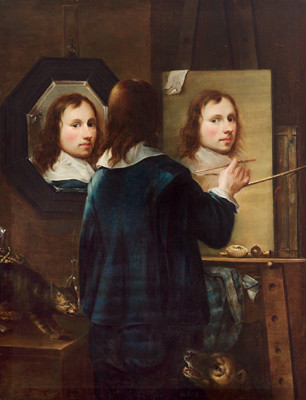
\includegraphics[width=5.0cm]{gumpp.jpeg}
      \caption{Gumpp}
      \centering
    \end{figure}
    
\end{minipage}
\end{tabular}

 \subsubsection{LISP mis en abyme} 
C'est ici un exercice assez classique.
Nous avons fait le choix d'un interprète avec liaison dynamique.
Nous aurons ainsi l'évaluation suivante retournant 13 et non 10.
\begin{Verbatim}
	((evaluate  
	'(let ((a 1))
	  (let ((f (lambda (b) (+ b a)))) 
		 (let ((a 3)) (f 10)))
	)) env)
\end{Verbatim}
En outre, il n'est pas nécessaire d'avoir un mécanisme de point fixe ou d'environnement récursif pour
l'appel d'une fonction récusrsive. C'est l'un des avantages de la liaison dynamique.
\begin{Verbatim}
((evaluate
 '(let ((fact (lambda (n) (if (= n 0) 1 (* n (fact (- n 1)))))))
   (fact 6)))
 env)
\end{Verbatim}


\section{L'auto-interprétation de l'interprète}
En rendant explicite la procédure \verb+eval+ et ses acolytes \verb+evlis, invoke, ...+ dans l'environnement
\verb+env+ , la procédure \verb+evaluate+ pourra être évaluée par elle-même. Le premier argument évalué de la fonction
est le symbole \verb+env+. Ce symbole devra être contenu dans l'environnement \verb+env+, c'est-à-dire dans lui-même\dots

Nous avons \verb+(eval '(eval '+$\pi$ \verb+ env) env)+ $\equiv$ 
 \verb+(evaluate '+$\pi$ \verb+ env)+ 

\subsection{La tour de Babel}

\begin{tikzpicture} 
%environnement

\tikzstyle{estun}=[->,>=latex]
\draw[estun] (-1.5,4.9) to [bend right] (-2, 5.3) to[bend right] (-2.5, 5) ;
\draw (-3, 0) node[above right]{\verb+eval.<proc>+}--(-0.5,0)--(-0.5,5)--(-3,5)
              node[below right]{\verb+env. #env+} --(-3,0) ;
    \node at (-3,2) [right]{\verb+evlis.<proc>+} ;

%the tower
  \draw (-3.5,-1)-- node[above]{$\mathcal{SCHEME}$} (6.5,-1) -- (6.5,-0.5)  -- (-3.5,-0.5) --(-3.5,-1) ;
	\draw (0,0)--node[above]{$\mathcal{I}_0$} (6,0) -- (6,1) node[below right]{\verb+(eval +$'\pi$\verb+ env)+}-- (0,1) -- (0,0) ;
	\draw (0.5,1)--node[above]{$\mathcal{I}_1$}(5.5,1) -- (5.5,2) node[below right]{\verb+(eval '(eval +$'\pi$\verb+ env) env)+}  -- (0.5,2) --(0.5,1) ;
	\draw (1,2)--node[above]{$\mathcal{I}_2$}(5,2) -- (5,3) node[below right]{\verb+(eval '(eval '(eval +$'\pi$\verb+ env) env) env)+} -- (1,3) --(1,2) ;
	\draw (1.5,3)--node[above]{$\mathcal{I}_3$}(4.5,3) -- (4.5,4) node[below right]{\verb+(eval '(eval '(eval '(eval +$'\pi$\verb+ env) env) env) env)+}-- (1.5,4) --(1.5,3) ;
  \draw (2,4)-- node[above]{$\mathcal{I}_4$} (4,4) -- (4,5) node[below right]{\ldots} -- (2,5) --(2,4) ;
  \draw (2,4)-- node[above]{$\mathcal{I}_4$} (4,4) -- (4,5) node[below right]{\ldots} -- (2,5) --(2,4) ;
  \node at (3,5.4) {\vdots} ;
  \node at (3,5.8) {$\mathcal{I}_\infty $} ;

\end{tikzpicture}

\begin{Verbatim}
	((evaluate (quote ((evaluate (quote ((evaluate (quote ((evaluate (quote (
		(lambda (x y) (+ x y)) (fact 5) (fact 6) )))
				   env))) env))) env))) env)
\end{Verbatim}

\subsubsection{L'environnement}
L'environnement doit contenir la valeur du symbole \verb+env+. Il doit faire référence à lui-même.
Seule une liste mutable peut modéliser cette boucle infinie. 
\begin{Verbatim}
> env ; affichage de l'environnement récursif avec DrRacket
#0=((env . #0#)
    (not . #<procedure:...interpreter2.scm:15:17>)
    (= . #<procedure:...interpreter2.scm:16:15>)
    (* . #<procedure:...interpreter2.scm:17:17>)
    (- . #<procedure:...interpreter2.scm:18:17>)
    (+ . #<procedure:...interpreter2.scm:19:17>)
    (atom? . #<procedure:...interpreter2.scm:20:19>)
    (boolean? . #<procedure:...interpreter2.scm:21:22>)
    (number? . #<procedure:...interpreter2.scm:22:21>)
    (cons . #<procedure:...interpreter2.scm:23:18>)
    (car . #<procedure:...interpreter2.scm:24:17>)
    (cdr . #<procedure:...interpreter2.scm:25:17>)
    (pair? . #<procedure:...interpreter2.scm:34:19>)
    (apply . #<procedure:...interpreter2.scm:36:22>)
    (fact . #<procedure:...interpreter2.scm:46:20>)
    (lookup . #<procedure:...interpreter2.scm:53:21>)
    (eprogn . #<procedure:...interpreter2.scm:63:21>)
    (evlis . #<procedure:...interpreter2.scm:74:20>)
    (invoke . #<procedure:...interpreter2.scm:85:14>)
    (extend . #<procedure:...interpreter2.scm:94:18>)
    (mapcar . #<procedure:...interpreter2.scm:105:18>)
    (mapcadr . #<procedure:...interpreter2.scm:113:19>)
    (evallet . #<procedure:...interpreter2.scm:121:6>)
    (evaluate . #<procedure:...interpreter2.scm:128:16>))
\end{Verbatim}

\subsection{Réification et réflexion}
La \textit{réification} est le fait de rendre concrète une chose abstraite.
Dans le cas de notre tour de Babel, réifier un objet du langage d'implémentation le rendra accessible au langage implémenté.
On peut citer l'exemple de la fonction \verb+eval+ rendant accessible dans Scheme le process d'évaluation. 
\verb+(eval '+$\pi$ \verb+) = + $\pi$

L'autre exemple que nous implémenterons est la réification de la continuation courante, mis à disposition
par la fonction \verb+call/cc+. Cette fonction prend en argument une lambda avec un seul paramètre qui récupère la
continuation courante de l'expression en cours d'évaluation.
\begin{Verbatim}
E = (e1 e2 ... (call/cc (lambda (k) ei)) ... en)	
\end{Verbatim}
  Si \verb+ei+ ne fait pas appel à \verb+k+, alors \verb+ei+ est évaluée normalement, ainsi que \verb+E+. 
Dans le cas contraire, \verb+k+ est appelée, liée à la continuation courante. Le résultat de \verb+ei+ est ainsi rendue
à cette continuation capturée \verb+(e1 ... [] ... en)+. Autrement écrit \verb+k = (lambda(v) (e1 ... v ... en))+
\begin{Verbatim}
(+ 5 (call/cc (lambda (k) (* 2 (k 8)))))  = 12
\end{Verbatim} 


L'environnement \verb+global-env+ partagé avec les différents interprètes $\mathcal{I}_i$ de notre tour de babel est aussi considéré
comme un environnement réifié. L'environnement du langage d'implémentation est ici mis à disposition aux langages implémentés.


La \textit{réflection} peut être vue comme l'opération inverse de la réification.
Elle permet la mise à disposition dans le langage d'implémentation un objet du langage implémenté.
Comme exemple, citons la fonction \verb+quote+ qui n'évalue pas son argument et le rend tel quel. \verb+quote+ est
 une primitive du langage Scheme dans le 
sens où il n'est pas possible  de redéfinir cette fonction avec les autre éléments du langage.
Avec l'implémentation de l'interprète $\mathcal{I}_R$ permettant les opérations de réflection et réification,
 cela deviendra possible. 

Pour faire court, la réflection est une opération d'abstraction ; la réification est l'application d'une abstraction.
Ce sont ainsi deux opérations réciproques. 
Voici ce que nous donne pour information la définition du terme \textit{abstraction} recherché dans notre dictionnaire.
\begin{definition}
  L'abstraction désigne le produit de l'opération qui consiste à isoler par la pensée une ou plusieurs qualités d'un objet
  concret pour en former une représentation intellectuelle
    
\end{definition} 

\vspace{0.5cm}

\begin{tabular}{c|c|c} \hline
réification & program vers data &  \verb+((reifier-to-cloture proc) (cdr e) r k)+   \\ \hline
réflection  & data vers program & \verb+(cloture-to-reifier (lambda (e r k) exp))+ \\ \hline
\end{tabular}


\subsubsection{L'interprète par continuation }
La fonction d'évaluation sera enrichie pour prendre trois arguments, le programme $\pi$ à évaluer, l'environnement 
$\rho$ et la continuation $\kappa$ 
\begin{center}
\verb+(eval+ $\pi\ \rho\ \kappa$ \verb+)+ \imp\  \verb+valeur+
\end{center}

Nous reprenons ici le code de l'excellent article \textit{a Simple Reflective Interpreter} \cite{reflective}
La fonction \verb+evaluate+ implémente un interprète Lisp en mode CPS de manière très naturelle.
La valeur ajoutée de l'article est la modélisation des fonctions. Trois types sont disponibles et 
distinguées par un tag dans l'environnement.
\begin{enumerate}
  \item Les fonctions utilisateurs \verb+(cloture (parl) exp env)+
  \item Les fonctions réifiées \verb+(reifier (e r k ) exp )+
  \item Les fonctions primitives \verb+(primitive nom )+
\end{enumerate}
L'application d'une fonction utilisateur se fait de manière classique par une évaluation du corps
de la lambda sur un environnement étendu aux nouvelles liaisons entre paramètres et arguments préalablement évalués.

Une fonction réifiée prend trois paramètres \verb+e+, \verb+r+ et \verb+k+.
\begin{itemize}
  \item  \verb+e+ est lié à la liste des arguments non évalués de l'application.
  \item \verb+r+ est lié à l'environnement de l'interprète évaluant l'application.
  \item \verb+k+ est lié à la continuation de l'interprète évaluant l'application.
\end{itemize}
Ainsi, nous avons un contrôle \textit{complet} de la fonction réifiée : contrôle du corps de la fonction et des arguments
non encore évalués par l'interprète sous-jacent, mais aussi la possibilité d'accéder à l'environnement et à la continuation
courante. En bref, no limit, on peut tout définir\dots

Les fonctions \verb+callcc+ et \verb+quote+ seront très simplement codées de la manière suivante:
\begin{Verbatim}
(define callcc (cloture-to-reifier (lambda (e r k) ((evaluate (car e) r id) k))))
(define quote (cloture-to-reifier (lambda (e r k) (k (car e) ))))
\end{Verbatim}


Dès le niveau 1 de notre tour, c'est-à-dire lorsque la fonction \verb+evaluate+ n'est plus évaluée par Scheme 
mais par elle-même, les formes spéciales \verb+if, quote, begin, define+ sont représentées par des fonctions réifiées.
La fonction d'évaluation peut ainsi être réduite à son strict minimum :
\begin{Verbatim}
(define evaluate
  (lambda (e r k)
    ((if (pair? e)
        (if (equal? (car e) 'lambda)
            eval-abstraction
            eval-application)
        (if (or (or (number? e) (string? e)) (boolean? e))
            eval-constante
            eval-variable))  
     e r k )))
\end{Verbatim}


\begin{minipage}{10.5cm}
  La fonction \verb+openloop+ peut être lancée à volonté et peut créer une succession 
  de  nouveaux étages dans notre tour de babel.
  Comme dans l'épisode biblique du livre de la Genèse\cite{genese}, 
  la faculté d'avoir un langage commun permet la construction
  d'une tour de hauteur potentiellement infinie.
   Nous nous retrouvons nous-même grisés par cette tour \textit{dont la tête touche les cieux}
  (\textgreek{ἡ κεφαλὴ ἔσται ἕως τοῦ οὐρανοῦ}). Nous citons ici la Septante (LXX).
  
  L'enthousiasme de pouvoir
  monter dans les étages doit cependant être tempéré. Le fait d'être à l'étage 
  $n+1$ n'apporte rien par rapport à l'étage $n$. L'application \verb+eval+ est idempotente car 
  $\forall \pi$ \verb+(eval '+$\pi$\verb+)+ $=$ \verb+(eval (eval '+ $\pi$\verb+))+.
  Autrement dit, la valeur \verb+(eval'+$\pi$\verb+)+ est un point fixe de \verb+eval+.
 

  \end{minipage}
  \hfill
  \begin{minipage}{5cm}
    \begin{figure}[H]
      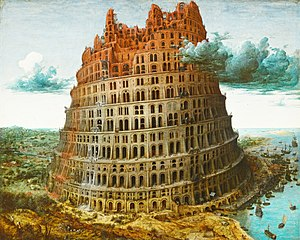
\includegraphics[width=5.0cm]{bruegel.jpg}
      \caption{Bruegel}
      \centering
    \end{figure}
    
\end{minipage}

\vspace{0.5cm}

\textgreek{ΓΕΝΕΣΙΣ     11 \\
  1. Καὶ ἦν πᾶσα ἡ γῆ χεῖλος ἕν, καὶ φωνὴ μία πᾶσιν. \\
   (...) \\ 
  9. διὰ τοῦτο ἐκλήθη τὸ ὄνομα αὐτῆς Σύγχυσις, ὅτι ἐκεῖ συνέχεεν κύριος τὰ χείλη πάσης τῆς γῆς.
}
\textit{\noindent
  Toute la terre avait alors une même parole ; il y avait une seule langue pour tous. \\ 
  À cause de cela, ce lieu fut appelé Babel (confusion), parce que là le Seigneur confondit les langues de toute la terre.
}

\vspace{0.3cm}
En pratique, malheureusement dès le niveau 3 de notre tour, les temps d'évaluation deviennent abominablement longs sur 
notre interprète  maison implémenté en OCAML.
Plusieurs minutes sont requises pour le calcul de la factorielle de cinq au niveau 3 de la tour.
C'est un peux plus rapide avec DrRacket, mais pas tellement. Le poids des sous-couches d'interprétation est lourd.
Dieu ne nous disperse pas ici par la confusion des langages, mais par la limitation de notre puissance de calcul \Laughey .


Voici le code complet de l'interprète au niveau 1. La fonction d'évaluation n'utilise pas ici
les réifications des fonctions \verb+if, quote, begin+.

\begin{footnotesize}
\begin{Verbatim}
(define evaluate
  (lambda (e r k)
    ((if (not (pair? e))
          (if (or (or (number? e) (string? e)) (boolean? e))
              eval-constante
              eval-variable)
          (if (equal? (car e) 'quote)
              eval-quote
              (if (equal? (car e) 'if)
               eval-if
                (if (equal? (car e) 'begin)
               eval-begin
               (if (equal? (car e) 'define)
                   eval-assign
                   (if (equal? (car e) 'lambda)
                       eval-abstraction
                       eval-application))))))
     e r k )))

(define eval-constante
  (lambda (e r k)
    (k e)))

(define eval-quote
  (lambda (e r k)
    (k (cadr e))))

(define eval-variable
  (lambda (e r k)
   (get-pair e r
   (lambda (success-pair)
    (k (cdr success-pair)))
    (lambda ()
    (wrong "symbol not bound " e)))))

(define eval-if
  (lambda (e r k)
    (evaluate (cadr e) r
              (lambda (v)
                (if v
                    (evaluate (caddr e) r k)
                    (evaluate (cadddr e) r k))))))

(define eval-assign
     (lambda (e r k)
       (evaluate (caddr e) r
                 (lambda (v)
                   (get-pair (cadr e) r
                             (lambda (success-pair)
                               (begin
                               (set-cdr! success-pair v)
                               (k (void)) ))
                             (lambda ()
                               (begin
                              (set-cdr! global-env (cons (car global-env)(cdr global-env)))
                              (set-car! global-env (cons (cadr e) v))
                              (k (void)))))))))

(define eval-define
  (lambda (e r k)
      (evaluate (caddr e) r
			(lambda (v) 
			(update! (cadr e) r v))))) 

(define eval-abstraction
  (lambda (e r k)
  (k (make-function (cadr e) (caddr e) r))))
					
(define get-pair
  (lambda (id r success failure)
    (find-pair id r
               success
               (lambda ()
                 (find-pair
                    id global-env success failure) )) ))

(define find-pair
  (lambda (elt alist success failure)
    ( (lambda (assq-result)
        (if assq-result
            (success assq-result)
            (failure)) )
      (assq elt alist) ) ) )

(define make-function
  (lambda (varl corps r)
     (list 'cloture varl corps r)))

(define eval-application
  (lambda (e r k)
       (evaluate (car e) r
              (lambda (proc)
                (if (equal? (car proc) 'reifier)
                    ((reifier-to-cloture proc) (cdr e) r k)
                    (evlis (cdr e) r
                       (lambda (args)
                         (apply-procedure proc args k))))))))

(define evlis
  (lambda (e r k)
    (if (null? e)
        (k '())
        (evaluate (car e) r
                  (lambda (v)
                    (evlis (cdr e) r
                           (lambda (w)
                            (k (cons v w)))))))))

(define eval-begin
  (lambda (e r k)
    (eprogn (cdr e) r k)))

(define eprogn
  (lambda (e r k)
   (if (null? (cdr e))
       (evaluate (car e) r k)
       (evaluate (car e) r (lambda (v)
                             (eprogn (cdr e) r k))))))

(define extend
  (lambda (env variables values)
        (if (or (null? variables) (null? values))
            env
            (cons (cons (car variables) (car values))
                  (extend env (cdr variables) (cdr values))))))
         
(define apply-procedure
  (lambda (proc args k)
    (if (equal? (car proc) 'cloture)
        (eprogn (list (caddr proc))
                (extend (cadddr proc) (cadr proc) args)
                k)
        (k (apply-primitive (cadr proc) args))))) 

(define apply-primitive
  (lambda (name args)
    (if (equal? name 'car)
        (car (car args))
     (if (equal? name 'or)
        (or (car args) (cadr args))
    (if (equal? name 'cdr)
        (cdr (car args))
    (if (equal? name 'cons)
        (cons (car args) (cadr args))
    (if (equal? name 'set-car!)
        (set-car! (car args) (cadr args))
    (if (equal? name 'set-cdr!)
        (set-cdr! (car args) (cadr args))
    (if (equal? name 'memq)
        (memq (car args) (cadr args))
    (if (equal? name 'assq)
        (assq (car args) (cadr args))    
    (if (equal? name '=)
        (= (car args) (cadr args))
    (if (equal? name '+)
        (+ (car args) (cadr args))
    (if (equal? name '-)
        (- (car args) (cadr args))
    (if (equal? name '*)
        (* (car args) (cadr args))
    (if (equal? name 'null?)
        (null? (car args))
    (if (equal? name 'not)
        (not (car args))    
    (if (equal? name 'symbol?)
        (symbol? (car args))
    (if (equal? name 'list)
        args
    (if (equal? name 'pair?)
        (pair? (car args))
    (if (equal? name 'read)
        (if (null? args) (read) (read (car args)))
    (if (equal? name 'eof-object?)
        (eof-object? (car args))
    (if (equal? name 'close-input-port)
        (close-input-port (car args))
    (if (equal? name 'newline)
        (newline)
    (if (equal? name 'equal?)
        (equal? (car args) (cadr args)) 
    (if (equal? name 'write)
        (write (car args))
    (if (equal? name 'display)
        (display (car args))
    (if (equal? name 'load)
        (load (car args)) 
    (if (equal? name 'number?)
        (number? (car args))   
    (if (equal? name 'string?)
        (string? (car args))   
    (if (equal? name 'boolean?)
        (boolean? (car args))   
     "erreur apply primitive"))))))))))))))))))))))))))))))

(define mapper
  (lambda (f l)
    (if (null? l)
        '()
        (cons (f (car l)) (mapper f (cdr l))))))

(define primitive-identifiers
  (lambda ()
    '(placeholder car cdr cons + - * = set-car! set-cdr! memq assq null? equal? newline  
      display read symbol? list pair? not load or number? string? boolean?)))

(define make-primitive
  (lambda (op)
    (list 'primitive op)))

(define reifier-to-cloture
  (lambda (reifier)
    (cons 'cloture (cdr reifier))))

(define cloture-to-reifier
  (lambda (cloture)
    (cons 'reifier (cdr cloture))))

(define make-reifier
  (lambda (formals body r)
    (list 'reifier formals body r)))

(define global-env '())

(define initialize-global-env
  (lambda ()
     (define global-env
      (extend global-env 
          (primitive-identifiers)
          (mapper make-primitive
                  (primitive-identifiers)))))) 

(define openloop
  (lambda (read-prompt write-prompt)
    (begin 
    (display read-prompt)
    (evaluate (read) '()
              (lambda (v)
                (begin
                (display write-prompt)
                (if (equal? v (void))
                  "rien a afficher"
                  (display v))
                (newline)
                (openloop read-prompt write-prompt)))))))

(define babel
  (lambda ()
       (begin
       (set-car! global-env (cons 'global-env global-env ))
       (openloop "i0 " "i0 "))))
\end{Verbatim}
\end{footnotesize}



% La compilation
\chapter{La compilation}
\section{Compilation des $\lambda$-termes en termes applicatifs}
Il existe un formalisme appelé \textit{Logique Combinatoire} qui permet de construire
un calcul sans variables liées. 
C'est surprenant, mais ces variables liées qui sont introduites par abstraction puis éliminées par application
ne sont finalement pas essentielles pour le calcul.

Comment traduire une abstraction en termes applicatifs ? 
Nous allons définir une traduction $M\mapsto  M_@$ , ainsi qu'une traduction en sens inverse
$A\mapsto A_\lambda$.

L'idée est de partir sur les règles de traduction suivantes :
\[
\begin{array}{lcl}
	\lceil \lambda x . x \rceil &=& I \\
	\lceil \lambda x . M \rceil &=& K M \quad (x \notin M) \\
	\lceil \lambda x . M N \rceil &=& S \lceil \lambda x . M \rceil \lceil \lambda x . N \rceil \quad (x \in M,N) \\
\end{array}
\]
où $ \lceil T \rceil$ représente le $\lambda$-terme $T$ sans lambda abstraction. 

Nous serions tentés de vouloir faire directement la traduction en utilisant ces règles.
Il nous faut cependant passer par un opérateur d'abstraction $A \mapsto [x].A$ qui permettra de "supprimer" toutes 
les lambdas en profondeur dans le $\lambda$-terme, puis seulement ensuite, nous pourrons utiliser les trois règles ci-dessous:
\[
\begin{array}{lcl}
	{[x]}  . x   &\equiv & I \\
	{[x]} .  A   &\equiv & K A \quad (x \notin A) \\
	{[x]}  . A B &\equiv & S ([x] . A)([x] . B)  \quad (x \in A,B) \\
\end{array}
\]

Les combinateurs $I, K$ et $S$ sont définis comme ceci:
\[
\begin{array}{ccc}
	I &=& \lambda x . x \\
	K &=& \lambda x y . x \\
	S &=& \lambda x y z . x z (y z) \\
\end{array}	
\]

Et voici la définition de la traduction des $\lambda$-termes en termes applicatifs.
\[
\begin{array}{lcl}
	 (x)_@  &\equiv & x \\
	(PQ)_@  &\equiv & (P)_@ (Q)_@ \\
	(\lambda x.M)_@  &\equiv & [x] .(M)_@   \\
\end{array}
\]

Dans la définition de notre type applicatif \verb+ski+, nous incluons aussi notre opérateur $[x].A$ 
avec le constructeur \verb+Op+.

\begin{Verbatim}
type ski = 
| Varia of string
| I
| K
| S
| Appl of ski*ski 
| Op of string * ski ;;

exception SkiExec

let rec lambda_ski = function
| Lam(x, t) -> lambda_ski_op (Op(x, lambda_ski t))
| Var(x) -> Varia(x)
| App(m,n) -> Appl(lambda_ski m, lambda_ski n) 
and lambda_ski_op = function
| Op(x,Varia y) when x=y -> I 
| Op(x, t) when not (mem x (var t)) -> Appl(K, t) 
| Op(x, Appl(m, n))  when (mem x (var m)) || (mem x (var n)) 
	  -> Appl(Appl(S, (lambda_ski_op (Op(x,m)))), (lambda_ski_op (Op(x,n)))) 
| _ -> raise SkiErreur
\end{Verbatim}
A titre d'exemple, traduisons notre combinateur $y$ en termes applicatifs:
\begin{Verbatim}
utop # print_ski (lambda_ski y) ;;
((S((S((S(KS))((S(KK))I)))(K((SI)I))))((S((S(KS))((S(KK))I)))(K((SI)I))))
\end{Verbatim}
Une fois le code compilé, son exécution sera réalisée avec les règles de réécriture :
\[
\begin{array}{ccc}
	Ix &\longrightarrow & x \\
	Kxy &\longrightarrow & x \\
	Sxyz &\longrightarrow & x z (y z)	\\
\end{array}	
\]
Voici une première version de l'exécution de ces règles de réécriture. Ce code un est peu bourrin car on appelle
la fonction tant que le terme n'est pas réduit.
\begin{Verbatim}
let rec exec_aux = function
| Appl(I, x) -> exec_aux x
| Appl(Appl(K, x), y) -> exec_aux x
| Appl(Appl(Appl(S,x),y),z) -> Appl(Appl(exec_aux x, exec_aux z), Appl(exec_aux y,exec_aux z))
| Appl(x,y) -> Appl(exec_aux x, exec_aux y)
| Varia x -> Varia x
| I -> I
| K -> K
| S -> S
| _ -> raise SkiErreur 
and  exec t =
let r = exec_aux t in
	if r=t then r else exec_aux r 
\end{Verbatim}

Voici une version plus élégante qui retourne la forme réduite.
\begin{Verbatim}
let rec ski_norm m =
match m with
| S | K | I -> m
| Varia x -> m
| Appl (m0, m1) ->
match ski_norm m0 with
| I -> ski_norm m1
| Appl (K, m') -> m'
| Appl (Appl (S, m3), m2) -> ski_norm (Appl (Appl (m3, m1), Appl (m2, m1)))
| autre -> Appl (autre, ski_norm m1);;
\end{Verbatim}

La traduction en sens inverse $A \mapsto A_\lambda $ se fait naturellement par la fonction ML ci-dessous:
\begin{Verbatim}
let rec ski_lambda = function
| I -> Lam("x", Var "x")
| K -> Lam("x", Lam("y", Var "x"))
| S -> Lam("x", Lam("y", Lam("z", App(App(Var "x", Var "z"), App(Var "y", Var "z")))))
| Varia(x) -> Var(x)
| Appl(m,n) -> App(ski_lambda m,ski_lambda n)
| _ -> raise SkiErreur
\end{Verbatim}

Utilisons l'exemple de la factorielle, exemple complexe car il comporte les représentations en $\lambda$-termes
du combinateur $Y$, de la condition \textit{if-then-else}, des entiers \textit{Church} ainsi que les opérations
\textit{plus, moins, mult}.\footnote{Ce résultat est obtenu après quelques minutes...}
\begin{Verbatim}
print_terme (betaNormal (ski_lambda (exec (lambda_ski (App(fact, trois)))))) ;;
λz.λz0.z (z (z (z (z (z z0) ) ) ) ) - : unit = ()	
\end{Verbatim}

Nous avons les deux propriétés suivantes que nous ne démontrerons pas.
\begin{enumerate}
	\item Si $A \trans B$, alors $A_\lambda \trans B_\lambda$ \\
	\item $(M_@)_\lambda \trans M $ \\
\end{enumerate}


Cependant, nous aurons parfois $M \longrightarrow_\beta N$ sans que $M_@ \longrightarrow_@ N_@$

Par exemple $SK \trans 0$ mais $SK$ est irréductible pour $\longrightarrow_@$
\begin{Verbatim}
utop # betaNormalPrint sk ;;
[1] -> λx.λy.λz.x z (y z)  λx.λy.x
[2] -> λy.λz.λx.λy.x z (y z) 
[3] -> λy.λz.λy.z (y z) 
[4] -> λy.λz.z
- : unit -> unit = <fun>	

utop # exec (Appl(S,K)) ;;
- : ski = Appl (S, K)
\end{Verbatim}

D'autre part, on n'a pas nécessairement $(A_\lambda)_@ =_@ A$.

Par exemple $(K_\lambda)_@ \equiv S(KK)I$  ne se réduit pas en $K$.
\begin{Verbatim}
utop # exec (lambda_ski k) ;;
- : ski = Appl (Appl (S, Appl (K, K)), I)

betaNormalPrint (App(App(s, App (k, k)), i)) ;;
[1] -> λx.λy.λz.x z (y z)  (λx.λy.x λx.λy.x)  λx.x
[2] -> λy.λz.λx.λy.x λx.λy.x z (y z)  λx.x
[3] -> λz.λx.λy.x λx.λy.x z (λx.x z) 
[4] -> λz.λy.λx.λy.x z (λx.x z) 
[5] -> λz.λx.λy.x (λx.x z) 
[6] -> λz.λy.λx.x z
[7] -> λz.λy.z
- : unit -> unit = <fun>
\end{Verbatim}
On peut constater que $(SKK)x \trans x $, donc le terme $SKK$ joue le même rôle
que la constante $I$. 
\begin{Verbatim}
let skk = Appl(Appl(S,K),K) ;;
exec (Appl(skk, Varia "x")) ;;
- : ski = Varia "x"
\end{Verbatim}
ou plus directement en \sc{Ocaml}:
\begin{Verbatim}
utop # 
let k x y = x
and s x y z = (x z (y z)) 
  in (s k k) "toto ";;
- : string = "toto "
\end{Verbatim}
La base combinatoire $\{S,K\}$ suffit donc au $\lambda$-calcul. 
Une base à un seul élément existerait même\dots

\subsubsection{La correspondance de Curry-Howard}
Dans un $\lambda$-calcul typé, les types des combinateurs $K$ et $S$ correspondent aux deux axiomes
des systèmes hilbertiens :
$$ S : (\phi \Rightarrow (\chi \Rightarrow \psi)) \Rightarrow ((\phi \Rightarrow \chi) \Rightarrow(\phi \Rightarrow \psi)) 
$$
$$   K : \phi \Rightarrow (\psi \Rightarrow \phi)
$$
L'inférence de type OCAML nous donne en effet 
\verb+k : 'a -> 'b -> 'a+ et  \\ 
\verb+ s : ('a -> 'b -> 'c) -> ('a -> 'b) -> 'a -> 'c+
\begin{center}
\begin{figure}[H]
	\begin{tabular}{|c|c|} \hline
		\textit{logique combinatoire} & \textit{système hilbertien} \\ \hline
		type & formule \\
		application (\textbf{App}) & modus ponens \\
		combinateurs $S$ et $K$ & noms des axiomes $S$ et $K$ \\
		type des combinateurs $S$ et $K$ & axiomes $S$ et $K$ \\
		variable & nom d'une hypothèse \\
		type d'une variable & hypothèse \\ \hline
	\end{tabular}	
\end{figure}
\end{center}

L'unique règle d'inférence, la règle du modus ponens, est ainsi modélisée par l'application
$$ (App) : \frac{\phi \Rightarrow \psi \ \ \phi}{\psi} $$

Dans le système hilbertien, il n'y a pas de règle d'introduction 
$(I_\Rightarrow) : \frac{[\phi]\ \ \chi}{\phi \Rightarrow \chi}$ qui équivalait à une abstraction 
$\lambda x^\phi.y^\psi $

Le modus ponens et les axiomes permettent de simuler $(I_\Rightarrow )$ de la même façon que 
l'abstraction du $\lambda$-calcul est simulée à l'aide des constantes $S$ et $K$ en logique combinatoire.


\section{Compilation basique vers une machine à pile}
Nous utilisons l'implémentation ci-dessous pour la représentation des piles sous
formes de listes mutables.
\begin{Verbatim}
type 'a pile = 'a list ref ;;
let empiler x p = p := x :: !p ;;

exception Vide ;;

let depiler p =  
	match !p with
  | [] -> raise Vide
  |x::t -> p:=t ; x ;;

let sommet p =
	match !p with
	| [] -> raise Vide
	| x::t -> x  ;;
\end{Verbatim}

La machine à pile exécutera les instructions suivantes:\\
\verb+["EMPILER"; "nombre"],["ADD"], ["SUB"], ["MUL"], ["STOP"]+

La lecture d'une instruction est réalisée par la fonction \texttt{fetch}. Cette
fonction parcourt de manière linéaire le code représenté par un \textit{array}.
Chaque \texttt{fetch} incrémente la variable \verb+pc+ qui représente le
\textit{program counter}.

\begin{Verbatim}
exception Erreur ;;
	
let executer code =
	let pc = ref 0 in
	let pile = ref [] in
	let fetch code  =
	begin
		pc := !pc + 1 ; 
		Array.get code (!pc - 1) 
	end 
	in
	let rec exec () =
		let instr = fetch code in
		match instr with
		| ["EMPILER"; n] -> ( empiler (int_of_string n) pile ; exec () )
		| ["ADD"] -> let v2 = depiler pile in let v1 = depiler pile in 
		            ( empiler (v1 + v2) pile ; exec () )
		| ["SUB"] -> let v2 = depiler pile in let v1 = depiler pile in
		            ( empiler (v1 - v2) pile ; exec () )
		| ["MUL"] -> let v2 = depiler pile in let v1 = depiler pile in
		            ( empiler (v1 * v2) pile ; exec () )
		| ["STOP"] -> print_int (sommet pile)
		| _ -> raise Erreur
	in exec ()
\end{Verbatim}

Voici l'exécution de la machine à pile:
\begin{Verbatim}
let code = [| ["EMPILER"; "10"] ;["EMPILER"; "15"] ; ["ADD"] ;
						  ["EMPILER"; "4"] ; ["MUL"] ; ["STOP"] |] ;;
						  
# executer code ;;
# 100- : unit = ()
\end{Verbatim}

\subsection{Certification de la compilation avec le langage \textsc{Coq}}
\textit{Quod erat demonstrandum.}
\begin{center}
\begin{tikzpicture}
 \node at(0,6) {$e$} ;
 \node at(6,6) {$c$} ;
 \node at(6,0) {$v_2$} ;
 \node at(0,0) {$v_1$} ;
\draw[dashed] (0.3,0) -- node[below]{$v_1=v_2$} node[above]{$\forall e, eval(e)= exe(compile\ e)$}(5.7,0)  ;
\draw[-latex] (6,5.7) -- node[rotate=-90, below]{sémantique de la machine } (6,0.3) ;
\draw[-latex] (0.3,6) -- node[below]{sémantique du compilateur } (5.7,6) ;
\draw[-latex] (0,5.7) -- node[rotate=-90, above]{sémantique du langage } (0,0.3);
\end{tikzpicture}
\end{center}

\vspace{0.5cm}
%%%%%%%%%%%%%%%%%%%%%%%%%%%%%%%%%%%%%%%%%%%%%%%%%%%%%%%%%%%%%%%%%
%% This file has been automatically generated with the command
%% coqdoc --latex premier.v 
%%%%%%%%%%%%%%%%%%%%%%%%%%%%%%%%%%%%%%%%%%%%%%%%%%%%%%%%%%%%%%%%%


\begin{coqdoccode}
\coqdocnoindent
\coqdockw{Require} \coqdockw{Import} \coqdocvar{Arith}.\coqdoceol
\coqdocnoindent
\coqdockw{Require} \coqdockw{Import} \coqdocvar{ZArith}.\coqdoceol
\coqdocnoindent
\coqdockw{Require} \coqdockw{Import} \coqdocvar{Bool}.\coqdoceol
\coqdocnoindent
\coqdockw{Require} \coqdockw{Import} \coqdocvar{List}.\coqdoceol
\coqdocemptyline
\coqdocnoindent
\coqdockw{Inductive} \coqdocvar{exp} : \coqdockw{Set} :=\coqdoceol
\coqdocindent{1.00em}
\ensuremath{|} \coqdocvar{Const} : \coqdocvar{nat} \ensuremath{\rightarrow} \coqdocvar{exp}\coqdoceol
\coqdocindent{1.00em}
\ensuremath{|} \coqdocvar{Fois} : \coqdocvar{exp} \ensuremath{\rightarrow} \coqdocvar{exp} \ensuremath{\rightarrow} \coqdocvar{exp}\coqdoceol
\coqdocindent{1.00em}
\ensuremath{|} \coqdocvar{Plus} : \coqdocvar{exp} \ensuremath{\rightarrow} \coqdocvar{exp} \ensuremath{\rightarrow} \coqdocvar{exp}.\coqdoceol
\coqdocemptyline
\coqdocnoindent
\coqdockw{Fixpoint} \coqdocvar{expEval} (\coqdocvar{e}:\coqdocvar{exp}) : \coqdocvar{nat} :=\coqdoceol
\coqdocindent{1.00em}
\coqdockw{match} \coqdocvar{e} \coqdockw{with}\coqdoceol
\coqdocindent{1.00em}
\ensuremath{|} \coqdocvar{Const} \coqdocvar{n} \ensuremath{\Rightarrow} \coqdocvar{n}\coqdoceol
\coqdocindent{1.00em}
\ensuremath{|} \coqdocvar{Fois} \coqdocvar{e1} \coqdocvar{e2} \ensuremath{\Rightarrow} \coqdocvar{mult}  (\coqdocvar{expEval} \coqdocvar{e1}) (\coqdocvar{expEval} \coqdocvar{e2})\coqdoceol
\coqdocindent{1.00em}
\ensuremath{|} \coqdocvar{Plus} \coqdocvar{e1} \coqdocvar{e2} \ensuremath{\Rightarrow} \coqdocvar{plus} (\coqdocvar{expEval} \coqdocvar{e1}) (\coqdocvar{expEval} \coqdocvar{e2})\coqdoceol
\coqdocindent{1.00em}
\coqdockw{end}.\coqdoceol
\coqdocemptyline
\coqdocnoindent
\coqdockw{Inductive} \coqdocvar{instr} : \coqdockw{Set} :=\coqdoceol
\coqdocindent{0.50em}
\ensuremath{|} \coqdocvar{EMPILER} : \coqdocvar{nat} \ensuremath{\rightarrow} \coqdocvar{instr}\coqdoceol
\coqdocindent{0.50em}
\ensuremath{|} \coqdocvar{ADD} :  \coqdocvar{instr}\coqdoceol
\coqdocindent{0.50em}
\ensuremath{|} \coqdocvar{MUL} : \coqdocvar{instr}\coqdoceol
\coqdocnoindent
.\coqdoceol
\coqdocemptyline
\coqdocnoindent
\coqdockw{Definition} \coqdocvar{programme} := \coqdocvar{list} \coqdocvar{instr}.\coqdoceol
\coqdocnoindent
\coqdockw{Definition} \coqdocvar{pile} := \coqdocvar{list} \coqdocvar{nat}.\coqdoceol
\coqdocemptyline
\coqdocnoindent
\coqdockw{Definition} \coqdocvar{instrExec} (\coqdocvar{i}:\coqdocvar{instr}) (\coqdocvar{s}: \coqdocvar{pile}) : \coqdocvar{option} \coqdocvar{pile}:=\coqdoceol
\coqdocindent{1.00em}
\coqdockw{match} \coqdocvar{i} \coqdockw{with}\coqdoceol
\coqdocindent{1.00em}
\ensuremath{|} \coqdocvar{EMPILER} \coqdocvar{n} \ensuremath{\Rightarrow} \coqdocvar{Some} (\coqdocvar{n} :: \coqdocvar{s})\coqdoceol
\coqdocindent{1.00em}
\ensuremath{|} \coqdocvar{ADD} \ensuremath{\Rightarrow} \coqdoceol
\coqdocindent{2.50em}
\coqdockw{match} \coqdocvar{s} \coqdockw{with}\coqdoceol
\coqdocindent{2.50em}
\ensuremath{|} \coqdocvar{arg1} :: \coqdocvar{arg2} :: \coqdocvar{s'} \ensuremath{\Rightarrow} \coqdocvar{Some} (\coqdocvar{expEval} (\coqdocvar{Plus} (\coqdocvar{Const}(\coqdocvar{arg1})) (\coqdocvar{Const}(\coqdocvar{arg2}))) :: \coqdocvar{s'})\coqdoceol
\coqdocindent{2.50em}
\ensuremath{|} \coqdocvar{\_} \ensuremath{\Rightarrow} \coqdocvar{None}\coqdoceol
\coqdocindent{2.50em}
\coqdockw{end}\coqdoceol
\coqdocindent{1.00em}
\ensuremath{|} \coqdocvar{MUL} \ensuremath{\Rightarrow}\coqdoceol
\coqdocindent{2.50em}
\coqdockw{match} \coqdocvar{s} \coqdockw{with}\coqdoceol
\coqdocindent{2.50em}
\ensuremath{|} \coqdocvar{arg1} :: \coqdocvar{arg2} :: \coqdocvar{s'} \ensuremath{\Rightarrow} \coqdocvar{Some} (\coqdocvar{expEval} (\coqdocvar{Fois} (\coqdocvar{Const}(\coqdocvar{arg1})) (\coqdocvar{Const}(\coqdocvar{arg2}))) ::\coqdocvar{s'})\coqdoceol
\coqdocindent{2.50em}
\ensuremath{|} \coqdocvar{\_} \ensuremath{\Rightarrow} \coqdocvar{None}\coqdoceol
\coqdocindent{2.50em}
\coqdockw{end}\coqdoceol
\coqdocindent{1.00em}
\coqdockw{end}.\coqdoceol
\coqdocemptyline
\coqdocnoindent
\coqdockw{Fixpoint} \coqdocvar{progExec} (\coqdocvar{p}:\coqdocvar{programme})  (\coqdocvar{s}:\coqdocvar{pile}) : \coqdocvar{option} \coqdocvar{pile} :=\coqdoceol
\coqdocindent{1.00em}
\coqdockw{match} \coqdocvar{p} \coqdockw{with} \coqdoceol
\coqdocindent{1.00em}
\ensuremath{|} \coqdocvar{nil} \ensuremath{\Rightarrow} \coqdocvar{Some} \coqdocvar{s}\coqdoceol
\coqdocindent{1.00em}
\ensuremath{|} \coqdocvar{i} :: \coqdocvar{p'} \ensuremath{\Rightarrow} \coqdoceol
\coqdocindent{3.00em}
\coqdockw{match} \coqdocvar{instrExec} \coqdocvar{i} \coqdocvar{s} \coqdockw{with}\coqdoceol
\coqdocindent{3.00em}
\ensuremath{|} \coqdocvar{None} \ensuremath{\Rightarrow} \coqdocvar{None}\coqdoceol
\coqdocindent{3.00em}
\ensuremath{|} \coqdocvar{Some} \coqdocvar{s'} \ensuremath{\Rightarrow} \coqdocvar{progExec} \coqdocvar{p'} \coqdocvar{s'} \coqdoceol
\coqdocindent{3.00em}
\coqdockw{end}\coqdoceol
\coqdocindent{1.00em}
\coqdockw{end}.\coqdoceol
\coqdocemptyline
\coqdocnoindent
\coqdockw{Fixpoint} \coqdocvar{compile} (\coqdocvar{e}:\coqdocvar{exp}) : \coqdocvar{programme} :=\coqdoceol
\coqdocindent{1.00em}
\coqdockw{match} \coqdocvar{e} \coqdockw{with} \coqdoceol
\coqdocindent{1.00em}
\ensuremath{|} \coqdocvar{Const} \coqdocvar{n} \ensuremath{\Rightarrow} \coqdocvar{EMPILER} \coqdocvar{n} :: \coqdocvar{nil}\coqdoceol
\coqdocindent{1.00em}
\ensuremath{|} \coqdocvar{Plus} \coqdocvar{e1} \coqdocvar{e2} \ensuremath{\Rightarrow} \coqdocvar{compile} \coqdocvar{e2} ++ \coqdocvar{compile} \coqdocvar{e1} ++ \coqdocvar{ADD} :: \coqdocvar{nil}\coqdoceol
\coqdocindent{1.00em}
\ensuremath{|} \coqdocvar{Fois} \coqdocvar{e1} \coqdocvar{e2} \ensuremath{\Rightarrow} \coqdocvar{compile} \coqdocvar{e2} ++ \coqdocvar{compile} \coqdocvar{e1} ++ \coqdocvar{MUL} :: \coqdocvar{nil}\coqdoceol
\coqdocindent{1.00em}
\coqdockw{end} .\coqdoceol
\coqdocemptyline
\coqdocnoindent
\coqdockw{Eval} \coqdoctac{compute} \coqdoctac{in} (\coqdocvar{compile} (\coqdocvar{Const} 1999)) .\coqdoceol
\coqdocnoindent
\coqdockw{Eval} \coqdoctac{compute} \coqdoctac{in} (\coqdocvar{compile} (\coqdocvar{Fois} (\coqdocvar{Plus} (\coqdocvar{Const} 1999) (\coqdocvar{Const} 1)) (\coqdocvar{Const} 5))) .\coqdoceol
\coqdocnoindent
\coqdockw{Eval} \coqdoctac{compute} \coqdoctac{in} ( \coqdocvar{progExec} (\coqdocvar{compile} (\coqdocvar{Fois} (\coqdocvar{Plus} (\coqdocvar{Const} 1999) (\coqdocvar{Const} 1)) (\coqdocvar{Const} 5))) \coqdocvar{nil}) .\coqdoceol
\coqdocemptyline
\coqdocnoindent
\coqdockw{Lemma} \coqdocvar{compile\_correct\_lemme}: \coqdockw{\ensuremath{\forall}} (\coqdocvar{e}:\coqdocvar{exp}) (\coqdocvar{p}: \coqdocvar{programme}) (\coqdocvar{s}: \coqdocvar{pile}),\coqdoceol
\coqdocindent{14.00em}
\coqdocvar{progExec} (\coqdocvar{compile} \coqdocvar{e}++\coqdocvar{p}) \coqdocvar{s} = \coqdocvar{progExec} \coqdocvar{p} (\coqdocvar{expEval} \coqdocvar{e}::\coqdocvar{s})\coqdoceol
\coqdocindent{0.50em}
.\coqdoceol
\coqdocindent{0.50em}
\coqdoctac{induction} \coqdocvar{e}.\coqdoceol
\coqdocindent{0.50em}
\coqdoctac{intros}.\coqdoceol
\coqdocindent{0.50em}
\coqdoctac{unfold} \coqdocvar{compile}.\coqdoceol
\coqdocindent{0.50em}
\coqdoctac{unfold} \coqdocvar{expEval}.\coqdoceol
\coqdocindent{0.50em}
\coqdoctac{unfold} \coqdocvar{progExec} \coqdoctac{at} 1.\coqdoceol
\coqdocindent{0.50em}
\coqdoctac{simpl}.\coqdoceol
\coqdocindent{0.50em}
\coqdoctac{fold} \coqdocvar{progExec}.\coqdoceol
\coqdocindent{0.50em}
\coqdoctac{reflexivity}.\coqdoceol
\coqdocemptyline
\coqdocindent{0.50em}
\coqdoctac{intros}.\coqdoceol
\coqdocindent{0.50em}
\coqdoctac{unfold} \coqdocvar{compile}. \coqdoctac{fold} \coqdocvar{compile}.\coqdoceol
\coqdocindent{0.50em}
\coqdoctac{unfold} \coqdocvar{expEval}. \coqdoctac{fold} \coqdocvar{expEval}.\coqdoceol
\coqdocindent{0.50em}
\coqdoctac{rewrite} \coqdocvar{app\_assoc\_reverse}.\coqdoceol
\coqdocindent{0.50em}
\coqdoctac{rewrite} \coqdocvar{IHe2}. \coqdoctac{rewrite} \coqdocvar{app\_assoc\_reverse}.\coqdoceol
\coqdocindent{0.50em}
\coqdoctac{rewrite} \coqdocvar{IHe1}.\coqdoceol
\coqdocindent{0.50em}
\coqdoctac{unfold} \coqdocvar{progExec} \coqdoctac{at} 1. \coqdoctac{simpl}. \coqdoctac{fold} \coqdocvar{progExec}. \coqdoctac{reflexivity}.\coqdoceol
\coqdocemptyline
\coqdocindent{0.50em}
\coqdoctac{intros}.\coqdoceol
\coqdocindent{0.50em}
\coqdoctac{unfold} \coqdocvar{compile}. \coqdoctac{fold} \coqdocvar{compile}.\coqdoceol
\coqdocindent{0.50em}
\coqdoctac{rewrite} \coqdocvar{app\_assoc\_reverse}. \coqdoctac{rewrite} \coqdocvar{IHe2}.\coqdoceol
\coqdocindent{0.50em}
\coqdoctac{rewrite} \coqdocvar{app\_assoc\_reverse}.\coqdoceol
\coqdocindent{0.50em}
\coqdoctac{unfold} \coqdocvar{progExec} \coqdoctac{at} 1. \coqdoctac{simpl}. \coqdoctac{fold} \coqdocvar{progExec}.\coqdoceol
\coqdocindent{0.50em}
\coqdoctac{rewrite} \coqdocvar{IHe1}.\coqdoceol
\coqdocindent{0.50em}
\coqdoctac{unfold} \coqdocvar{progExec} \coqdoctac{at} 1. \coqdoctac{simpl}. \coqdoctac{fold} \coqdocvar{progExec}. \coqdoctac{reflexivity}.\coqdoceol
\coqdocemptyline
\coqdocindent{0.50em}
\coqdockw{Qed}.\coqdoceol
\coqdocemptyline
\coqdocnoindent
\coqdockw{Theorem} \coqdocvar{compile\_correct}: \coqdockw{\ensuremath{\forall}} \coqdocvar{e} : \coqdocvar{exp}, \coqdocvar{Some} ((\coqdocvar{expEval} \coqdocvar{e}) :: \coqdocvar{nil}) = (\coqdocvar{progExec} (\coqdocvar{compile} \coqdocvar{e}) \coqdocvar{nil}).\coqdoceol
\coqdocnoindent
\coqdoctac{intros}.\coqdoceol
\coqdocnoindent
\coqdoctac{rewrite} (\coqdocvar{app\_nil\_end} (\coqdocvar{compile} \coqdocvar{e})).\coqdoceol
\coqdocnoindent
\coqdoctac{rewrite} \coqdocvar{compile\_correct\_lemme}.\coqdoceol
\coqdocnoindent
\coqdoctac{reflexivity}.\coqdoceol
\coqdocnoindent
\coqdockw{Qed}.\coqdoceol
\coqdocemptyline
\coqdocnoindent
\coqdockw{Print} \coqdocvar{compile\_correct}.\coqdoceol
\end{coqdoccode}


\section{Compilation du \textsc{Lisp} vers une machine abstraite}
\subsubsection{La machine SECD}
La machine SECD inventée par Landin est une machine abstraite utilisant quatre composants:
\begin{itemize}
  \item S, la pile ou \textit{stack} permettant de stocker les résultats intermédiaires puis le résultat final
  \item E, l'environnement d'éxecution
  \item C, le code
  \item D, le dump permettant de stocker les valeurs courantes S,E,C le temps d'un calcul local d'une fonction
\end{itemize}
Nous devons implémenter deux fonctions.

La fonction de compilation \verb+compile+ qui prend en argument une expression LISP, 
un environnement de compilation et l'accumulateur du code compilé.
Nous ferons travailler la fonction \verb+compile+ sur la syntaxe abstraite pour plus de facilité.


La fonction d'éxecution  \verb+exe s e c d+  prend en arguments les 
quatre composantes de la machine abstraite.

\subsubsection{La compilation $C: exp$\ \imp\ \texttt{code}}
\noindent
  \texttt{c} \imp\ \texttt{CONST}$(c)$ \\
  \texttt{n} \imp\ \texttt{ACCESS}$(n)$ \\
  \texttt{(+ a1 a2)} \imp\ $C(a_1); C(a_2);$ \texttt{ADD} \\
  \texttt{(- a1 a2)} \imp\ $C(a_1); C(a_2);$ \texttt{SUB} \\
  \texttt{(= a1 a2)} \imp\ $C(a_1); C(a_2);$ \texttt{CMP} \\
  \texttt{((lambda (v1...vn) body) e1...en)} 
    \imp\ \texttt{NIL;} $C(v_1)$\texttt{;ARG;}$\dots C(v_n)$\texttt{;ARG;CLOSURE}$(C(body)$\texttt{;RTS}$)$\texttt{;JSR} \\
  

\subsubsection{La table de transition de la machine SECD}
\begin{footnotesize}
\[
\begin{array}{|c|c|c|c || c|c|c|c|}
  \hline
  \multicolumn{4}{|c||}{\textbf{état avant}} & \multicolumn{4}{c|}{\textbf{état après}} \\
  \hline \hline
  S & E & C & D & S & E & C & D \\
  \hline
  
  s         & e & \texttt{CONST}(cst); c & d                & cst.s         & e & c &  d \\
  n_2.n_1.s & e & \texttt{ADD}; c        & d                & (n_1 + n_2).s & e & c &  d \\
  n_2.n_1.s & e & \texttt{SUB}; c        & d                & (n_1 - n_2).s & e & c &  d \\
  n_2.n_1.s & e & \texttt{CMP}; c        & d                & (n_1 = n_2).s & e & c &  d \\
        s   & e & \mathtt{ACCESS}(n);c   & d                & e(n).s        & e & c &  d \\ 
  \hline \hline
  \multicolumn{8}{|c|}{\textrm{construction d'une liste d'arguments}} \\
  \hline
  s         & e & \mathtt{NIL}; c        & d                & [\ ]   & e & c &  d \\
  v_1.v_2.s & e & \mathtt{ARG}; c        & d                & v_1 @ v_2 . s & e & c &  d \\
  \hline \hline
  \multicolumn{8}{|c|}{\textrm{la conditionnelle}} \\
  \hline
  v.s       & e & \mathtt{BRANCH}(c_1, c_2);c & d             & s             & e & c_1;c & d \\
  v.s       & e & \mathtt{BRANCH}(c_1, c_2);c & d             & s             & e & c_2;c & d \\
  \hline \hline
  \multicolumn{8}{|c|}{\textrm{le traitement d'une clôture}} \\
  \hline
  s         & e &  \mathtt{CLOSURE}(f);c      & d             & \mathtt{CLOS}(f,e) & e & c & d \\
  \hline \hline 
  \multicolumn{8}{|c|}{\textrm{application d'une lambda avec les instructions }\texttt{JSR,RTS}} \\
  \hline 
  \mathtt{CLOS}(f,e_0).largs.s & e & \mathtt{JSR};c & d       & [\ ] & largs::e_0 & f & \mathtt{ENVEXE}(s,e,c).d \\
  v.s & e & \mathtt{RTS};c & \mathtt{ENVEXE}(s_1, e_1, c_1).d & v.s_1 & e_1 & c_1 & d \\     
  \hline
\end{array}
\]

\end{footnotesize}

\subsubsection{L'implémentation en \textsc{Ocaml}}

\begin{footnotesize}
\begin{Verbatim}
let rec compile envc exp codesuivant  =
  match exp with
  | Atom (Entier n) -> CONST n :: codesuivant
  | Var s -> ACCESS (adresse s envc) :: codesuivant
  | Call (f, args) -> compile_call envc f args codesuivant
  | Let (decl,expl) -> compile_let envc decl expl codesuivant 
  | If (cond, exp1, exp2) -> compile_if envc cond exp1 exp2 codesuivant
  | Lambda (parl, bodyl) -> compile_lambda envc parl bodyl codesuivant
  | _ -> raise (Erreur "compile")

and compile_lambda envc parl bodyl codesuivant =
  (CLOSURE ((compile (parl::envc) (hd bodyl)  [RTS])) ) :: codesuivant 

and compile_if envc cond exp1 exp2 codesuivant =
   let code_si = compile envc exp1 codesuivant
   and code_sinon = compile envc exp2 codesuivant
in compile envc cond ( BRANCH(code_si,  code_sinon) :: codesuivant ) 

and compile_call envc f args codesuivant  =
match f with 
 | Var "+" -> compile_app  envc args  (ADD :: codesuivant)
 | Var  "-"  -> compile_app  envc args  (SUB :: codesuivant)
 | Var  "="  -> compile_app  envc args  (CMP :: codesuivant)
 | _ -> compile_larg envc args (compile envc f (JSR :: codesuivant))
 
and
compile_app envc args codesuivant =
  if args = [] then codesuivant
  else  compile envc (hd args) (compile_app envc (tl args) codesuivant) 
and compile_let envc decl expl codesuivant =
  let lvar = map fst decl
  in let lexp = map snd decl
  in compile envc (Call(Lambda(lvar, expl),lexp)) codesuivant 
and compile_larg envc lexp codesuivant =
  let rec aux lexp codesuivant =
    match lexp with
    | [] -> codesuivant
    | a::b -> aux b (compile envc a (ARG::codesuivant))
  in NIL::(aux lexp codesuivant)
    
let rec exe s e c d =
  if (List.length c) = 0 then hd s
  else
    match (hd c) with
  | ADD ->  let Entier(n2) = hd (hd s) and Entier(n1) = hd (hd (tl s)) in
              exe ([Entier(n1+n2)]:: (tl (tl s))) e (tl c) d  
  | SUB ->  let Entier(n2) = hd (hd s) and Entier(n1) = hd (hd (tl s)) in
              exe ([Entier(n1-n2)]:: (tl (tl s))) e (tl c) d  
  | CMP ->  let Entier(n2) = hd (hd s) and Entier(n1) = hd (hd (tl s)) in 
                exe ([Booleen(n1=n2)]:: (tl (tl s))) e (tl c) d   
  | CONST n ->  exe ([Entier n]::s)  e (tl c) d
  | NIL ->  exe ([]::s) e (tl c) d 
  | ARG ->    let v1 = hd s
              in let v2 = hd (tl s)
                in  exe ((v1 @ v2)::(tl (tl s))) e (tl c) d
  | ACCESS sy ->  exe ([lire_env sy e]::s) e (List.tl c) d
  | BRANCH(code_si, code_sinon) ->
          let v = hd (hd s) in 
                if (v = Booleen(true)) then exe (tl s) e (code_si @ (tl c)) d 
                else exe (tl s) e ( code_sinon @ (tl c)) d 
  | CLOSURE(fonc) ->  exe ([CLOS(fonc,e)]::s) e (tl c) d
  | JSR -> let CLOS(corps, e0) = hd (hd s) in
            let larg = hd (tl s) in 
              exe [] (larg::e) corps ((ENVEXE(tl (tl s), e, (tl c)))::d) 
  | RTS -> let ENVEXE(s1, e1, c1) = hd d 
            and v = hd s in
            exe (v::s1) e1 c1 (tl d)
\end{Verbatim}
\end{footnotesize}

% La résolution
\chapter{La résolution}
\section{Représentation des termes finis}
Nous reprenons ici le très bon formalisme du livre de \textit{Lalement} \cite{lalement}.


Les symboles de constante \verb+true+, \verb+158+, les symboles de fonctions unaires \verb+not+, \verb-+-,
les symboles de fonctions binaires \verb+or+, etc. constituent la signature $\Sigma$ du langage.
Si $f$ est d'arité $n \geq 1$, alors $f$ est un symbole fonctionnel, et si $f$ est d'arité $0$, $f$ est un symbole de constante.
Nous ajoutons à $\Sigma$ un ensemble $X$ de symboles de variables.

L'ensemble des termes $T_{\Sigma \cup X}$ est défini de la manière suivante:
\begin{itemize}
	\item si $c \in \Sigma$ et $c$ d'arité $0$, alors $c \in T_{\Sigma \cup X}$ 
	\item si $f \in \Sigma$ et $f$ d'arité $n \geq  1$ avec $M_1, \dots, M_n \in T_{\Sigma \cup X}$, alors $f M_1 ... M_n \in T_{\Sigma \cup X}$
	\item si $x \in X$, alors $x \in T_{\Sigma \cup X}$
\end{itemize}

Nous pouvons représenter les termes en \textsc{Ocaml} avec le type abstrait suivant:
\begin{Verbatim}
	type terme = 
	| Var of string
	| Func of string * terme list
\end{Verbatim}

En fait, quasiment tous les objets que nous manipulerons pourront être modélisés par des termes.

\vspace{.5cm}
Considérons nos termes préférés : les \textbf{entiers naturels}. 
D'après Kronecker, \textit{God made the integers, all the work is the rest of man}
(traduit ici de l'Allemand par Kleene\cite{meta})


Prenons l'exemple suivant pour définir le \textit{type} des entiers naturels à partir de la signature $\Sigma = \{0, S\}$
Les symboles $O$ et $S$ sont respectivement d'arité $0$ et $1$.
Nous avons ainsi : $$T_\Sigma = \{0, S0, SS0, SSS0, ... \} $$
En \textsc{Ocaml}, nous pourrons écrire:
\begin{Verbatim}
type entiers = Zero | S of entiers 
\end{Verbatim}
En \textsc{Prolog}:
\begin{Verbatim}
entiers(zero).
entiers(s(X)) :- entiers(X)
\end{Verbatim}
En Coq:
\begin{coqdoccode}
\coqdocemptyline
\coqdocnoindent
\coqdockw{Inductive} \coqdocvar{entiers} : \coqdockw{Set} := \coqdocvar{Zero} : \coqdocvar{entiers} \ensuremath{|} \coqdocvar{S} : \coqdocvar{entiers} \ensuremath{\rightarrow} \coqdocvar{entiers} .\coqdoceol
\coqdocemptyline
\coqdocnoindent
\end{coqdoccode}
Les termes se représentent naturellement sous forme d'arbres.

Prenons par exemple le terme \verb+Func("f", [Func("g", [Var "x"; Var "y"]); Var "z"])+
Il sera représenté par l'arbre ci-dessous annoté de ses occurences $u \in \mathcal{O}(M) $ :
\begin{center}
	\begin{tikzpicture}[level distance=1.5cm,
	level 1/.style={sibling distance=3cm},
	level 2/.style={sibling distance=2cm}]
	\node{f\ $(u=\epsilon)$}
		child { node {g\ $(u=1)$}
			child { node {x\ $(u=11)$} }
			child { node {y\ $(u=12)$} }
			}
		child { node {z\ $(u=2)$} }
;
\end{tikzpicture}
\end{center}
Pour tout terme $M$, on définit:
\begin{itemize}
	\item L'ensemble $\mathcal{O}(M)$ des occurences de M
	\item Le symbole $M(u)$ en $u$ pour $u \in \mathcal{O}(M)$
	\item Le sous-terme $M|_u$ de $M$ en $u$, pour $u \in \mathcal{O}(M)$
\end{itemize}
Dans le cas où $M = c \in \Sigma$, alors $\mathcal{O}(M) = \{\epsilon\}$, $M(\epsilon)=c$, $M|_\epsilon=c$
 

\vspace{0.5cm}

\noindent Dans le cas où $M = f M_1\dots M_n$, alors :
$$\mathcal{O}(M) = \{\epsilon\} \cup \bigcup_{i=1}^n i. \mathcal{O}(M_i)$$
Avec les égalités suivantes pour les sous-termes $M|_\epsilon = f$ et $M|_{i.u}=M_i|_u $ \\
et de manière équivalente pour les symboles $M(\epsilon) = f$ et $M(i.u)=M_i(u) $

Nous implémentons cela avec un peu de difficulté pour les conversions 
\verb+string+ vers \verb+int+ nécessaire à la manipulation des occurences $u$. 
On considère ici qu'un arbre ne peut avoir plus de 9 fils, donc un seul digit permet de définir le numéro du noeud associé.
\begin{Verbatim}
open String

let rec occurences i terme  =
match terme with
|Var _ | Func(_, []) ->  [i]
|Func (_, m) ->  [i] @ occur_liste 1 i  m 
and occur_liste  c  i lterme =
match lterme with
| [] -> []
| a::b -> (occurences (int_of_string((string_of_int(i)^(string_of_int c)))) a) 
          @ occur_liste (c+1) i b

let reste s =
  if (length s) <= 1 then "0"
  else sub s 1 ((length s) -1)

let string_of_char = String.make 1 ;;

let rec cut i terme =
  match terme with
  | Var _ | Func(_, []) when i=0 -> terme
  | Func(f, lt) -> if i=0 then terme 
                   else subterme (int_of_string(string_of_char((string_of_int i).[0])))
                                 (int_of_string(reste (string_of_int i)))
                                 lt
  | _ -> raise Impossible
and subterme i u ltermes =
  match ltermes with
  | hd::tl -> if (i=1) then  cut u hd else  subterme (i-1) u tl
  | [] -> raise Impossible

\end{Verbatim}
Nous pouvons aussi définir l'opération de \textit{greffe} à une occurence $u$ donnée. Nous utiliserons
l'écriture $M[N]_u$ pour signifier que le terme $M$ reçoit à l'occurence $u$ son greffon $N$.
\begin{Verbatim}
let rec greffe i terme greffon =
match terme with
| Var _ | Func(_, []) when i=0 -> greffon
| Func(f, lt) -> if i=0 then greffon 
				 else Func(f, greffeltermes (int_of_string(string_of_char((string_of_int i).[0]))) 
				  			                (int_of_string(reste (string_of_int i)))  
								            lt
								            greffon)
| _ -> raise Impossible
and greffeltermes i u ltermes greffon =
match ltermes with
| hd::tl -> if (i=1) then  (greffe u hd greffon)::tl  
            else hd::(greffeltermes (i-1) u tl greffon)
| [] -> raise Impossible
\end{Verbatim}

\section{La substitution}
Une substitution est une application $\theta : X \rightarrow T_{X \cup \Sigma} $

Le domaine de substitution est l'ensemble des variables de $X$ telles que $\theta (x) \neq x$
On dit aussi que l'application $\theta$ est l'identité \textit{presque} partout, i.e sauf sur une partie finie
de $X$.
Considérons le domaine de $\theta = \{x_1, ..., x_n\}$, alors $\theta$ est représenté par l'ensemble
des couples (variable, terme) $\{(x_1, \theta (x_1)), ...,(x_n, \theta (x_n) \} $

Nous avons par induction:
\begin{itemize}
	\item $\hat{\theta} c = c$, si $c \in \Sigma$ d'arité 1
	\item $\hat{\theta} (f M_1 \dots M_n) = f(\hat{\theta} M_1 \dots \hat{\theta} M_n )$, si $f \in \Sigma$ d'arité $n$ 
	\item $\hat{\theta} x = \theta (x)$ si $x \in X$
\end{itemize}
La fonction  $\theta$ s'étend ainsi en une fonction $\hat{\theta}$ (mais que nous appelerons aussi $\theta$)
 de  $T_{X \cup \Sigma} \rightarrow T_{X \cup \Sigma} $.
$\hat{\theta}$ est l'unique fonction telle que $\forall x \in X, \hat{\theta}x = \theta (x)$
\begin{center}
\begin{tikzpicture}[scale=2]
\draw [-latex] (0,0) node[above left]{$X$} -- node[above]{$\theta$} (1,0) node[above]{$T_{X \cup \Sigma} $} ;
\draw  [-latex] (0,0) --node[left]{$\in$} (0,-1) node[left]{$T_{X \cup \Sigma}$} ;
\draw [-latex, dotted] (0,-1) --node[right]{$\hat{\theta}$} (1,0) ;
\end{tikzpicture}
\end{center}

Voici un exemple d'implémentation de la substitution en \textsc{Ocaml}:
\begin{Verbatim}
let valeur_subst sigma var =
  try assoc var sigma
  with Not_found -> var

let rec substituer terme sigma  =
  match terme with
  | Var(x) -> (valeur_subst sigma terme)
  | Func(f, []) -> Func(f, []) 
  | Func(f, args) -> Func(f, (map (function t -> (substituer t sigma)) args))
\end{Verbatim}

\section{Filtrage et réécriture}
\subsection{Le filtrage}
Soient deux termes $M$ et $M'$ appartenant à $T_X$, le filtrage consiste à trouver une substitution $\sigma$
telle que $\sigma M = M'$. Autrement dit, il faut trouver les valeurs à donner aux variables de $M$ pour que celui-ci
soit égal $M'$.

On appelle $M$ le \textit{pattern} et $M'$ l'\textit{instance}.
Nous implémentons cela comme ci-dessous :
\begin{Verbatim}
type terme = 
  | Var of string
  | Func of string * terme list

exception Impossible

let rec filtre_termes lt1 lt2 sigma =
  match (lt1,lt2) with
    | ([], _)  -> sigma
    | (_, []) ->  sigma
    | _ -> 
     begin
	  let sigma1 = filtre (hd(lt1)) (hd(lt2)) sigma in
	  filtre_termes (tl(lt1)) (tl(lt2)) sigma1
    end 
and filtre m n sigma =
  match (m,n) with
	| (Func(f,_), Func(g, _)) when f <> g -> raise Impossible
	| (Var(x), n) -> 
		begin
		try let var_val = assoc (Var(x)) sigma in
			if var_val = n then sigma else raise Impossible
		with Not_found -> (Var(x), n)::sigma
		end 
	| (Func(f,f1), Func(g,g1)) -> filtre_termes f1 g1 sigma 
	| _ -> raise Impossible

let f1 = Func("f", [Var "x"; Func("g", [Var "y"; Var "z"]); Func("h", [Var "x"])]) ;;
let f2 = Func("f", [Func("a",[]); Func("g", [Func("h", [Var "x"]); Func("b", [])]); Func("h", [Func ("a", [])])]) ;;
imprime_sigma (filtre f1 f2 []) ;;
=>>>
z <->  b 
y <-> (h x )
x <->  a 
- : unit = ()
\end{Verbatim}

\subsection{La réécriture et l'arithmétique de Peano}
Le mécanisme de réécriture, très simple à comprendre conceptuellement, est un peu plus difficile
à formaliser proprement.

Un système de \textit{réécriture} est  composé d'une signature $\Sigma$ et d'un ensemble de règles
$\mathcal{R}$ représenté par des couples $(P,Q) \in T_\Sigma [X] \times  T_\Sigma [X]$.

Les couples $(P,Q)$ sont notés $P \longrightarrow Q$

Si nous avons un filtre $\sigma$ tel que $\sigma P = M|_u$, alors le terme $M$ se 
réécrit en un terme $M[\sigma Q]_u$ par l'application de la règle $P \longrightarrow Q$ 
à l'occurence $u \in \mathcal{O}(M)$  
\begin{center}
\begin{tikzpicture}
\draw (0,0) -- (2,0) -- (1,2) node[above]{$M$} --cycle ;
\draw (0.5,0) --(1,0)-- (0.75,0.75) node[above]{$\sigma P$} --cycle ;
\draw [-latex] (3,1) --  (4,1) ;
\begin{scope}[xshift=5cm]
\draw (0,0) -- (2,0) -- (1,2) node[above]{$M[\sigma Q]_u$} --cycle ;
\draw (0.5,0) --(1,0)-- (0.75,0.75) node[above]{$\sigma Q$} --cycle ;
\draw [dotted] (0.75,0.75) -- (2,0.75) node[right]{$u$} ; 
\end{scope}
\end{tikzpicture}
\end{center}

\textsc{Ocaml} est <<déjà>> une machine à faire du filtrage et de la réécriture. 
L'application d'une fonction $P$ à son argument $Q$ est modélisé par le redex
$(\lambda m P)Q \longrightarrow \theta P$ où $m$ est le pattern et $\theta$ le filtre de
$m$ vers $Q$, c'est-à-dire $\theta m = Q$.	


Il est ainsi simple de programmer en \textsc{Ocaml} une fonction de réécriture.
Appliquons cela sur l'arithmétique de Peano.

Peano a reconstruit la théorie des
entiers à partir de la fonction successeur. On se donne uniquement le symbole
$S$ d'arité 1 et le symbole de constante 0.
Les entiers sont les termes de la forme $0, S0, SS0, SSS0 \ldots$
Nous pouvons implémenter cela en OCAM avec le type abstrait \verb+peano+
\begin{Verbatim}
type peano = 
	| Zero
	| Succ of peano
	| Plus of peano * peano
	| Mult of peano * peano

let un = Succ Zero ;;
let deux = Succ (Succ Zero) ;;
let trois = Succ (Succ (Succ Zero)) ;;
\end{Verbatim}

Puis nous avons les quatre règles de réécriture suivante:
$$
\begin{array}{ll}
(r_1) & (+\ x\ 0) \rightarrow x \\
(r_2) & (+\  x\ (S\ y)) \to (S\ (+x\ y)) \\
(r_3) & (*\ x\ 0) \to 0 \\
(r_4) & (*\ x\ (S\ y)) \to (+\ y\ (* x\ y)) \\
\end{array}
$$
Ces quatre règles sont implémentées par la fonction \verb+réduire+ ci-dessous:
\begin{Verbatim}
let rec reduire = function
	| Plus (p, Zero) -> reduire p
	| Plus (p1 , (Succ p2)) -> Succ ( reduire ((Plus (reduire p1, reduire p2))) )
	| Mult (p, Zero) -> Zero
	| Mult (p1, (Succ p2)) 
	    -> reduire (Plus (reduire p1, reduire ((Mult (reduire p1, reduire p2))) ))
	| _ as p -> p 

let rec peano_entier = function
	| Zero -> 0
	| Succ p -> 1 + (peano_entier p)
	| any -> peano_entier (reduire any)
	
peano_entier (Plus ( Mult(deux, trois), trois));;
\end{Verbatim}

Essayons maintenant d'implémenter le mécanisme de réécriture en utilisation le type 
\textit{terme} que nous avons précedemment présenté, ainsi que la fonction de filtrage \verb+filtre+ et 
la fonction du substitution \verb+substituer+.

Nous avons fait simple avec cette méthode naïve qui utilise les trois fonctions ci-dessous :
\begin{itemize}
	\item La première \verb+rewrite+ utilise la fonction \verb+filtre+ pour chercher une substitution
	égalisant notre terme avec la partie gauche de la règle de substitution. Si cette substitution est trouveée, la 
	fonction retourne la partie droite de la règle appliquée à la substitution. Dans le cas contraire, la fonction
	est appelée récursivement sur l'ensemble des arguments du terme.
	\item  La seconde \verb+rewriteall+ déroule l'ensemble des règles représentées par une liste de paires $(l,r)$ tant
	que la réécriture ne modifie par le terme.
	\item La troisième \verb+rewrite_bourrin+ itère la fonction précédente tant que l'on peut réduire le terme.
	Désolé pour cette méthode bourrin, mais ça fonctionne\dots
\end{itemize}

\begin{Verbatim}
let rec rewrite t l r =
match t with
| Var(_) | Func(_,[]) -> t
| Func(f, listet)  -> 
	try let subst = filtre l t [] in
		substituer r subst 
	with Impossible -> Func(f, map (function t -> (rewrite t l r)) listet)
and rewriteall lregles t =
	match lregles with
	| [] -> t
	| (l,r) ::reste -> 
		let t1 = (rewrite t l r) in
			if t1=t then rewriteall reste t 
			else t1
and rewrite_bourrin t lregles =
	let t1 = rewriteall lregles t in
	if t1=t then t
	else rewrite_bourrin t1 lregles
\end{Verbatim}

Les quatre règles de Peano sont modélisées de la façon suivante :
\begin{Verbatim}
let peano = [
(Func("+", [Var "x"; Func("0", [])]), Var "x") ;
(Func("+", [Var "x"; Func("S", [Var "y"])])), Func("S", [Func("+", [Var "x"; Var "y"])]) ;
(Func("*", [Var "x"; Func("0", [])]), Func("0", [])) ;
(Func("*", [Var "x"; Func("S", [Var "y"])])), Func("+", [Var "x"; Func("*", [Var "x"; Var "y"])]) ;
] 
\end{Verbatim}

Nous pouvons ainsi calculer la valeur 16 :
\begin{Verbatim}
let un = Func("S", [Func("0", [])]) ;;
let deux = Func("+", [un; un]) ;;
let quatre = Func("*", [deux;deux]) ;;
let seize = Func("*", [quatre;quatre]) ;;

rewrite_bourrin seize peano ;;    
	
\end{Verbatim}



\section{L'unification des termes}
Un interprète PROLOG peut être considéré comme une machine à unifier.

Définissons d'abord l'opération d'unification de deux termes.
Un unificateur de deux termes $t_1$ et $t_2$ est une substitution $\sigma$ telle que $\sigma t_1 = \sigma t_2$

Soit $E$, un système d'équations, on peut définir des transformations $E_{1} \rightarrow _t   E_{2} $
entre systèmes d'équations. On note le symbole $\bot$ qui représente un système sans solution.
Résoudre $E_0$ consiste à appliquer une suite de transformations $E_{0} \rightarrow _*   E_{n} $ de sorte que
$E_{n}$ soit en forme résolue, ou bien $E_{n} = \bot$

Nous avons six types de transformations possibles: 


\begin{tabular}{ll}
décomposition & $E \cup \{ f M_1 \dots M_r = f N_1 \dots N_r \} \rightarrow   E \cup \{ M_1 = N_1 , \dots ,M_r = N_r \} $ \\ 
effacement & $E \cup \{ M=M \} \rightarrow   E $ \\ 
élimination & $E \cup \{ x=M \} \rightarrow  E[x:=M] \cup \{ x=M \}$  si $M \notin X, x \notin var(M)$\\ 
inversion & $E \cup \{ M=x \}  \rightarrow  E \cup \{ x=M \}$ si $M \notin X$ \\ 
conflit &  $E \cup \{ f M = g M\} \rightarrow   \bot $ si $ f \neq g $  \\ 
cycle & $E \cup \{ x=M \} \rightarrow  \bot $ si $x \in var(M)$ \\ 
\end{tabular}

\vspace{0.5cm}

La difficulté de cet algorithme est  sa condition d'arrêt. 
 Si aucune règle ne peut plus s'appliquer sur les éléments du système d'équations, alors l'algorithme doit s'arrêter et son résultat est
la substitution unifiant les deux termes initiaux.
Avec une seule fonction parcourant le système d'équations, représentés en \textsc{Ocaml} par le type \verb+(term * term) list+,
je pense que ce n'est pas possible. Je me suis là aussi un peu cassé les cheveux.
Voici mon code avec deux fonctions:
\begin{Verbatim}
let rec  unifier equation =
match equation with
| (Var(x),Var(y)) -> if x=y then [] else [(Var(x), Var(y))] 
| (Func(f1,l1),Func(f2, l2)) -> if f1 = f2 && List.length l1 = List.length l2 
	then unifierliste (List.combine l1 l2)
	else raise Impossible
| (Func(m,n),Var(x)) -> unifier (Var(x), Func(m,n)) 
| (Var(x), Func(m,n)) -> if (mem (Var(x)) (listevar (Func(m,n)))) 
	then raise Impossible
	else [(Var(x), Func(m,n)) ] 
and unifierliste = function
| [] -> []
| (x,y)::t ->
	let t2 = unifierliste t in
	let t1 = unifier ((substituer x t2 ),(substituer y t2)) in
	t1 @ t2
\end{Verbatim}
% 

On retrouve dans la fonction \verb+unifier+, qui travaille uniquement sur une paire de terme, les différentes règles
de l'algorithme. La fonction \verb+unifierliste+ va unifier sa première paire en utilisant la substitution trouvée dans le reste
de l'équation. C'est un bel exemple de récursivité qui nous dépasse très souvent... 
Ce bout de code vient du site de l'université de Cornell.

Voici un autre exemple moins proche de l'algorithme présenté.
\begin{Verbatim}
let unifier t1 t2 =
  let rec unificateur t1 t2 =
    match (t1,t2) with
    | (Var(x), _)  -> 
      begin
        if t1 = t2 then [] 
        else if (mem t1 (listevar t2)) then raise Impossible
             else [(t1, t2)]
      end		  
    | (_, Var(x)) -> unificateur t2 t1
    | (Func(x, l1), Func(y, l2)) -> if x<>y then raise Impossible
      else (unifliste l1 l2 [])
  and unifliste l1 l2 sigma =
    match (l1, l2) with
    | ([], _) -> sigma
    | (h1::t1, h2::t2) ->
      begin
        let sigma1 = (unificateur h1 h2) in
        unifliste (map (function terme -> (substituer terme sigma1)) t1)
          (map (function terme -> (substituer terme sigma1)) t2)
          (compose_subst sigma sigma1)
      end		
    | _ -> raise Impossible
  in unificateur t1 t2 
\end{Verbatim}


\section{Un mini \textsc{Prolog}}
\begin{Verbatim}
let question() =
	begin
	  print_string "\n autre solution 1/2 (1=oui, 2=non) ? :" ;
	  if read_int()= 1  then false else true 
	end
  
let autre_solution lvar lvaleur  =
	if lvaleur <> [] then (affiche_solution lvar lvaleur ; question())
	else false 
  
let prolog but lregles =
	let lvar_but = listevar but in
	let rec prouveli lbuts lvaleur =
	  match lbuts with
	  | [] -> autre_solution lvar_but lvaleur
	  | h::t -> 
		some (fun regle ->  try
				 let regle_bis = (renomme regle) in
				 let sigma1 = unifier h (hd regle_bis) in			
				 prouveli 
				   (sublis sigma1 ((lhypotheses regle_bis) @ t))
				   (sublis sigma1 lvaleur)  
			   with Impossible -> false)
		  lregles 
	in
	prouveli [but] lvar_but
  
\end{Verbatim}

\section{Quelques exemples de programmation en \textsc{Prolog}}
\subsection{Les entiers naturels}
Définissons en \textsc{Prolog} le type des entiers naturels avec la fonction \verb+nat+ d'arité 1, la fonction \verb+s+
d'arité 1 et la constante \verb+0+.
Nous avons ainsi les 2 règles:
$$
\begin{array}{l}
nat(0) \Leftarrow \\
nat(s(x)) \Leftarrow nat(x)
\end{array}
$$
\begin{Verbatim}
---------------------------------------------------
let nat = [ [Func("nat", [Func("0", [])])] ;
            [Func("nat", [Func("s",[Var("X")])]) ; Func("nat", [Var("X")])] ] ;;
let but = Func("nat", [Var("X")]) ;; 

prolog but nat ;;
----------------------------------------------------
vincent@HP-Notebook:~/workspace vscodium$ ./prolog.byte 
 X  <->  0 
 autre solution 1/2 (1=oui, 2=non) ? :1
 X  <-> (s 0 )
 autre solution 1/2 (1=oui, 2=non) ? :1
 X  <-> (s(s 0 ))
 autre solution 1/2 (1=oui, 2=non) ? :1
 X  <-> (s(s(s 0 )))
 autre solution 1/2 (1=oui, 2=non) ? :2
vincent@HP-Notebook:~/workspace vscodium$ 
\end{Verbatim}

\subsection{Les additions de Peano}
Nous pouvons modéliser les additions avec l'arithmétique de Peano en utilisant les deux propositions suivantes:
$$
\begin{array}{l}
	add(x, 0, x) \Leftarrow \\
	add(x, s(y), s(z)) \Leftarrow  add(x,y,z)
\end{array}
$$
Puis demandons à notre mini \textsc{Prolog} de résoudre l'équation $add(x,y, s(s(s(0))))$
\begin{Verbatim}
(* les entiers de peano *)
let peano = [ [Func("add", [Var("x"); Func("0", []); Var("x")]) ] ;
				[Func("add", [Var("x");  Func("S", [Var("y")]) ; Func("S", [Var("z")])]) ;
				Func("add", [Var("x"); Var("y"); Var("z")])]
			] ;;

let but1 = Func("add", [Var("x") ; Var("y") ; Func("S", [Func("S", [Func("S", [Func("0", [])])])])]) ;; 

vincent@HP-Notebook:~/vsc$ ./prolog.byte 
 x  <-> (S(S(S 0 ))) y  <->  0 
 autre solution 1/2 (1=oui, 2=non) ? :1
 x  <-> (S(S 0 )) y  <-> (S 0 )
 autre solution 1/2 (1=oui, 2=non) ? :1
 x  <-> (S 0 ) y  <-> (S(S 0 ))
 autre solution 1/2 (1=oui, 2=non) ? :1
 x  <->  0  y  <-> (S(S(S 0 )))
 autre solution 1/2 (1=oui, 2=non) ? :1
vincent@HP-Notebook:~/vsc$ 
\end{Verbatim}
\subsection{Programmation "logique" en \textsc{Coq}}
L'utilisation des types dépendants en \textsc{Coq} nous permet également de définir
les relations \textsc{Prolog}.
\begin{coqdoccode}
	
\coqdocemptyline
\coqdocnoindent
\coqdockw{Inductive} \coqdocvar{entier} :=\coqdoceol
\coqdocnoindent
\ensuremath{|} \coqdocvar{O}: \coqdocvar{entier}\coqdoceol
\coqdocnoindent
\ensuremath{|} \coqdocvar{S}: \coqdocvar{entier} \ensuremath{\rightarrow} \coqdocvar{entier}.\coqdoceol
\coqdocemptyline
\coqdocnoindent
\coqdockw{Fixpoint} \coqdocvar{somme} (\coqdocvar{e1} \coqdocvar{e2}:\coqdocvar{entier}):\coqdocvar{entier} :=\coqdoceol
\coqdocindent{1.00em}
\coqdockw{match} \coqdocvar{e1} \coqdockw{with}\coqdoceol
\coqdocindent{1.00em}
\ensuremath{|} \coqdocvar{O} \ensuremath{\Rightarrow} \coqdocvar{e2}\coqdoceol
\coqdocindent{1.00em}
\ensuremath{|} \coqdocvar{S} \coqdocvar{e1} \ensuremath{\Rightarrow} \coqdocvar{S} (\coqdocvar{somme} \coqdocvar{e1} \coqdocvar{e2})\coqdoceol
\coqdocindent{1.00em}
\coqdockw{end}.\coqdoceol
\coqdocemptyline
\coqdocnoindent
\coqdockw{Lemma} \coqdocvar{somme\_O} : \coqdockw{\ensuremath{\forall}} \coqdocvar{e}:\coqdocvar{entier}, \coqdocvar{somme} \coqdocvar{e} \coqdocvar{O} = \coqdocvar{e}.\coqdoceol
\coqdocnoindent
\coqdockw{Proof}.\coqdoceol
\coqdocindent{4.00em}
\coqdoctac{intro} \coqdocvar{e}.\coqdoceol
\coqdocindent{4.00em}
\coqdoctac{induction} \coqdocvar{e}.\coqdoceol
\coqdocindent{4.00em}
\coqdoctac{simpl}. \coqdoctac{reflexivity}.\coqdoceol
\coqdocindent{4.00em}
\coqdoctac{simpl}. \coqdoctac{rewrite} \coqdocvar{IHe}. \coqdoctac{reflexivity}.\coqdoceol
\coqdocnoindent
\coqdockw{Qed}.\coqdoceol
\coqdocemptyline
\coqdocnoindent
\coqdockw{Lemma} \coqdocvar{somme\_S} : \coqdockw{\ensuremath{\forall}} (\coqdocvar{e1} \coqdocvar{e2}:\coqdocvar{entier}), \coqdocvar{somme} \coqdocvar{e1} (\coqdocvar{S} \coqdocvar{e2})= \coqdocvar{S} (\coqdocvar{somme} \coqdocvar{e1} \coqdocvar{e2}).\coqdoceol
\coqdocnoindent
\coqdockw{Proof}.\coqdoceol
\coqdocindent{4.00em}
\coqdoctac{intros}.\coqdoceol
\coqdocindent{4.00em}
\coqdoctac{induction} \coqdocvar{e1}. \coqdoctac{simpl}. \coqdoctac{reflexivity}.\coqdoceol
\coqdocindent{4.00em}
\coqdoctac{simpl}.\coqdoceol
\coqdocindent{4.00em}
\coqdoctac{rewrite} \coqdocvar{IHe1}. \coqdoctac{reflexivity}.\coqdoceol
\coqdocnoindent
\coqdockw{Qed}.\coqdoceol
\coqdocemptyline
\coqdocnoindent
\coqdockw{Compute} \coqdocvar{somme} (\coqdocvar{S} \coqdocvar{O}) (\coqdocvar{S} \coqdocvar{O}).\coqdoceol
\coqdocemptyline
\coqdocnoindent
\coqdockw{Inductive} \coqdocvar{sommeProlog} : \coqdocvar{entier} \ensuremath{\rightarrow} \coqdocvar{entier} \ensuremath{\rightarrow} \coqdocvar{entier} \ensuremath{\rightarrow} \coqdockw{Prop} :=\coqdoceol
\coqdocnoindent
\ensuremath{|} \coqdocvar{SommeO}: \coqdockw{\ensuremath{\forall}} \coqdocvar{x}, \coqdocvar{sommeProlog} \coqdocvar{x} \coqdocvar{O} \coqdocvar{x}\coqdoceol
\coqdocnoindent
\ensuremath{|} \coqdocvar{SommeS}: \coqdockw{\ensuremath{\forall}} \coqdocvar{x} \coqdocvar{y} \coqdocvar{z}, \coqdocvar{sommeProlog} \coqdocvar{x} \coqdocvar{y} \coqdocvar{z} \ensuremath{\rightarrow} \coqdocvar{sommeProlog} \coqdocvar{x} (\coqdocvar{S} \coqdocvar{y}) (\coqdocvar{S} \coqdocvar{z}).\coqdoceol
\coqdocemptyline
\coqdocnoindent
\coqdockw{Example} \coqdocvar{un\_plus\_un} : \coqdocvar{sommeProlog} (\coqdocvar{S} \coqdocvar{O}) (\coqdocvar{S} \coqdocvar{O}) (\coqdocvar{S} (\coqdocvar{S} \coqdocvar{O})).\coqdoceol
\coqdocnoindent
\coqdockw{Proof}.\coqdoceol
\coqdocnoindent
\coqdoctac{apply} \coqdocvar{SommeS}. \coqdoctac{apply} \coqdocvar{SommeO}.\coqdoceol
\coqdocnoindent
\coqdockw{Defined}.\coqdoceol
\coqdocemptyline
\coqdocnoindent
\coqdockw{Theorem} \coqdocvar{somme\_deux\_entiers} : \coqdockw{\ensuremath{\forall}} \coqdocvar{e1} \coqdocvar{e2}, \coqdocvar{sommeProlog} \coqdocvar{e1} \coqdocvar{e2} (\coqdocvar{somme} \coqdocvar{e1} \coqdocvar{e2}).\coqdoceol
\coqdocnoindent
\coqdockw{Proof}.\coqdoceol
\coqdocindent{4.00em}
\coqdoctac{intros} \coqdocvar{e1} \coqdocvar{e2}.\coqdoceol
\coqdocindent{4.00em}
\coqdoctac{induction} \coqdocvar{e2}.\coqdoceol
\coqdocindent{4.00em}
\coqdoctac{rewrite} \coqdocvar{somme\_O}.\coqdoceol
\coqdocindent{4.00em}
\coqdoctac{apply} \coqdocvar{SommeO}.\coqdoceol
\coqdocindent{4.00em}
\coqdoctac{rewrite} \coqdocvar{somme\_S}.\coqdoceol
\coqdocindent{4.00em}
\coqdoctac{apply} \coqdocvar{SommeS}.\coqdoceol
\coqdocindent{4.00em}
\coqdoctac{exact} \coqdocvar{IHe2}.\coqdoceol
\coqdocnoindent
\coqdockw{Qed}.\coqdoceol
\coqdocemptyline
\coqdocindent{4.00em}
\end{coqdoccode}

\subsection{La base généalogique}
\begin{Verbatim}
(* généalogie *)
let grecs = [ [Func("mere", [Func("gaia",[]);Func("chronos",[]) ] ) ] ;
				[Func("mere", [Func("rhea",[]);Func("zeus",[]) ] ) ] ;
				[Func("mere", [Func("rhea",[]);Func("hades",[]) ] ) ] ;
				[Func("pere", [Func("zeus",[]);Func("pollux",[]) ] ) ] ;
				[Func("pere", [Func("ourance",[]);Func("chronos",[]) ] ) ] ;
				[Func("pere", [Func("chronos",[]);Func("zeus",[]) ] ) ] ;
				[Func("pere", [Func("zeus",[]);Func("helene",[]) ] ) ] ;
				[Func("pere", [Func("zeux",[]);Func("castor",[]) ] ) ] ;
				[Func("pere", [Func("gaia",[]);Func("chronos",[]) ] ) ] ;
				[Func("parent", [Var("x"); Var("y")]) ; Func("pere", [Var("x"); Var("y")]) ]  ;
				[Func("parent", [Var("x"); Var("y")]) ; Func("mere", [Var("x"); Var("y")]) ]  ;
				[Func("gd-parent", [Var("i"); Var("k")]) ; Func("parent", [Var("i"); Var("j")]) ; 
				 Func("parent", [Var("j"); Var("k")])] ;
				[Func("frere", [Var("y"); Var("z")]) ; Func("parent", [Var("x"); Var("y")]) ; 
				 Func("parent", [Var("x"); Var("z")])]  							
			] ;;

let but = Func("gd-parent", [Func("chronos", []) ; Var("x")]) ;;
	
vincent@HP-Notebook:~/vsc$ ./prolog.byte 
	x  <->  pollux 
	autre solution 1/2 (1=oui, 2=non) ? :1
	x  <->  helene 
	autre solution 1/2 (1=oui, 2=non) ? :1
\end{Verbatim}

\section{L'algorithme de complétion de Knuth-Bendix}
\subsection{Confluence et paires critiques}
Le lemme de Newman nous dit qu'un système de réécriture noethérien (qui termine) est confluent 
ssi il est localement confluent.

La situation générale se présente comme cela:
\begin{center}
\begin{tikzpicture}
\draw [-latex] (0.7,0.8) node[above right] {$s$}-- node[left]{$l_1 \rightarrow r_1$} (0,0) node[below]{$t_1$} ;
\draw [-latex] (1.3,0.8) -- node[right]{$l_2 \rightarrow r_2$} (2,0) node[below]{$t_2$} ;
\end{tikzpicture}
\end{center}
La confluence locale sera assurée si nous trouvons un terme $t$ tel que 
$t_1 \overset{*}{\rightarrow} t \overset{*}{\leftarrow} t_2$ 

Nous avons ainsi 2 règles $l_1 \rightarrow r_1$ et $l_2 \rightarrow r_2$. Cela donne par définition de la réécriture :
$$ s|_{p_1} = \sigma_1 l_1\ avec\ t_1=s[\sigma_1 r_1]_{p_1} $$
$$ s|_{p_2} = \sigma_2 l_2\ avec\ t_2=s[\sigma_2 r_2]_{p_2} $$

On montre facilement (de manière visuelle) que nous pouvons trouver 
$t_1 \overset{*}{\rightarrow} t \overset{*}{\leftarrow} t_2$ lorsque
$p_1$ et $p_2$ ne se chevauchent pas. Et lorsqu'il y a chevauchement, on peut également trouver 
$t_1 \overset{*}{\rightarrow} t \overset{*}{\leftarrow} t_2$ si la position de $\sigma_2 l_2$ dans $l_1$ 
 est une variable.

\vspace{0.2cm}
Sinon, il y a un chevauchement \textit{critique} :
\begin{center}
	\begin{tikzpicture}
	\draw (0,0) -- (2,0) -- (1,2) node[above]{$\sigma_1 l_1$} --cycle ;
	\draw (0.5,0) --(1,0)-- (0.75,0.75)  --cycle ;
	\draw (0.9,0.9) node {$\sigma_2 l_2$} ;
	\draw [-latex, blue] (0.5,-0.2) -- node[above left] {$(1)$} (-1.5,-1) ;
	\draw [-latex, red] (1.5,-0.2) -- node[above right] {$(2)$} (3.5,-1) ;
	\begin{scope}[xshift=-3cm, yshift=-3cm]
		\draw [blue] (0,0) -- (2,0) -- (1,2) node[above]{$\sigma_1 r_1$} --cycle ;
	\end{scope}
	\begin{scope}[xshift=+3cm, yshift=-3cm] 
		\draw (0,0) -- (2,0) -- (1,2) node[above]{$\sigma_1 l_1$} --cycle ;
		\draw [red] (0.5,0) --(1,0)-- (0.75,0.75)  --cycle ;
		\draw [red] (0.9,0.9) node {$\sigma_2 r_2$} ;
	\end{scope}
	\end{tikzpicture}
	\end{center}

	Posons $\theta =  \sigma_1 \cup \sigma_2$, l'unificateur principal de $\sigma_1$ et $\sigma_2$.
	Nous appelerons la paire des deux termes en bleu et rouge
	 une \textit{paire critique} $<\theta r_1, (\theta l_1)[\theta r_2]_p > $
	 Si deux règles génèrent une paire critique, on dit qu'elles se superposent.
     L'existence de paires critiques est un signe d'ambiguïté du système de réécriture.

	 Si ces paires critiques sont joignable, le système de réécriture est alors localement confluent.
	 \begin{theoreme}[Knuth-Bendix]
		  Un système de réécriture noethérien est confluent si ses paires critiques sont joignables.
	\end{theoreme}
\begin{Verbatim}
let superpose l1 l2 =
let rec super l1 l2 occ =
	match occ with
	| a::b -> 
	begin
		try 
		let t = cut a l1 in
		match t with 
		| Var _ -> raise Impossible
		| _ -> let sigma = unifier ((cut a l1), l2)
				in (a, sigma)
		with Impossible -> super l1 l2 b 
	end
| [] -> raise Impossible
in super l1 l2 (occurences 0 l1)

let rec cp (l1,r1) (l2,r2) =
  let (oc, sigma) = superpose l1 l2 in
  ((substituer  r1 sigma), (greffe oc (substituer l1 sigma) (substituer r2 sigma))) ;;  
\end{Verbatim}


\subsection{Terminaison}
\subsubsection{Indécidabilité de la terminaison dans le cas "général"}
Soient $a_1,a_2 ,a_3 , \dots$ une numérotation de tous les algorithmes.
On définit la fonction suivante : $diag(i) ≡$ si $a_i$ termine alors \verb+boucler+, sinon \verb+s'arrêter+ \\

Pour tout $i$, $diag(i)$ termine ssi $a_i$ ne termine pas.
Mais il y a un $a_j$ tel que $diag = a_j$ . Nous avons donc
$diag(j)$ termine ssi $a_j$ ne termine pas, ce qui donne
$a_j$ termine ssi $a_j$ ne termine pas.


De manière peut-être plus formelle, en mettant en évidence la diagonalisation négative de Cantor :

Soit $f(x,y)$ la fonction de terminaison de l'algorithme $a_x$ sur l'entrée $y$.
On peut définir $f(x,y)$ comme $f(x,y) = 1$ si $a_x$ termine sur $y$ et $0$ sinon.
Soit $g$ telle que $g(0) = 1$ et $g(1) = 0$ 
Considérons $h(i) = g(f(i,i))$.
Alors on a $f(a,a) = h(a) = g(f(a,a)) \neq f(a,a)$ car $g$ n'admet pas de point fixe.
C'est-à-dire que l'on ne peut décider si l'algorithme $a_a$ termine sur lui-même. 

\vspace{0.5cm}

Cela donne en pseudo-code :
\begin{Verbatim}
halt(x) = si le programme x s'arrête alors vrai 
          sinon faux ;

diag(p) = si halt (p) alors boucle()
          sinon stop() ;
\end{Verbatim}
Quel est le comportement de \verb+halt(diag(diag))+ ?


S'il répond vrai, alors \verb+diag+ s'arrête alors qu'il est censé boucler par définition de \verb+diag+


S'il répond faux, alors \verb+diag+ boucle, alors qu'il est censé s'arrêter par défintion de \verb+diag+

\subsubsection{Système de réécriture noethérien}
Un système de réécriture est noethérien si et seulement s'il existe un ordre bien fondé
$\succ$ sur l'ensemble des termes tel que
\begin{itemize}
	\item[i)] $\sigma P \succ \sigma Q$ pour toute règle $(P,Q) \in \mathcal{R}$ et toute substitution $\sigma$
	\item[ii)] $M_i \succ M'_i$ entraîne $ fM_1\dots M_i \dots M_n \succ fM_1\dots M'_i \dots M_n $
\end{itemize}

On dit que $\succ$ est clos par substitution, et qu'il est compatible avec $\Sigma$.
\vspace{0.2cm}
En pratique, on utilise une fonction externe $h : T_\Sigma [X] \rightarrow \mathbb{N} $ et la relation d'ordre $>$ sur 
$\mathbb{N}$.

Pour un terme $t$ et une variable $x$ , on note $|t|$ le cardinal de $t$ et $|t|_x$ le nombre
d'occurrences de $x$ dans $t$. On définit un ordre strict $\succ$ sur $T[X]$ par :
$$ s > t \Leftrightarrow  |s| > |t|\ et\  \forall x \in X, |s|_x ≥ |t|_x $$

\subsection{Complétion de Knuth-Bendix}
Nous pourrons ici nous référer au livre très didactique \textit{Term Rewriting and All That}\cite{rewriting}
\begin{Verbatim}
let rec super_liste l1 l2 occ =
 match occ with
 | a::b -> 
	begin
	 try 
	 let t = cut a l1 in
	 match t with 
	 | Var _ -> raise Impossible
	 | _ -> let sigma = unifier ((cut a l1), l2)
 				in (a, sigma)
	 with Impossible -> super_liste l1 l2 b 
	 end
 | [] -> raise Impossible
  
let superpose_liste (l1,r1) (l2,r2) =
let rec superpose_liste_aux l1 l2 occ = (* rend liste des occurences et substitution *)
	if   alpha_equiv (l1,r1) (l2,r2) then 
		try
		let (oc, sigma) = super_liste l1 (rename l2 l1) (remove 0 occ) (* retire 0 car occurence triviale si alpha_equiv *)
		in 
		begin
			print_string "superposition à l'occurence "; print_int oc ;  print_string "\n" ;
			print_string "sur le termes l1 :" ; imprime l1 ; print_string "\n" ;
			print_string "sur le terme l2 :" ; imprime l2 ; print_string "\n" ;
			print_string "avec la substitution :"; imprime_sigma sigma; print_string "\n" ;
		(oc, sigma)::superpose_liste_aux l1 l2 (remove oc occ)
		end
		with Impossible -> []
	else 
	try
	let (oc, sigma) = super_liste l1 (rename l2 l1) occ
		in 
		begin print_string "superposition à l'occurence "; print_int oc ;  print_string "\n" ;
			print_string "sur le terme l1 :" ; imprime l1 ; print_string "\n" ;
			print_string "sur le terme l2 :" ; imprime l2 ; print_string "\n" ;
			print_string "avec la substitution :"; imprime_sigma sigma; print_string "\n" ;
			(oc, sigma)::superpose_liste_aux l1 l2 (remove oc occ)
		end
	with Impossible -> []
in superpose_liste_aux l1 l2 (occurences l1) ;;
\end{Verbatim}

% Calculabilité et complexité
\chapter{Calculabilité et complexité}

\section{Les fonctions récursives}
Commençons  par définir les fonctions récursives \textit{primitives} telles que formalisées par
Gödel.

Un ensemble $E$ de fonctions numériques de $\mathbb{N}^p$ dans $\mathbb{N}$ est dit :
\begin{itemize}
	\item [i)] clos par composition si pour tout $h, g_1, \dots,g_p \in E$, si on définit $f$ par
	 $$f(n)=h(g_1(n), \dots, g_p(n))$$
	alors $f \in E$
	\item [ii)] clos par récursion primitive si pour tout $h,g \in E$, si on définit $f$ par
	\begin{align*}
	f(0,n) &= g(n) \\
	f(m+1, n) &= h(f(m,n),m,n)
\end{align*}
alors $f \in E$
\end{itemize}
Les fonctions de base sont la constante $0 : \mathbb{N} \rightarrow \mathbb{N}$, le successeur 
$s :\mathbb{N} \rightarrow \mathbb{N}$, les projections $pr_k^i : \mathbb{N}^k \rightarrow \mathbb{N}$

Les fonctions récursives primitives sont les éléments du plus petit ensemble $E$ contenant les
fonctions de base et clos par composition et récursion primitive.

La quasi totalité des fonctions est récursive primitive. Considérons par exemple l'addition.
\begin{align*}
	0 + y &= y  \\
	s(x) + y &= s(x+y) 
\end{align*}
Autrement dit :
\begin{align*}
	+ (0, y) &=  g(y)\ \text{avec}\ g=pr_1^1 (y) \\
	+ (s(x), y) &= h (+(x, y), x, y)\ \text{avec}\ h=s \circ  pr_3^1
\end{align*}
Voici un opérateur de récursion primitive en \textsc{Ocaml}
\begin{Verbatim}
let rec_prim g h = 
let rec f m n = 
	if m=0 then g n 
	else h (f (m-1) n) (m-1) n
in f 
\end{Verbatim}
Nous pouvons ainsi exprimer la fonction \verb+add+ :
\begin{Verbatim}
let s n = n+1 ;;
let pr_11 n = n ;;
let pr_31 x y z =  x ;;
let g y = pr_11 y ;;
let h x y z =  s (pr_31 x y z);;

let add = rec_prim g h ;;

utop # add 5 8 ;;
- : int = 13
\end{Verbatim}
Toute fonction récursive primitive peut s'écrire avec une simple boucle \verb+for+.
Le nombre d'itérations est déterminé ; il ne dépend pas d'une condition d'évaluation du programme.
Ainsi, nous pouvons code de la manière suivante :
\begin{Verbatim}
let add x y =
	let r = ref (g y) in
	(for i=1 to x do r := h !r i y done ; 
	 !r
	)
\end{Verbatim}
Existe-t'il des fonctions calculables qui ne sont pas primitives récursives ?
La réponse est oui. Notamment toute fonction qui ne termine pas (boucle \verb+while+ infinie)
ne pourra s'écrire en fonction récursive primitive.


Nous pouvons également montrer par un  argument \textit{diagonal}, qu'il existe des fonctions que nous ne 
pouvons retrouver dans l'énumération des fonctions primitives récursives.
\begin{proof}
	Numérotons l'ensemble des fonctions récursives par l'indice $n$

	Soit $f(n,x)$, la fonction prenant en argument cet indice $n$ et un argument $x$ sur $\mathbb{N}$.
       
	Soit la fonction $g(z)=z+1$, considérons la fonction $h(x)=g(f(x,x))=f(x,x)+1$

        S'il existe un indice $a$, tel que $f(a,x)=h(x)$, alors $h(a)=f(a,a)=f(a,a)+1$ ce qui est 
	impossible. Donc la fonction $h$ n'est pas récursive primitive.

\end{proof}

Il est cependant plus complexe d'identifier de fonctions plus \textit{concrètes}
 qui terminent et qui soient non récursives primitives.
La fonction d'\textit{Ackermann} est traditionnelement donnée en exemple, bien que cette fonction n'a pas
de réalité pratique\dots

La fonction d’Ackermann $A$ est définie sur $\mathbb{N} × \mathbb{N}$ par : \\
$A(0, p) = p + 1$ pour $p ≥ 0$ \\
$A(n, 0) = A(n − 1, 1)$ pour $n ≥ 1$ \\
$A(n, p) = A(n − 1, A(n, p − 1))$ si $n ≥ 1, p ≥ 1$ \\ 

\begin{Verbatim}
let rec ack = function
	| (0,p) -> p+1
	| (n,0) -> ack (n-1, 1)
	| (n,p) -> ack (n-1, ack (n, p-1))
\end{Verbatim}

La fonction d’Ackermann croît très rapidement, en particulier $n \rightarrow A(n, n)$ croît
plus rapidement que n’importe quelle fonction polynôme ou exponentielle.

Gödel a ainsi introduit un troisième critère permettant d'étendre le scope de définition des
fonctions numériques au-delà des fonctions récursives primitives. C'est le critère
de clôture par minimisation totale.

Nous dirons qu'un ensemble $E$ de fonctions numériques est clos par minimisation si
pour tout $g \in E$, tel que pour chaque $n$, il existe $p$ tel que $g(n,p)=0$, si on définit
$f$ par
$$ f(n) = min\{p\in \mathbb{N} ; g(n,p) = 0   \} $$
alors $f\in E$. On notera $f =\mu p [g(.,p)=0]$.

Les  \textit{fonctions récursives} sont les éléments du plus petit ensemble de fonctions
numériques contenant les fonctions de base et clos par composition, récursion primitive et 
minimisation totale.

\section{La machine de Turing}
Une machine de Turing est un automate à  état (\textit{state machine}) qui a la
capacité de lire puis  d'enregistrer un caractère sur une bande de longueur
infinie. 

La machine change d'état sur la base de trois éléments: l'état courant,
le caractère lu de la bande et une table externe de transition. La table de
transition est externe à  la bande et elle est statique.
 L'action résultante est un changement potentiel d'état, une écriture de
 caractère sur la bande et un déplacement à  droite ou à  gauche de la tête de
 lecture.

Nous implémentons cela avec le concept de \textit{box} présenté dans le chapitre
précédent. La lambda va encapsuler l'état courant, la position de la tête de
lecture, la bande et la table de transition.
La table de transition est modélisée par une a-liste d'a-listes.
La première a-liste permet de faire matcher l'état courant.
La seconde a-liste permet de faire matcher le caractère lu.
Ces deux informations combinées fournissent  le triplet de sortie
\verb+(état_suivant, caractère_écrit, direction)+

\begin{Verbatim}
let matable = [ ("q0" , [ (">", ("q1", "X", "G")) ;
								  ("<", ("q0", "<", "D")) ; 
								  (" ", ("q2", " ", "G")) ;
								  ("X", ("q0", "X",	"D")) ]) ;
			       ("q1" , [ (">", ("q1", ">", "G")) ;
			                 ("<", ("q0", "X", "D")) ;
			                 (" ", ("qf", "non", "G")) ;
			                 ("X", ("q1", "X", "G")) ]) ;
			       ("q2" , [ (">", ("q2", ">", "G")) ;
			                 ("<", ("qf", "non", "G")) ;
			                 (" ", ("qf", "oui", "G")) ;
			                 ("X", ("q2", "X", "G")) ]) ;
			   ] ;;
\end{Verbatim}

Cette table de transition va nous permettre de vérifier le bon parenthésage
d'une expression en entrée fournie sur la bande représentée par une liste 
\verb+let mabande =   [" "; "<"; ">"; " "]+

L'état \verb+q0+ va rechercher une parenthèse \verb+>+ en allant vers la droite.

L'état \verb+q1+ va rechercher une parenthèse \verb+<+ en allant vers la gauche.

L'état \verb+q2+ va rechercher une parenthèse \verb+>+ en allant vers la gauche.


Les parenthèses matchées sont remplacées par le caractère \verb+X+.
Le passage à  l'état final \verb+qf+ est accompagné par l'écriture \verb+oui+ ou
\verb+non+ sur la bande suivant si l'expression est ou non correctement parenthésée.

\begin{Verbatim}

let make_turing table etat0 position0 bande0 =
	let etat = ref etat0 in
	let position = ref position0 in
	let bande = ref bande0 in
	let fct_transition state input = assoc input (assoc state table) in
	let lire () = nth !bande !position in
	let deplacer = function 
		| "G" -> if (!position = 0) then (bande := " " :: !bande) else (position := !position - 1) 
    | "D" -> 
	   begin
		  position := !position + 1 ;
		  if ((lire ()) = " ") then (bande := !bande @ (" ":: []))
   	 end
		| _ -> raise Erreur
	in
	let rec liste_tail liste pos =
	  match pos with
	  | 0 -> liste
	  | n -> liste_tail (tl liste) (pos - 1)
  in
  let rec liste_tete liste pos =
	  match pos with
	  | 0 -> []
  	| n -> (hd liste) :: liste_tete (tl liste) (pos - 1)
  in
	let ecrire symb =
	bande := (liste_tete !bande !position) @ (symb :: []) @ ( liste_tail (tl !bande) !position)
	in
	 fun instruction ->
		match instruction with
		| "executer" -> 
			let (e, s, d) = fct_transition !etat (lire ()) in
	    	begin
		      ecrire s ;
		      deplacer d;
		      etat := e ;
					if (!etat = "qf") then raise Final 
	      end 
		| "reset" -> begin etat := etat0 ; bande := bande0; position := position0 end
		| "affiche"  -> 
			   begin print_string "etat:" ; print_string !etat ; 
				       print_string "  position:"; print_int !position ; 
							 print_string "  lire:"; print_string (lire ()) ;
							 print_string "  bande:  "; print_liste !bande
	       end	
		| _ -> raise Erreur
		
let executer_turing turing trace =
	let rec iterer () =
		turing "executer" ; if trace then turing "affiche"; iterer () 
	in
	begin
	 turing "reset" ;
	 try
	  iterer () 
	 with Final -> turing "affiche"
	 end 

\end{Verbatim}

Voici le résultat sur l'expression $ <> $
\begin{Verbatim}
# let turing_par = make_turing matable etatinit posinit  [" "; "<"; ">"; " "]  ;;
# executer_turing turing_par true ;;

etat:q0  position:2  lire:>  bande:   <> 
etat:q1  position:1  lire:<  bande:   <X 
etat:q0  position:2  lire:X  bande:   XX 
etat:q0  position:3  lire:   bande:   XX  
etat:q2  position:2  lire:X  bande:   XX  
etat:q2  position:1  lire:X  bande:   XX  
etat:q2  position:0  lire:   bande:   XX  
etat:qf  position:0  lire:   bande:   ouiXX  
\end{Verbatim}

Et voici le résultat sur l'expression $ <<><> $
\begin{Verbatim}
# let turing_par = make_turing matable etatinit posinit  [" "; "<"; "<"; ">"; "<"; ">"; " "] ;;
# executer_turing turing_par true ;;

etat:q0  position:2  lire:<  bande:   <<><> 
etat:q0  position:3  lire:>  bande:   <<><> 
etat:q1  position:2  lire:<  bande:   <<X<> 
etat:q0  position:3  lire:X  bande:   <XX<> 
etat:q0  position:4  lire:<  bande:   <XX<> 
etat:q0  position:5  lire:>  bande:   <XX<> 
etat:q1  position:4  lire:<  bande:   <XX<X 
etat:q0  position:5  lire:X  bande:   <XXXX 
etat:q0  position:6  lire:   bande:   <XXXX  
etat:q2  position:5  lire:X  bande:   <XXXX  
etat:q2  position:4  lire:X  bande:   <XXXX  
etat:q2  position:3  lire:X  bande:   <XXXX  
etat:q2  position:2  lire:X  bande:   <XXXX  
etat:q2  position:1  lire:<  bande:   <XXXX  
etat:qf  position:0  lire:   bande:   nonXXXX  
\end{Verbatim}
\section{La thèse de Church}
\begin{theoreme}
	Thèse de Church: toute fonction effectivement calculable est récursive.
\end{theoreme}
Autrement dit, les fonctions calculables sont exactement les fonctions récursives.
Il est évident que les fonctions récursives sont bien calculables. C'est dans
l'autre sens que cette thèse peut nous surprendre. Il met en relation une notion vague, 
la \textit{calculabilité} à une notion mathématique.
Par analogie, nous pouvons voir cette thèse comme une théorème physique qui exprime une expérience du
monde physique en une formule mathématique, 
comme l'est par exemple la loi universelle de la gravitation (Newton).


\begin{theoreme}
	Thèse forte de Church: si une fonction $f$ est calculable par un algorithme, 
	alors celui-ci est effectivement transformable en une machine de Turing 
	calculant $f$
\end{theoreme}
\begin{theoreme}
  Pour $f:\mathbb{N}^p \rightarrow \mathbb{N}$, les propriétés $(i) f$ est $\lambda$-définissable et 
  $(ii) f$ est récursive sont équivalentes.
\end{theoreme}

\section{Complexité}
\subsection{Théorème de Cook}
\begin{definition}
	Un problème est appelé NP-complet s'il vérifie les deux propriétés suivantes :
	\begin{enumerate}
		\item Toute solution pourra être vérifiée en temps polynomial
		\item Tous les problèmes de la classe NP se ramènent à celui-ci via une réduction polynomiale 
	\end{enumerate}
\end{definition}
L'algorithme SAT est significatif car il a été prouvé comme étant \textit{NP-complet}.
\begin{definition}
	SAT (satisfaisabilité en logique propositionnelle). \\
	Instance : une formule conjonctive $\phi \in Prop[X] $ \\
	Requête : $\phi$ est-elle satisfaisable ? 
\end{definition}
\begin{theoreme}
	(COOK, 1971) - Le problème SAT est NP-complet.
\end{theoreme}
\begin{theoreme}
Conjecture : $P\neq NP$
\end{theoreme}

\subsection{Implémentation de l'algorithme SAT}
Pour des raisons d'efficacité, nous utilisons ici un principe de l'algorithme DPLL qui est la \textit{propagation unitaire}.
L'algorithme recherche des solutions en parcourant l'arbre de recherche en profondeur. Cela s'implémente de manière
intuitive avec une fonction récursive. L'algorithme s'arrête dès qu'une solution a été trouvée.

\begin{Verbatim}
let sat c : (bool*env) =
  let rec sat_aux c liste_litt e : (bool*env)  = 
    let c' = propag_unitaire c in
    let e' = extend_env c' e in
      if eval_cnf e' c' then (true,e') 
      else 
        let liste_litt' = (diff (recup_litteral c') (find_units_cnf2 c')) in
        match liste_litt' with 
         | hd::tl -> let (b1, e1) = sat_aux ([P hd]::c') tl ((hd,true)::e') in
                if b1 then (b1,e1) 
                else sat_aux ([N hd]::c') tl ((hd, false)::e')
         | [] -> (false, [])
   in sat_aux c (diff (recup_litteral c) (find_units_cnf2 c)) (init_env c) ;;
\end{Verbatim}

Voici la fonction de progation unitaire.
\begin{Verbatim}
let rec propag_unitaire c =
  let units = find_units_cnf c 
  in 
  let rec propag_unitaire_aux c units =
  match units with 
    | [] -> c
    | hd::tl -> propag_unitaire_aux (map (retire_unit hd) c) tl 
in  let res = propag_unitaire_aux c units
in if c=res then (filter (fun x -> not (x=[])) c) else propag_unitaire res ;;
(* on propage jusqu'à l'obtention d'un point fixe *)
\end{Verbatim}
	
Nous travaillons ici exclusivement sur des clauses normales conjonctives.
Une clause normale conjonctive est une une conjonction de plusieurs disjonctions de plusieurs littéraux.
Un littéral est un atome ou la négation d'un atome.
\begin{Verbatim}
type atome =  string ;;
type lit =  P of atome | N of atome ;;
type disj = lit list ;; 
type cnf = disj list ;;
\end{Verbatim}

\subsection{Sudoku - SAT encoding}
L'algorithme permettant de résoudre les sudokus peut être réalisé par l'algorithme SAT en modélisant
les contraintes du sudoku sous la forme de clauses propositionnelles. Une variable $s_{xyz}$ représente que la
case de la ligne $x$ et colonne $y$ porte le nombre $z$.
\begin{enumerate}
	\item Contrainte $C_1$. Il y a au moins un nombre pour chaque case 
	$$ C_1 \triangleq \bigwedge _{x=1}^9  \bigwedge _{y=1}^9 \bigvee  _{z=1}^9 s_{xyz}$$

	\item Contrainte $C_2$.  Chaque nombre apparait au plus une fois dans une ligne
	$$  C_2 \triangleq \bigwedge _{y=1}^9  \bigwedge _{z=1}^9 \bigwedge _{x=1}^8 \bigwedge _{i=x+1}^9  ( \lnot s_{xyz} \vee \lnot s_{iyz} ) $$

	\item  Contrainte $C_3$. Chaque nombre apparait au plus une fois dans une colonne
	$$ \ C_3 \triangleq \bigwedge _{y=1}^9  \bigwedge _{z=1}^9 \bigwedge _{y=1}^8 \bigwedge _{i=y+1}^9  ( \lnot s_{xyz} \vee \lnot s_{xiz} ) $$

	\item  Contraintes $C_1$ et $C_5$. Chaque nombre apparait au plus une fois dans une sous-grille 3x3
	$$ \ C_4 \triangleq \bigwedge _{z=1}^9  \bigwedge _{i=0}^2 \bigwedge _{x=1}^3
	 \bigwedge _{y=1}^3  \bigwedge _{k=y+1}^3  ( \lnot s_{(3i+x)(3j+y)z} \vee \lnot s_{(3i+x)(3j+k)z} ) $$

	$$ \ C_5 \triangleq \bigwedge _{z=1}^9  \bigwedge _{i=0}^2 \bigwedge _{x=1}^3
	 \bigwedge _{y=1}^3  \bigwedge _{k=x+1}^3  \bigwedge _{l=1}^3  ( \lnot s_{(3i+x)(3j+y)z} \vee \lnot s_{(3i+k)(3j+l)z} ) $$
\end{enumerate}
\begin{tiny}
\begin{Verbatim}
let produce_C1 =
  print_string "let c1 = [";
  for x=1 to 9 do
    for y=1 to 9 do
      print_string "[" ;
      for z=1 to 9 do
        print_string ("P \"x"  ^ string_of_int x ^ string_of_int y ^ string_of_int z ^ (if z<>9 then "\"; " else "\"")  )
      done ;
      print_string ("]" ^ (if (x=9 && y=9)  then "" else ";") ^ "\n")  ;
    done
  done ;
  print_string "]\n";
;;

(* C2 Each number appears at most once in each column *)
let produce_C2 =
  print_string "let c2 = [";
  for y=1 to 9 do
    for z=1 to 9 do
      for x=1 to 8 do
        for i=(x+1) to 9 do
          print_string ("[ N \"x" ^ string_of_int x ^ string_of_int y ^ string_of_int z  ^ "\"; " ^
                       "N \"x" ^ string_of_int i ^ string_of_int y ^ string_of_int z  ^ "\"];\n ")
        done
      done
    done
  done ;
  print_string "]\n" 
;;

(* C3 Each number appears at most once in each column *)
let produce_C3 =
  print_string "let c3 = [";
  for x=1 to 9 do
    for z=1 to 9 do
      for y=1 to 8 do
        for i=(y+1) to 9 do
          print_string ("[ N \"x" ^ string_of_int x ^ string_of_int y ^ string_of_int z  ^ "\"; " ^
                       "N \"x" ^ string_of_int x ^ string_of_int i ^ string_of_int z  ^ "\"];\n ")
        done
      done
    done
  done ;
  print_string "]\n" 
;;

(* C4 Each number appears at most once in each 3x3 sub-grid *)
let produce_C4 =
  print_string "let c4 = [";
  for z=1 to 9 do
    for i=0 to 2 do
      for j=0 to 2 do
        for x=1 to 3 do
          for y=1 to 3 do
            for k=(y+1) to 3 do
          print_string ("[ N \"x" ^ string_of_int (3*i+x) ^ string_of_int (3*j+y) ^ string_of_int z  ^ "\"; " ^
                       "N \"x" ^ string_of_int (3*i+x) ^ string_of_int (3*j+k) ^ string_of_int z  ^ "\"];\n ")
         done
       done
     done
   done 
  done
done;
  print_string "]\n" 
;;
let produce_C5 =
  print_string "let c5 = [";
  for z=1 to 9 do
    for i=0 to 2 do
      for j=0 to 2 do
        for x=1 to 3 do
          for y=1 to 3 do
            for k=(x+1) to 3 do
              for l=1 to 3 do
          print_string ("[ N \"x" ^ string_of_int (3*i+x) ^ string_of_int (3*j+y) ^ string_of_int z  ^ "\"; " ^
                       "N \"x" ^ string_of_int (3*i+k) ^ string_of_int (3*j+l) ^ string_of_int z  ^ "\"];\n ")
         done
       done
     done
   done 
  done
done
done; print_string "]\n" 
;;
\end{Verbatim}
\end{tiny}

%%%%%%%%%%%%%%%%%%%%
\section{Métaprogrammation - récursivité et réflexivité}
\subsection{Introduction}
Une fonction récursive en programmation est de la forme
\begin{center}	
\begin{Verbatim}
                                   f(x) = ... f ...
\end{Verbatim}
\end{center}

Nous pouvons formaliser cette récursivité syntaxique avec une fonctionnelle $\phi$ de la manière suivante :
$$
f(x)=\phi(f,x)
$$
Remplaçons $\phi$ par une fonction partielle récursive $g$ et l'argument $f$ de $\phi$ par un indice $n$ qui représente la numérotation 
du code de $f$. Cette équation est alors transformée en 
$$ \{n\}(x)=g(n,x)$$
C'est la forme du théorème de Kleene que nous démontrerons juste après. Ce théorème implique que pour toute fonction $g$,
il existe un indice $n$ tel que  le programme de $n$ recevant en entrée $x$ calcule le même résultat que $g(n,x)$	

\subsection{Le théorème de Kleene}
\begin{theoreme}[S-M-N]
Pour tout indice $s$, il existe une fonction récursive primitive $\rho$ telle que 
$$ \{s\}(m_1,m_2) = \{\rho(s,m_1)\}m_2 $$
\end{theoreme}

\begin{theoreme}[Kleene]
Soit $g$ une fonction partielle récursive de $\mathbb{N}^{k+1}$ dans $\mathbb{N}$, il existe
$n \in \mathbb{N}$ tel que $\{n\}(x_1, ..., x_k) = g (n,x_1, ...,x_k)$
\end{theoreme}

En voici  la démonstration constructive. 

Soit la fonction $\rho$ définie précédemment de $\mathbb{N}^2 \rightarrow \mathbb{N}.$ \\
Considérons la fonction $ (t,x_1,...,x_k) \mapsto g(\rho(t,t), x_1, ..., x_k) $,
il existe  $m \in \mathbb{N}$ tel que $$g(\rho(t,t),x_1, ...,x_k) = \{m\}(t, x_1, ..., x_k)$$ 

Par définition de $\rho$, on a $\{ \rho(m,t)\}(x_1,...,x_k)=\{m\}(t,x_1,...,x_k)$ \\
Alors $n=\rho(m,m)$ est le point fixe recherché, car
$g(n,x_1,...,x_k)=\{n\}(x_1,...,x_k)$ \\ $ \Box $


\subsection{Un programme Quine}
Un programme \textit{Quine} est un programme qui affiche son propre code, quelque soit l'entrée qu'il reçoit.
Le théorème de Kleene assure l'existance de ce type de programme $n$ tel que $\forall x, \{n\}x=n $

Comment construire un tel programme ?
Appuyons nous sur la démonstration constructive du théorème de Kleene.
D'après ce théorème, pour toute fonction $g$, il existe $n$ tel que $\{n\}(x)=g(n,x)$. 
Considérons $g\equiv \lambda nx.n$


$g$ ainsi affiche son premier argument $n$ en ignorant son deuxième argument $x$.

Soit la fonction $(t,x) \mapsto g(\rho(t,t),x)$ qui donne $(t,x) \mapsto \rho(t,t)$


Il existe $m \in \mathbb{N}$ tel que $\{m\}(t,x)=\rho(t,t)$.

Par définition de $\rho$, on a $\{ \rho(m,t)\}(x)=\{ m \}(t,x)$


$n\equiv \rho(m,m)$ est ce point fixe recherché car $ \{ \rho(m,m)\} (x) = \{ m \} (m,x) = n $

Le programme à construire est donc de la forme d'un programme qui prend en entrée la data représentative de son code
et l'affiche deux fois : son code et la data.

En \textsc{Ocaml}, nous pouvons définir un programme Quine par le code suivant:
\begin{Verbatim}
	(fun x -> Printf.printf "%s %S" x x) "(fun x -> Printf.printf \"%s %S\" x x)"	
\end{Verbatim}
Le programme prend ainsi en argument son propre code en data et l'affiche deux fois: une fois pour le programme 
et une fois pour la data de manière \textit{quotée}. 

\subsection{Le théorème de Rice}
\begin{theoreme}[Rice]
Soit $I_A=\{ x \in \mathbb{N}; \{x\} \in A \}$. A est un ensemble de fonctions partielles récursives. Alors 
$I_A$ est décidable si et seulement si $A=\emptyset$ ou $A$ est l'ensemble des fonctions partielles récursives.
\end{theoreme}
En voici la démonstration par contradiction.

Supposons qu'il existe  des fonctions récursive partielles d'indices $f$ et $g$ telles que $\{f\}\in A$
 et $\{g\} \notin A$ 

Définissons $h$ tel que :
$h(x,y)=\{g\}(y)$ si $x \in A$ et 
$h(x,y)=\{f\}(y)$ si $x \notin A$  

D'après le théorème de Kleene, il existe $e \in \mathbb{N}$ tel que $h(e,y)=\{ e \}(y)$ pour tout $y$.

Est-ce que $\{ e \}$ appartient à l'ensemble $A$ ?

\begin{itemize}
	\item Si $\{e\} \in A$, $\{e\}(y)=h(x,y)=\{g\}(y)$ 
	Donc $\{g\}$ devrait appartenir à $A$. Contradiction.

	\item Si $\{e\} \notin A$, $\{e\}(y)=h(x,y)=\{f\}(y)$ 
	Donc $\{ f\}$ ne devrait appartenir à $A$. Contradiction.
\end{itemize}

\begin{theoreme}[corollaire, problème de l'arrêt] 
Soit $x \in \mathbb{N}$, soit $H=\{ n\in \mathbb{N}; \{n\}(x) \downarrow \}$, alors $H$ est indécidable.
\end{theoreme}
%%%%%%%%%%%%%%%%%%%%%%%%%%%%%%%%%%%%%%%%%%%%%%%%%%%%%%%%%%%%%%%%%%%%%%%%%%%

% Annexes 
\chapter{Annexes / Divers}
\section{Quelques fonctions sur les listes}
 
\begin{footnotesize}
\begin{tabular}{l|l} \hline
\textsc{Scheme} & \textsc{Ocaml} \\ \hline
\begin{minipage}{2.8in}
\begin{Verbatim}

(define (somme l)
 (if (null? l)
   0
   (+ (car l) (somme (cdr l)))))
   
\end{Verbatim}
\end{minipage}
&
\begin{minipage}{2.8in}
\begin{Verbatim}

let rec somme l =
  match l with
  | [] -> 0
  | hd::tl -> hd + somme(tl)  
  
\end{Verbatim} 
\end{minipage} \\ \hline
\begin{minipage}{2.8in}

\begin{Verbatim}

f car (f car (... (f car acc)...))

(define (foldright f acc l)
 (if (null? l)
  acc
  (f (car l) (foldright f acc (cdr l)))))
\end{Verbatim}
\end{minipage}
&
\begin{minipage}{2.8in}

\begin{Verbatim}

f hd (f hd (... (f hd acc)...))

let rec foldright f acc l =
  match l with
  | [] -> acc
  | hd::tl -> f hd (foldright f acc tl)
  
\end{Verbatim}
\end{minipage} \\ \hline
\begin{minipage}{2.8in}
\begin{Verbatim}

f (... (f (f acc car) car)...) car)

(define (foldleft f acc l)
 (if (null? l)
  acc
  (foldleft f (f (car l) acc) (cdr l))))
  
\end{Verbatim}
\end{minipage}
&
\begin{minipage}{2.8in}
\begin{Verbatim}

f (... (f (f acc hd) hd)...) hd)

let rec foldleft f acc l =
  match l with
  | [] -> acc
  | hd::tl -> foldleft f (f acc hd) tl
  
\end{Verbatim}
\end{minipage} \\ \hline
\begin{minipage}{2.8in}
\begin{Verbatim}

(foldleft * 1 '(1 2 3 4))
-> 24

\end{Verbatim}
\end{minipage}
&
\begin{minipage}{3.0in}
\begin{Verbatim}

# foldleft ( * ) 1 [1;2;3;4] ;;
- : int = 24

\end{Verbatim}
\end{minipage} 

\end{tabular}

\end{footnotesize}
\section{Les listes mutables}

En \textsc{Scheme}, nous avons les fonctions \verb+set-car!+ et \verb+set-cdr!+ qui nous permettent de modifier physiquement
 le car et le cdr d'un doublet.
Nous pouvons par exemple définir la liste circulaire \verb+(a b c a b c ...)+
\begin{Verbatim}
(define maliste (list 'a 'b 'c))
(set-cdr! (cddr maliste) maliste)
 maliste
 -> #0= (a b c . #0#)
\end{Verbatim}
L'affichage de la liste infine provient de l'interprète DrRacket.


Essayons de reproduire cela en \textsc{Ocaml}
(de manière intuitive et sûrement très maladroite\ldots)
\begin{Verbatim}

exception Listenulle
type liste = Nil | Cons of int ref * liste ref ;;

let set_car d v =
	match d with
	| Nil -> raise Listenulle
	| Cons(car,cdr) -> car:=v  ;;
	
let set_cdr d v =
	match d with
	| Nil -> raise Listenulle
	| Cons(car,cdr) -> cdr:=v ;;
	
let  cdr l =
 match l with
 | Nil -> raise Listenulle
 | Cons(tete, reste) when !reste <> Nil -> reste

let maliste = Cons(ref 1 , ref ( Cons (ref 2, ref ( Cons (ref 3, ref Nil))) ))
set_cdr (!cdr !(cdr maliste)) maliste ;;

# maliste;;
- : liste =
Cons ({contents = 1},
 {contents =
   Cons ({contents = 2},
    {contents =
      Cons ({contents = 3},
       {contents =
         Cons ({contents = 1},
          {contents =
            Cons ({contents = 2},
             {contents =
               Cons ({contents = 3},
               	...
               	
\end{Verbatim}

\section{Les listes infinies ou \textit{streams}}	
Les \textit{streams} sont des listes infinies.

Pour pouvoir les représenter, nous utilisons le fait que le corps d'une lambda n'est pas évalué, 
comme nous l'avons vu en $\lambda$-calcul avec la
stratégie de la $\beta$-réduction faible.


Une lambda \verb+fun()->2*2+\ \imp\ \verb+- : unit -> int = <fun>+ est en fait considérée 
comme une \textit{valeur}. Seul son appel provoquera l'évaluation de la lambda
\verb+(fun() -> 2*2) ()+\ \imp\  \verb+- : int = 4+

Un \textit{stream} sera ainsi représenté comme une liste, mais dont le \verb+cdr+ ne pointera plus directement 
sur une liste, mais sera une fonction dont le corps sera la liste. L'évaluation du \verb+cdr+ est ainsi retardé.
 
\begin{Verbatim}
type 'a stream = Cons of 'a * (unit -> 'a stream) ;;
let hd (Cons (h, _)) = h ;;
let tl (Cons (_, tf)) = tf () ;;

let rec from n = Cons (n, fun () -> from (n+1));;
let entiers = from 0 ;;
let rec take n s =
  if n=0 then []
  else hd s :: take (n-1) (tl s) ;;

# take 30 entiers
- : int list =
[0; 1; 2; 3; 4; 5; 6; 7; 8; 9; 10; 11; 12; 13; 14; 15; 16; 17; 18; 19; 20;
 21; 22; 23; 24; 25; 26; 27; 28; 29]
\end{Verbatim}

Nous pouvons aussi modéliser la fraction continue représentant $\sqrt{2}$ :
\begin{equation*}
\sqrt{2} = 1 + \cfrac{1}{2
+ \cfrac{1}{2
+ \cfrac{1}{\ddots
 } } }
\end{equation*}
Voici le code \textsc{Ocaml}. Je n'ai pas trouvé de manière plus élégante pour exprimer le stream.
\begin{Verbatim}
let rec square2 iter =
  if (iter = 1) then 1.
  else
  1. +. ( 1. /. ( 1. +. square2 (iter - 1)))

let rec racine2cons n = Cons(square2 n, fun () -> racine2cons (n+1))

let rec racine2stream = racine2cons 1
  in take 10 racine2stream ;;

- : float list =
[1.; 1.5; 1.4; 1.41666666666666674; 1.4137931034482758; 1.41428571428571437;
 1.41420118343195256; 1.41421568627450989; 1.41421319796954315;
 1.41421362489486957]
\end{Verbatim}
Nous voyons la convergence très rapide de la fraction continue.

Cependant, le calcul \textsc{Ocaml} est très inefficace, car chaque nouvel élément de la liste recalcule la totalité de la fraction continue
en passant par la fonction \verb+square2 iter+. Si nous essayons par exemple de calculer les $10000$ premiers éléments du stream, cela prend sur ma machine une
dizaine de seconde. 

En utilisant le module \verb+Lazy+ d'\textsc{Ocaml}, nous pouvons utiliser le mécanisme
 de \textit{mémoisation}. Les valeurs du stream ne seront pas recalculées au 
2ème appel.
\begin{Verbatim}
open Lazy ;;
let racine2_10000 = take 10000 racine2stream  (* environ 10 secondes à chaque appel *)

let racine2_10000_lazy = lazy (take 10000 racine2stream) ;;
let racine2_force = force racine2_10000_lazy ;; (* uniquement long au 1er appel *)
\end{Verbatim} 



\section{Le module Graphics d'\textsc{Ocaml}, les fractales}

Nous allons ici présenter tres brievement le module Graphics.
Je reprends le code de Xavier Leroy tiré de son livre \textit{le langage \textsc{Caml}} \cite{caml}.

\begin{Verbatim}
open Graphics ;;

Graphics.open_graph "";;
Graphics.set_window_title "THE WINDOW" ;;

type  etat = { mutable x : float; mutable y : float; 
               mutable visee : float; mutable levee : bool };;
let crayon = { x = 0.0; y = 0.0; visee = 0.0; levee = false };; 
let fixe_crayon b = crayon.levee <- b;;

let pi_sur_180 =let pi = 4.0 *. (atan 1.0) in pi /. 180.0 


let tourne angle = crayon.visee <- (crayon.visee +. angle *. pi_sur_180) ;;

let zero_x = float_of_int ((size_x ()) / 2);;
let zero_y = float_of_int ((size_y ()) / 2);;

let vide_ecran () =
	set_color white;
	fill_rect 0 0 (size_x ()) (size_y ());
	set_color black;
	crayon.x <- zero_x;
	crayon.y <- zero_y;
	crayon.visee <- 0.0;
	crayon.levee <- false;
	moveto (round crayon.x) (round crayon.y);;


let avance d =
	let dx = d *. cos (crayon.visee)
	and dy = d *. sin (crayon.visee) in
	crayon.x <- crayon.x +. dx;
	crayon.y <- crayon.y +. dy;
	if crayon.levee then moveto (round crayon.x) (round crayon.y)
	else lineto (round crayon.x) (round crayon.y);;

let rec motif n c =
	if n = 0 then avance c
	else
		begin
			motif (n -1) (c /. 3.0);
			tourne 60.0;
			motif (n -1) (c /. 3.0);
			tourne (-120.0);
			motif (n -1) (c /. 3.0);
			tourne 60.0;
			motif (n -1) (c /. 3.0)
		end;;

let flocon n c =
  for i = 1 to 3 
   do 
     motif n c; tourne (-120.0)
   done;;

  flocon 1 100.0;		flocon 2 100.0;	  flocon 3 100.0;  flocon 4 100.0;	
\end{Verbatim}

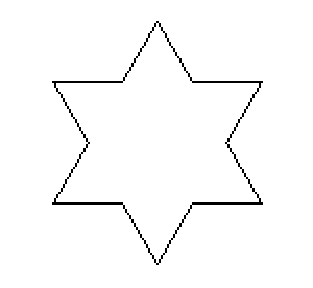
\includegraphics[width=3.5cm, height=3cm]{flocon1.pdf}
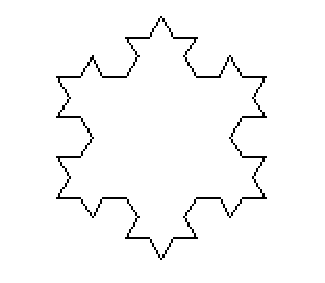
\includegraphics[width=3.5cm, height=3cm]{flocon2.pdf}
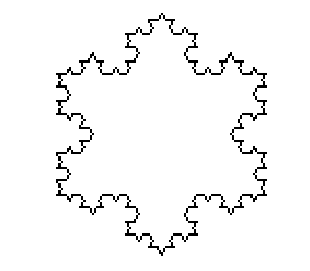
\includegraphics[width=3.5cm, height=3cm]{flocon3.pdf}
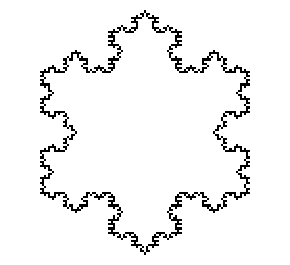
\includegraphics[width=3.5cm, height=3cm]{flocon4.pdf}


\begin{figure}[H]
	\centering
	\caption{Les côtes de la Bretagne}
	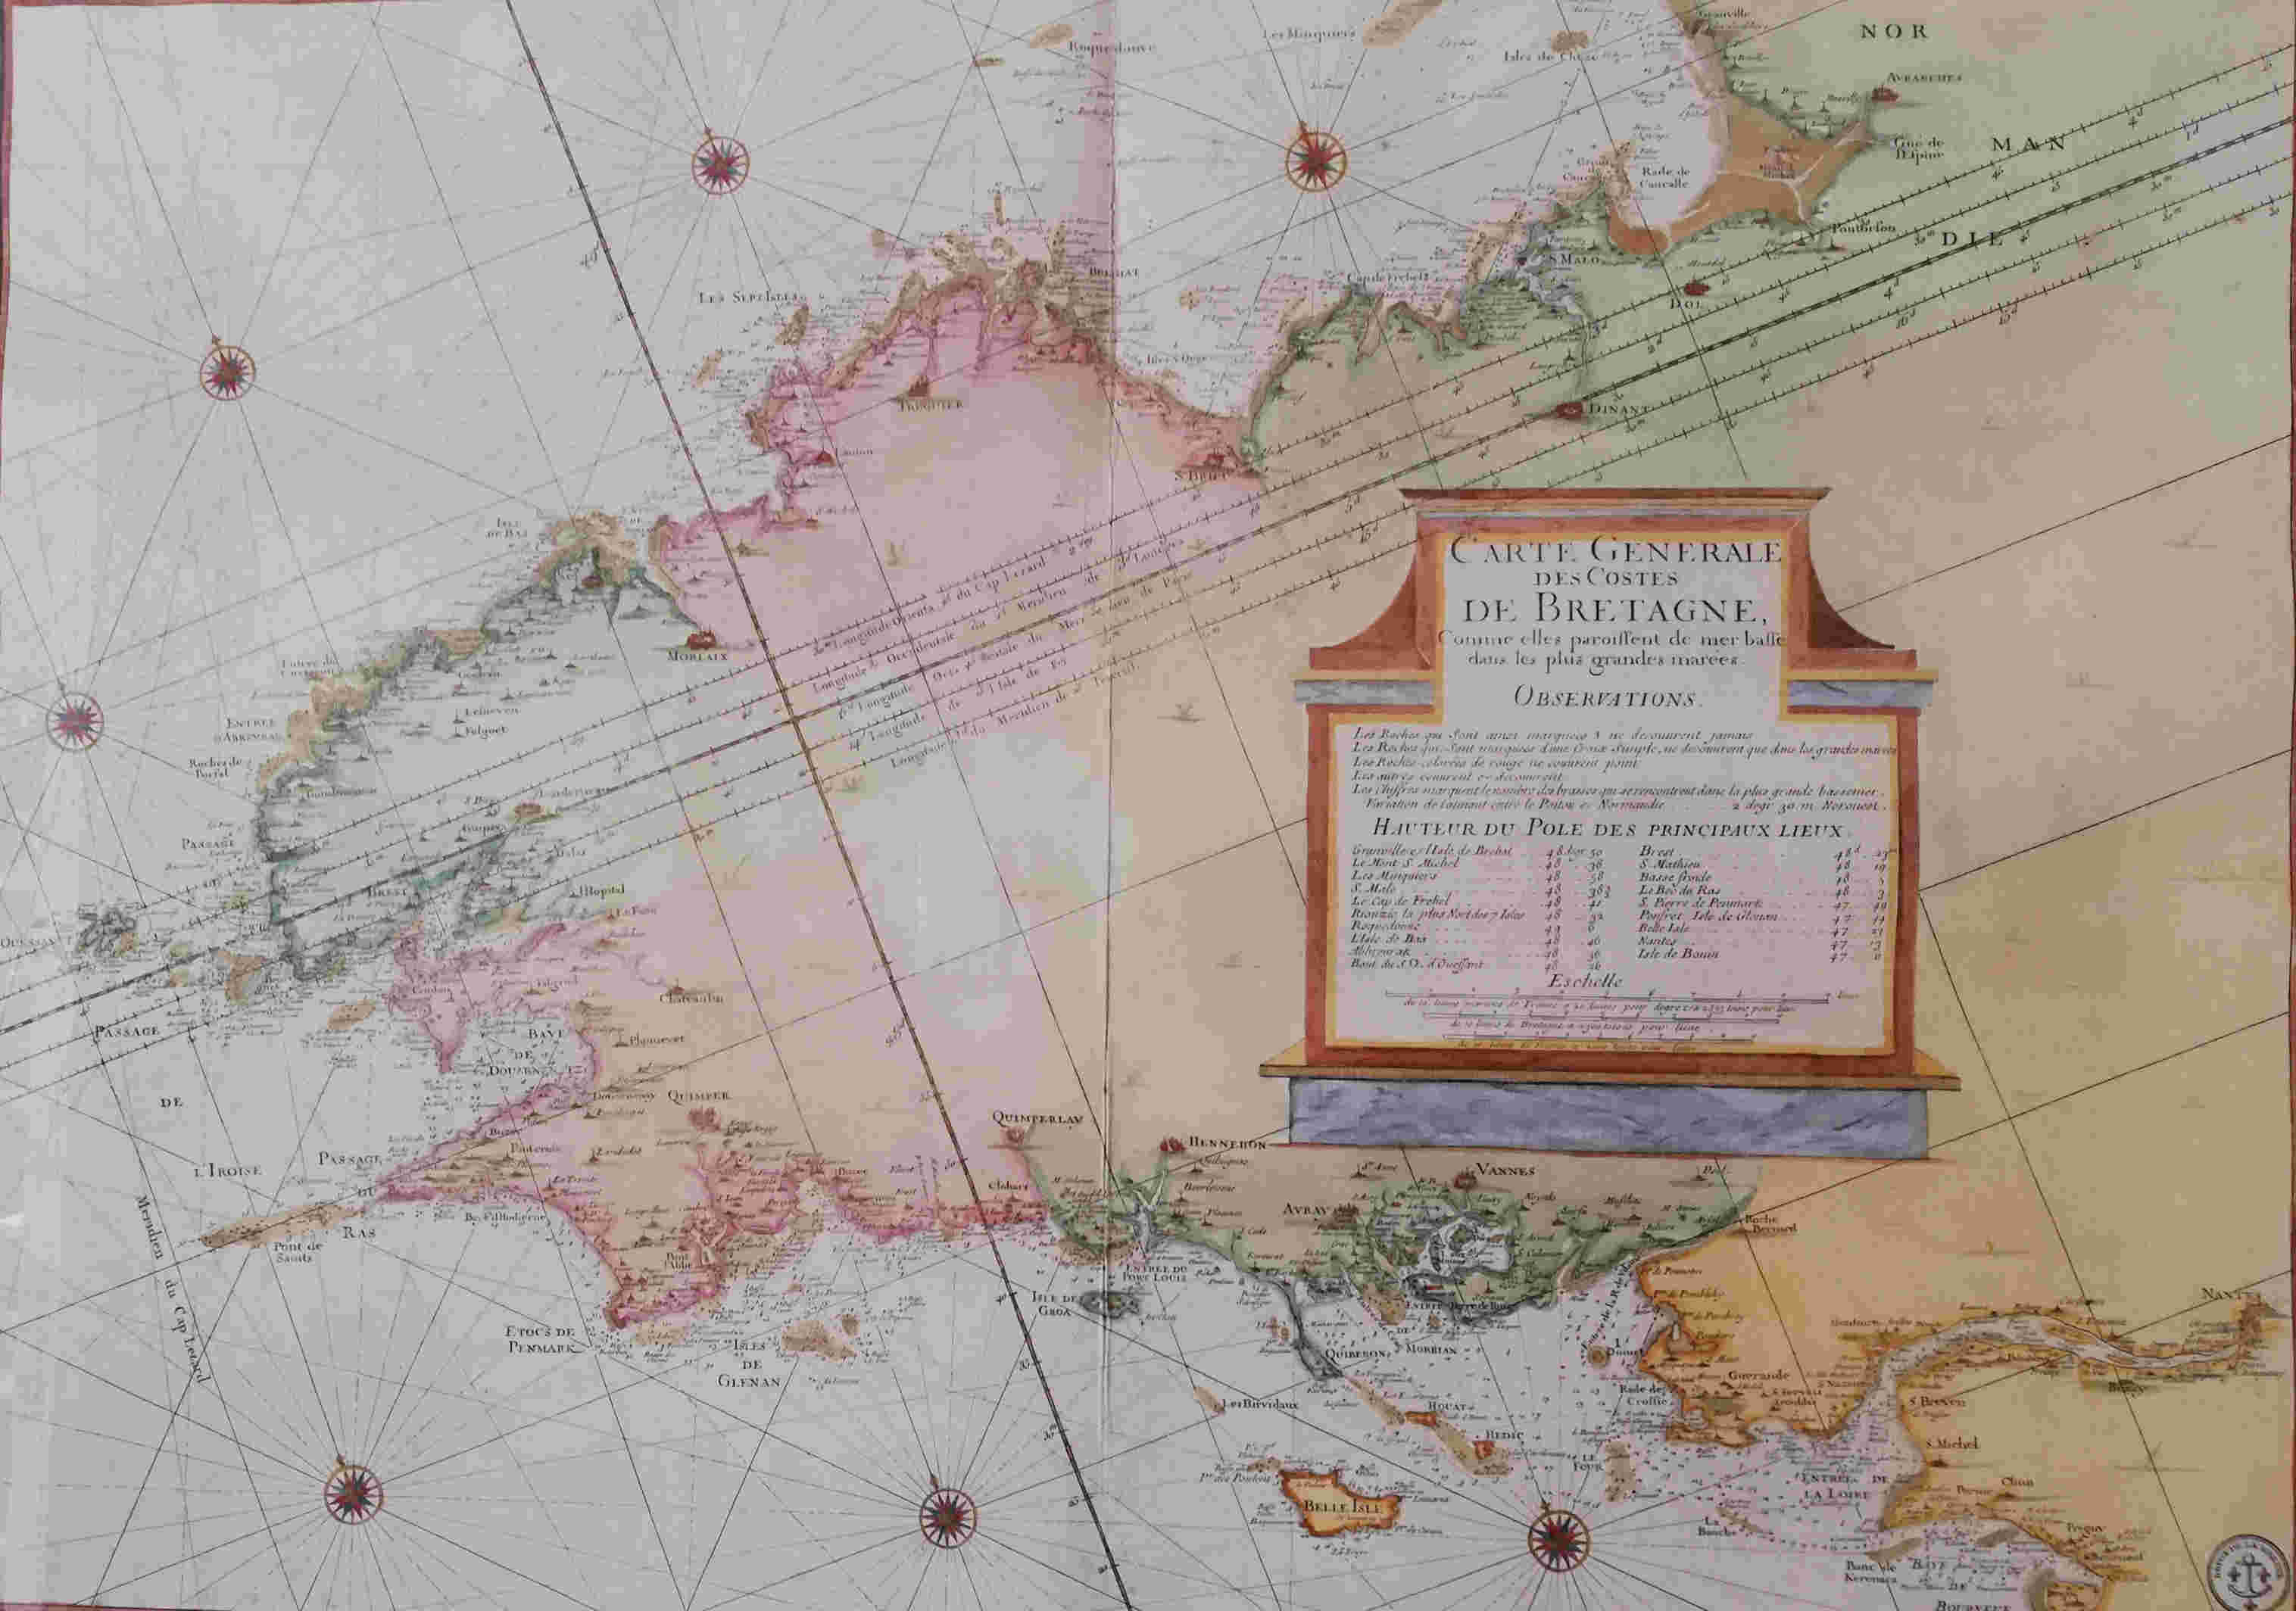
\includegraphics[width=4.0cm]{bretagne3.jpg}
\end{figure}

Les objets fractales ont une propriété surprenante : ils ont une aire finie, mais un périmètre infini.
A l'itération $n$, le périmètre de notre flocon est de $3.(\frac{4}{3})^n$. Et nous avons bien entendu 
$\lim_{n \rightarrow \infty} 3.(\frac{4}{3})^n =\infty $


La longueur des côtes de la Bretagne est-elle aussi infinie ?
\textit{L'Atlantique ronge nos côtes.} \cite{vh}

\subsubsection{L'ensemble de Mandelbrot}
l'ensemble de Mandelbrot est une fractale définie comme l'ensemble des points $c$ 
du plan complexe pour lesquels la suite des nombres complexes définie comme ci-dessous est 
\textbf{bornée}.

$$
\begin{cases}
	z_0=0\\
	z_{n+1}=z_n^2+c
\end{cases}
$$
Voir le bon article \url{https://fr.wikipedia.org/wiki/Ensemble_de_Mandelbrot}

On montre que si la suite des modules des $z_n$ est strictement supérieure à 2 pour un certain indice alors,
cette suite est croissante à partir de cet indice, et elle tend vers l'infini.
Donc notre test d'appartenance à l'ensemble s'arrêtera au-delà de la valeur 2.

Pour estimer la convergence, nous nous arrêterons à la valeur $z_{300}$.
Nous utilisons également l'hypothèse que l'ensemble de Mandelbrot se situe dans le plan complexe
$(-2.00:0.50), (-1.25:1.25)$
\begin{Verbatim}
open Complex ;;   (* {re=2.; im=4.} *)

let appartient c =
	let rec loop n z =
		if (n > 300) then true
		else if ((norm2 z) > 4.) then false
					else loop (n+1) (add c (mul z z)) 
	in loop 0 c  

#load "/home/vincent/.opam/ocaml-base-compiler/lib/graphics/graphics.cma" ;;
#require "graphics" ;; 
open Graphics ;;
Graphics.open_graph " 500x200+0-0" ;;
Graphics.set_window_title "Mandelbrot" ;;
Graphics.set_color Graphics.blue;;

let mandelbrot () =
	for i = (-200) to 50
		do
		  for j=(-125) to 125
			do
			  if (appartient {re=((float_of_int i)/.100.); im=((float_of_int j)/.100.)}) 
			  then plot (200+i) (200+j) 
			done
		done 
\end{Verbatim}

\begin{figure}[H]
	\centering
	\caption{L'ensemble de Mandelbrot}
	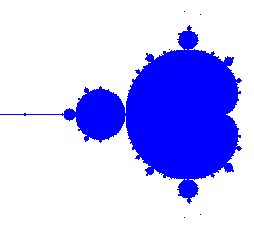
\includegraphics[width=4.0cm]{mandelbrot.png}
\end{figure}

\section{Utilisation de \MF}
\MF\ est un langage créé par D. Knuth \cite{mf}. Il permet le
design de nouvelles fontes de manière très élégante sous forme d'équations.
La programmation se fait principalement de manière déclarative.

Je me suis  amusé ici à créer le symbole  \imp que j'ai souvent
utilisé dans cet article, principalement dans la section sur le $\lambda$-calcul. 

\begin{figure}[H]
	\centering
	\caption{\imp}
	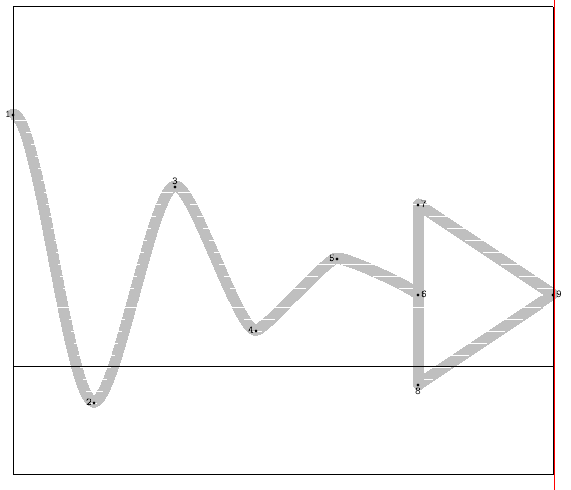
\includegraphics[width=4.0cm]{imp.png}
\end{figure}
Voici le bout de code qui a permis de définir ce symbole:
\begin{Verbatim}
%file name: beta.mf

beginchar("D",15pt#,10pt#,3pt#);
% proportion ligne vs triangle 3/4 1/4
prop:=3/4;

y1=h-d; y2=1/5h-d; y3=4/5h-d; 
y4=2/5h-d; y5=3/5h-d; y6=1/2h-d;  
y7=3/4h-d; y8=1/4h-d; y9=h/2-d;

x1=0; x2=1/5*prop*w; x3=2/5*prop*w;
x4=3/5*prop*w; x5=4/5*prop*w; x6=prop*w;
x7=x8=x6; x9=w;

pickup pencircle scaled 0.3pt;
draw z1{right}..tension 6..z2{right}..tension 5..z3{right}
     ..tension 4..z4{right}..tension 4..z5{right}..tension 3..z6;
draw z7--z8--z9--cycle; 
labels(range 1 thru 9);
endchar;
end
\end{Verbatim}

Nous avons également représenté notre fractale \snow avec le langage \MF .
Cela s'écrit très facilement, car le langage de Knuth permet l'utilisation
de macros récursives.

\begin{Verbatim}
%file name: snow.mf
%mode_setup;
%shape for the character S

i:=1;

def dessine(expr debut, fin) =
z[i]=debut;
z[i+1]=1/3[debut, fin];
z[i+2]= (z[i+1]-z[i]) rotated 60 shifted z[i+1];
z[i+3] = 2/3[debut, fin] ;
z[i+4] = fin ;  
pickup pencircle scaled 0.1pt;
draw z[i]--z[i+1]--z[i+2]--z[i+3]--z[i+4];
i:=i+5;
enddef;

def motif (expr debut, fin, n) =
if (n=1):dessine(debut,fin) else: 
	motif(debut, 1/3[debut,fin], n-1) ;
	motif(1/3[debut,fin],
		(1/3[debut,fin] - debut) rotated 60 shifted (1/3[debut,fin]), n-1) ;
	motif((1/3[debut,fin] - debut) rotated 60 shifted (1/3[debut,fin]),
		(1/3[debut,fin] -debut) shifted (1/3[debut,fin]), n-1) ;
	motif((1/3[debut,fin] - debut) shifted (1/3[debut,fin]), fin, n-1) ;
fi;
enddef;

beginchar("S",15pt#,15pt#,5pt#); "The snowflake" ;
motif((0,0), (w/2,h),4);
motif((w/2,h), (w,0),4);
motif((w,0), (0,0),4);
endchar;
end
\end{Verbatim}

Voici le résultat:
\begin{figure}[H]
	\centering
	\caption{\snow}
	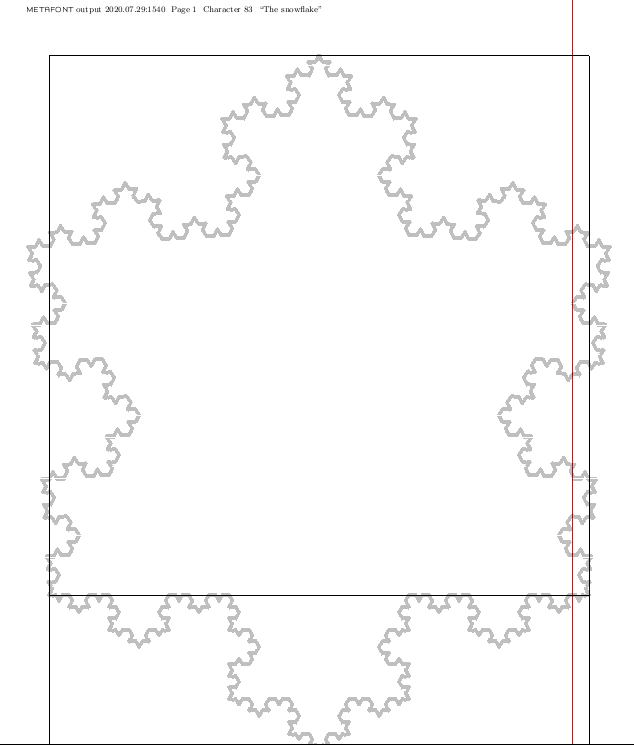
\includegraphics[width=4.0cm]{snow.png}
\end{figure}

\section{The boxes}
Nous avons vu comment représenter un environnement comme une liste
d'associations avec des paires \verb+variable.valeur+.
Une autre méthode est d'utiliser le principe de \textit{box} qui encapsule la
valeur dans une lambda. La \textit{box} est une lambda qui prend une valeur à  sa
création. Puis elle réagit à  deux messages qui permettent respectivement
d'afficher la valeur capturée ou de la modifier avec la procédure \verb+set!+


Voici l'implémentation en Scheme:
\begin{Verbatim}
(define (box value)
  (lambda (msg)
    (case msg
      ("get" value)
      ("set" (lambda (new-value) (set! value new-value))))))

(define (make-box value)
  (box value))

(define maboite (make-box 4))
(maboite "get")
((maboite "set") 5)
\end{Verbatim}

En \textsc{Ocaml}, nous pouvons rédiger le code ci-dessous:
\begin{Verbatim}
exception Erreur

let box value0 =
	let value = ref value0 in
	fun message ->
		match message with
		| "get" -> (fun any -> print_int !value)
		| "set" -> (fun newvalue -> (value := newvalue ; print_int !value ))
		| "reset"-> (fun any -> (value := value0 ; print_int !value))
		| _ -> raise Erreur
		
		
let maboite = box 5 ;;
(maboite "get") 0 ;;
(maboite "set") 1976 ;;
(maboite "get") 0 ;;
(maboite "reset") 0 ;;
\end{Verbatim}

\section{Les modules \textsc{Ocaml}. Modélisation d'un monoïde}
Un monoïde est une structure algébrique qui possède une loi de composition
interne associative et un élément neutre.
Représentons cette structure en \textsc{Ocaml}, en définissant un module.
Nous reprenons ici l'excellent article 
https://blog.derniercri.io/observons-une-premiere-structure-algebrique-appliquee-a-linformatique-le-monoide/
\begin{Verbatim}
module type MONOID =
sig
type t
val ( <+> ) : t -> t -> t
val neutral : t	
end

module String_monoid : MONOID with type t = string  =
struct
type t = string
let ( <+> ) = (^)
let neutral = ""
end

String_monoid.("abc" <+> "def" <+> neutral)
-> String_monoid.t = "abcdef"	
\end{Verbatim}

En algèbre, un morphisme (ou homomorphisme) est une application entre deux structures algébriques
de même espèce.

Pour les  monoïdes, un morphisme est une application 
$f:(M,*,e)\longrightarrow (M',\star ,e')$ , entre deux monoïdes $ (M,*,e)$ et 
$(M',\star , e')$ qui vérifie :
\begin{itemize}
	\item $\forall (g,h)\in M^{2},~f(g*h)=f(g)\star f(h)$
	\item $f(e)=e'$
\end{itemize}
\begin{Verbatim}
#load "Str.cma"

let count  t =  split (regexp " ") t   |> List.length ;;

let pageA = "Hello World "
let pageB = "Foo bar "
let pageC = "O Caml " ;;

count String_monoid.(pageA <+> pageB <+>  pageC) ;;
count(String_monoid.(pageA)) + count(String_monoid.(pageB)) + count(String_monoid.(pageC));;
\end{Verbatim}
Nous avons ici utilisé l'opérateur \verb+|>+ défini comme suit \verb+let ( |> ) x f = f x+

Cette fonction \verb+count+ est ainsi un morphisme entre le monoïde \verb+String_monoid+ et 
le monoïde des entiers (avec $+$ comme fonction de composition interne et $0$
comme élément neutre)
\section{Machine Learning and Neural Networks}

\subsection{Introduction}

Nous implémentons en R un réseau de neurones réduit à sa plus simple expression.
Il n'aura que deux couches de neurones.
Le langage R est ici commode pour ses opérations natives sur les matrices.
Nous pourrons voir ensuite comme transposer ce code en \textsc{Ocaml}.

Nous entraînerons notre NN sur la base du jeu de test MNIST.
Le  "training set" contient 60000 exemples, et le "test set" 10000 exemples.
Nous pourrons nous documenter plus précisément avec l'excellent ouvrage de François Chollet \cite{deepR}.

\subsection{Un peu de théorie}

Soit les 150 observations suivantes représentées par la matrice $X_{150,784}$ (ou tensor 2 dimensions) comprenant 150 lignes pour les 150 observations et 784 colonnes pour les 784 features des observations.

2 matrices de poids $W^1_{32,150}$ et $W^2_{10,150}$ sont utilisées.

\begin{itemize}
	\item 1er layer de 32 neurones
	\item 2nd layer de 10 neurones
\end{itemize}

La sortie $OUTPUT_{150,10}$ est une matrice de 150 lignes avec les 10 colonnes représentant 
les 10 features que l'on cherche à reconnaître.

Voici le schéma simplifié du NN à 2 couches:

$$
X \longrightarrow \otimes W^1 \rightarrow  Z^1 \rightarrow \sigma \rightarrow LAYER^1 \longrightarrow
\otimes W^2 
\rightarrow Z^2 
\rightarrow 
\sigma 
\rightarrow \hat{Y} 
>> LOSS(\hat{Y}, Y)
$$

\subsection{Calcul matriciel}

Cela donne le calcul matriciel ci-dessous:
\begin{footnotesize}
\begin{align*}
\begin{pmatrix}
x_{1,1} & x_{1,2} & \cdots & x_{1,784} \\
x_{2,1} & x_{2,2} & \cdots & x_{2,784} \\
\vdots  & \vdots  & \ddots & \vdots  \\
x_{150,1} & x_{150,2} & \cdots & x_{150,784} 
\end{pmatrix}
\times
\begin{pmatrix}caml
w^1_{1,1} & w^1_{1,2} & \cdots & w^1_{1,32} \\
w^1_{2,1} & w^1_{2,2} & \cdots & w^1_{2,32} \\
\vdots  & \vdots  & \ddots & \vdots  \\
w^1_{784,1} & w^1_{784,2} & \cdots & w^1_{784,32} 
\end{pmatrix}
&= 
\begin{pmatrix}
z^1_{1,1} & z^1_{1,2} & \cdots & z^1_{1,32} \\
z^1_{2,1} & z^1_{2,2} & \cdots & z^1_{2,32} \\
\vdots  & \vdots  & \ddots & \vdots  \\
z^1_{150,1} & z^1_{150,2} & \cdots & z^1_{150,32} 
\end{pmatrix}
\\
\sigma(
\begin{pmatrix}
z^1_{1,1} & z^1_{1,2} & \cdots & z^1_{1,32} \\
z^1_{2,1} & z^1_{2,2} & \cdots & z^1_{2,32} \\
\vdots  & \vdots  & \ddots & \vdots  \\
z^1_{150,1} & z^1_{150,2} & \cdots & z^1_{150,32} 
\end{pmatrix}
)
\times
\begin{pmatrix}
w^2_{1,1} & w^2_{1,2} & \cdots & w^2_{1,10} \\
w^2_{2,1} & w^2_{2,2} & \cdots & w^2_{2,n} \\
\vdots  & \vdots  & \ddots & \vdots  \\
w^2_{32,1} & w^2_{32,2} & \cdots & w^2_{32,10} 
\end{pmatrix}
&= 
\begin{pmatrix}
z^2_{1,1} & z^2_{1,2} & \cdots & z^2_{1,10} \\
z^2_{2,1} & z^2_{2,2} & \cdots & z^2_{2,10} \\
\vdots  & \vdots  & \ddots & \vdots  \\
z^2_{150,1} & z^2_{150,2} & \cdots & z^2_{150,10} 
\end{pmatrix}
\\
\sigma(
\begin{pmatrix}
z^2_{1,1} & z^2_{1,2} & \cdots & z^2_{1,10} \\
z^2_{2,1} & z^2_{2,2} & \cdots & z^2_{2,10} \\
\vdots  & \vdots  & \ddots & \vdots  \\
z^2_{150,1} & z^2_{150,2} & \cdots & z^2_{150,10}
\end{pmatrix}
)
&=
\begin{pmatrix}
\hat{y}_{1,1} & \hat{y}_{1,2} & \cdots & \hat{y}_{1,10} \\
\hat{y}_{2,1} & \hat{y}_{2,2} & \cdots & \hat{y}_{2,10} \\
\vdots  & \vdots  & \ddots & \vdots  \\
\hat{y}_{150,1} & \hat{y}_{150,2} & \cdots & \hat{y}_{150,10} 
\end{pmatrix}
\end{align*}
\begin{align*}
LOSS(Y, \hat{Y}) &= \sum (
\begin{pmatrix}
\hat{y}_{1,1} & \hat{y}_{1,2} & \cdots & \hat{y}_{1,10} \\
\hat{y}_{2,1} & \hat{y}_{2,2} & \cdots & \hat{y}_{2,10} \\
\vdots  & \vdots  & \ddots & \vdots  \\
\hat{y}_{150,1} & \hat{y}_{150,2} & \cdots & \hat{y}_{150,10} 
\end{pmatrix}
-
\begin{pmatrix}
y_{1,1} & y_{1,2} & \cdots & y_{1,10} \\
y_{2,1} & y_{2,2} & \cdots & y_{2,10} \\
\vdots  & \vdots  & \ddots & \vdots  \\
y_{150,1} & y_{150,2} & \cdots & y_{150,10} 
\end{pmatrix}
)^2
\end{align*}

\begin{align*}
Z_1 &= X.W_1 \\
LAYER_1 &= \sigma (Z_1) \\
Z_2 &= LAYER_1 * W_2 \\
\hat{Y} &= \sigma (Z_2) \\
LOSS &= (\hat{Y} -Y)^2  
\end{align*}
\end{footnotesize}

Calculons la dérivée de la fonction $LOSS$ en fonction de $W^1$

\begin{align*}
 \frac{\delta LOSS}{\delta W_1} &=\frac{\delta LOSS}{\delta \hat{Y}} . \frac{\delta \hat{Y}}{\delta Z_2}. \frac{\delta Z_2}{\delta LAYER_1 }.\frac{\delta LAYER_1}{\delta Z_1 }. \frac{\delta Z_1}{\delta W_1 } \\ 
  &= 2(\hat{Y}-Y) . \sigma ^\prime (Z_2) . W_2 . \sigma ^\prime (Z_1). X
\end{align*}

$2(\hat{Y}-Y)$ est une matrice de dimension $(150, 10)$

$\sigma ^\prime (Z_2)$ est une matrice de dimension $(150,10)$

$W_2$ est une matrice de dimension $(32,10)$

$\sigma ^\prime (Z_1)$ est une matrice de dimension $(150,32)$

$X$ est une matrice de dimension $(150,784)$

Le calcul matriciel qui sera fait est $t(X)* \{ (2(\hat{Y}-Y) . \sigma ^\prime (Z^2) * t(W^2). \sigma ^\prime (Z^1)\}$, où $*$ est le produit matriciel et $.$ le produit d'Hadamard.
Le résultat donne une matrice de dimension $(784,32)$ qui est de même dimension que $W_1$
\begin{align*}
t(150,784)* \{(150,10).(150,10)*t(32,10).(150,32))\} &= (784,150) * \{(150,10)*(10,32).(150,32)\}\\ 
&= (784,150)*(150,32) \\
&=(784,32)
\end{align*}

 
\subsection{Fonctions d'activation}

Pour la fonction d'activation, ici appelée $\sigma$, nous utiliserons pour la première couche la fonction $relu(x) = max(o,x)$

Pour la seconde couche, nous utiliserons la fonction sigmoid $f(x)= \frac{1}{1+e^{-x}}$

\begin{figure}[H]
\centering
\caption{La fonction sigmoid}
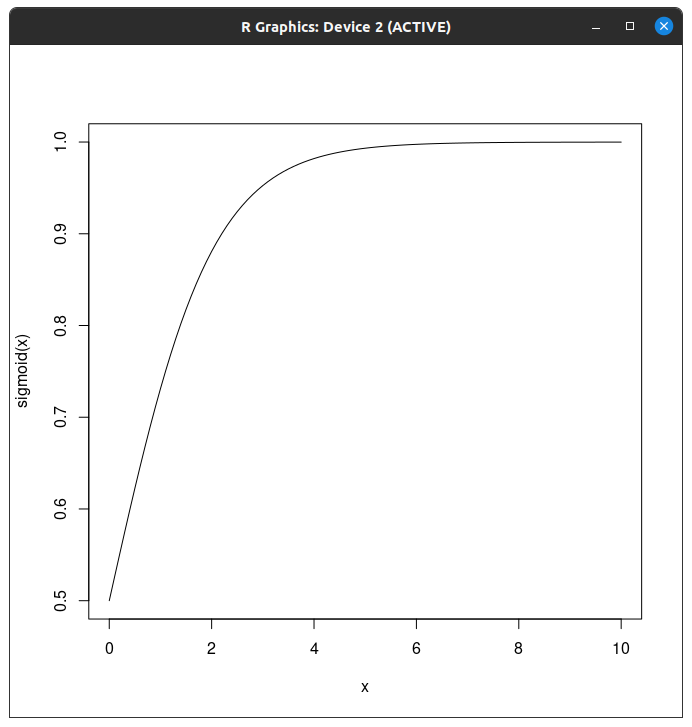
\includegraphics[width=5cm, height=5cm]{sigmoid}
\end{figure}

Voici le code en R:

\begin{Verbatim}
# the activation function
sigmoid <- function(x) {
	1.0 / (1.0 + exp(-x))
}

x=seq(0,10,0.1)
plot(x, sigmoid(x), type="l") 

# the derivative of the activation function
sigmoid_derivative <- function(x) {
	sigmoid(x) * (1.0 - sigmoid(x))
}
\end{Verbatim}


Calculons la dérivée de la fonction $LOSS$ en fonction de $W^2$ 

\begin{align}
\frac{\delta LOSS}{\delta W_2} & =\frac{\delta LOSS}{\delta \hat{Y}} . \frac{\delta \hat{Y}}{\delta Z_2}. \frac{\delta Z_2}{\delta W_2 } \\
 &= 2(\hat{Y}-Y) . \sigma ^\prime (Z_2) . LAYER_1 
\end{align}

$2(\hat{Y}-Y)$ est une matrice de dimension $(150, 10)$

$\sigma ^\prime (Z_2)$ est une matrice de dimension $(150,10)$

$LAYER_1$ est une matrice de dimension $(150,32)$

Le calcul matriciel qui sera fait est $t(LAYER_1)* (2(\hat{Y}-Y) . \sigma ^\prime (Z_2))$, où $*$ est le produit matriciel et $.$ le produit d'Hadamard.
Le résultat donne une matrice de dimension $(32,10)$ qui est de même dimension que $W_2$
$$
t(150,32) * (150,10).(150.10) = (32,150)*(150,10)=(32,10)
$$


\section{Les nombres premiers. L'algorithme RSA}

\begin{itemize}
	\item Le crible d'Erathostène (\textgreek{'Eratosjénhs}) 
	\item Leur répartition
	\item Les nombres premiers jumeaux
	\item La constante de Brun 
	\item La fonction zêta
	\item Le produit eulérien et sa convergence avec la suite harmonique
	\item Le petit théorème de Fermat
	\item La fonction \textit{indicatrice} d'Euler
	\item L'algorithme RSA
\end{itemize}

\subsubsection{Le crible}
\begin{Verbatim}
type 'a stream = Cons of 'a * (unit -> 'a stream) ;;
let hd (Cons (h, _)) = h ;;
let tl (Cons (_, tf)) = tf () ;;

let rec take n s =
	if n=0 then []
	else hd s :: take (n-1) (tl s) 

let rec entiers x = Cons(x, fun() -> entiers(x+1)) 

let rec filtre m (Cons(x,l)) =
	if x mod m = 0 then filtre m (l()) 
	else Cons(x, fun() -> (filtre m (l()))) 

let rec crible (Cons(x,l)) = Cons(x, fun()-> crible(filtre x (l())))

let premiers = crible(entiers 2) ;;
\end{Verbatim}
\begin{Verbatim}
utop # take 100 premiers ;;
- : int list =
[2; 3; 5; 7; 11; 13; 17; 19; 23; 29; 31; 37; 41; 43; 47; 53; 59; 61; 67; 71;
 73; 79; 83; 89; 97; 101; 103; 107; 109; 113; 127; 131; 137; 139; 149; 151;
 157; 163; 167; 173; 179; 181; 191; 193; 197; 199; 211; 223; 227; 229; 233;
 239; 241; 251; 257; 263; 269; 271; 277; 281; 283; 293; 307; 311; 313; 317;
 331; 337; 347; 349; 353; 359; 367; 373; 379; 383; 389; 397; 401; 409; 419;
 421; 431; 433; 439; 443; 449; 457; 461; 463; 467; 479; 487; 491; 499; 503;
 509; 521; 523; 541]
\end{Verbatim}

\subsubsection{Le produit d'Euler aka le produit eulérien}
La fonction zêta est égale au produit eulérien
\[ \zeta(s) = \sum_{n=1}^{\infty} \frac{1}{n^s} = \prod_{i=1}^\infty \frac{1}{1-p_i^{-s}} = \prod_{i=1}^\infty \frac{p_i^s}{p_i^s-1} \]

Exemple pour $s=1$ avec la suite harmonique
$$
\begin{array}{ccc}
1+ \frac{1}{2} + \frac{1}{3} + \frac{1}{4} + \frac{1}{5} +...  &=  \frac{1}{1-\frac{1}{2}} .\frac{1}{1-\frac{1}{3}}.\frac{1}{1-\frac{1}{5}}.\frac{1}{1-\frac{1}{7}}. (...) \\[\bigskipamount]
&= \frac{2.3.5.7.11.13.17.19...}{1.2.4.6.10.12.16.18...} 
\end{array}
$$

Démontrons cela
\[\zeta(1) = 1+ \frac{1}{2} + \frac{1}{3} + \frac{1}{4} + \frac{1}{5}+ \frac{1}{6}+ \frac{1}{7} +  \frac{1}{8} +... \]

Divisons par 2
\[ \frac{\zeta(1)}{2} = \frac{1}{2}+\frac{1}{4}+\frac{1}{6}+\frac{1}{8}+\frac{1}{10}+\frac{1}{12} + \frac{1}{14}+ \frac{1}{16}+... \]
 
La différence de ces 2 équations donne:
\[ \zeta(1).(1-\frac{1}{2}) = 1 + \frac{1}{3}+\frac{1}{5}+\frac{1}{7}+\frac{1}{9}+\frac{1}{11}+\frac{1}{13}+ ... \]

Divisons par 3
\[ \frac{1}{3}.(1-\frac{1}{2}).\zeta(1) = \frac{1}{3} + \frac{1}{9}+\frac{1}{15}+\frac{1}{21}+\frac{1}{27}+ \frac{1}{33}+ \frac{1}{39}+... \]

La différence donne:
\[ (1-\frac{1}{3}).(1-\frac{1}{2}).\zeta(1) = 1 + \frac{1}{5} + \frac{1}{7}+\frac{1}{11}+\frac{1}{13}+ ... \]

Divisons par 5
\[ \frac{1}{5}.(1-\frac{1}{3}).(1-\frac{1}{2}).\zeta(1) =    \frac{1}{5} + \frac{1}{25}+\frac{1}{35}+\frac{1}{55}+ ... \]

La différence donne:
\[(1-\frac{1}{5}).(1-\frac{1}{3}).(1-\frac{1}{2}).\zeta(1) = 1 + \frac{1}{7}+\frac{1}{11}+\frac{1}{13}+... \]

Nous pouvons poursuivre sur le principe du crible d'Erathostène
\[ \ldots(1-\frac{1}{5}).(1-\frac{1}{3}).(1-\frac{1}{2}).\zeta(1) = 1 \]

D'où :
$$
\begin{array}{ccc}
\zeta(1) &=& \frac{1}{(1-\frac{1}{2}).(1-\frac{1}{3}).(1-\frac{1}{5})\ldots} \\[\bigskipamount]
\zeta(1) &=& \frac{1}{\frac{1}{2}.\frac{2}{3}.\frac{4}{5}\ldots} 		\\[\bigskipamount]
\zeta(1) &=&  \frac{2.3.5.7.11.13.17.19...}{1.2.4.6.10.12.16.18...} \\[\bigskipamount]
\end{array}
$$

Le numérateur est le produit de l'ensemble des nombres premiers.
Le dénominateur est le produit de l'ensemble des nombres premiers moins 1.


Exemple pour $s=2$ avec la suite carrée
\[ 1+ \frac{1}{4} + \frac{1}{9} + \frac{1}{16} + ...  =  \frac{1}{1-\frac{1}{4}} .\frac{1}{1-\frac{1}{9}}.\frac{1}{1-\frac{1}{25}}.\frac{1}{1-\frac{1}{49}}. (...) \]



\subsubsection{Les nombres premiers jumeaux et la constante de Brun}
La somme inverse des nombres premiers jumeaux. Il y en aurait une infinité. Cependant, cette somme
 converge vers la constante de Brun.



\begin{align*}
   Brun &= (\frac{1}{3} + \frac{1}{5}) + (\frac{1}{5} + \frac{1}{7}) + (\frac{1}{11} + \frac{1}{13}) + (\frac{1}{17} + \frac{1}{19}) + (\frac{1}{29} + \frac{1}{31}) +\  ...  \\
   Brun &\approx 1,90216
\end{align*}


\begin{Verbatim}
let rec filtre_jumeaux = function
 | Cons(x,l) -> if (hd (l()) = (x+2)) then 
                  Cons(x, fun() -> Cons ((hd (l())) , (fun() ->  (filtre_jumeaux  (l())))))
                else filtre_jumeaux (l()) ;;

take 100 (filtre_jumeaux premiers) ;;

let rec inverse (Cons(x,l)) = Cons(1. /. float_of_int x, fun() -> inverse(l())) ;;

let inverse_jumeaux = inverse (filtre_jumeaux premiers) ;;

let rec somme n s =
if n=0 then 0.
else hd s +. somme (n-1) (tl s) ;;

somme 10000 inverse_jumeaux ;;
 \end{Verbatim}

 Avec les 10000 premières paires, nous sommes encore loin de $1,90216$\dots

\subsubsection{Le petit théorème de Fermat}
Si $p$ est premier et si $a$ n’est pas un multiple de $p$, alors $a^{p−1}≡1  \mod p$

\subsubsection{Le théorème d'Euler}
L'indicatrice d'Euler est une fonction, qui à tout entier naturel $n$ non nul associe
 le nombre d'entiers compris entre 1 et $n$ et premiers avec $n$. Cette fonction est nommée en anglais
 \textit{Euler's totient function}
$$
\begin{array}{ccccl}
  \varphi & : & \mathbb{N}^* & \longrightarrow & \mathbb{N}^* \\
   & & n& \longmapsto &\mathrm{card}\{ m \in \mathbb{N}^* ~|~m\le n~  \text{et}~m~\mathrm{premier~avec}~n \}
\end{array}
$$


Le théorème d'Euler nous dit que $ a^{\varphi (n)} \equiv 1 \mod n $, si $a$ est un entier premier à $n$.
C'est une généralisation du petit théorème de Fermat.

\subsubsection{Le théorème de Bezout}
$$ \forall x,y \in \mathbb{N},\ \exists u , v \in \mathbb{Z}\ \mathrm{tel\ que}\ ux+vy=\mathrm{pgcd}(x,y) $$

\subsubsection{L'inverse modulaire}
Avec $x$ et $n$ premiers entre eux, en prenant $u$ et $v$ dans $\mathbb{Z}$ tels que
$ux+vn=1$, on a : 
\begin{align*} 
  u.x &\equiv 1  \mod n  \\
  u &\equiv x^{-1} \mod n 
\end{align*}

\subsubsection{L'algorithme RSA}

Soient $p>1$ et $q>1$ deux nombres premiers distincts, $n=pq$ leur produit,
 $e$ un nombre premier avec 
$\varphi(n) = (p−1)(q−1)$ et $d = e^{−1} \mod{(p−1)(q−1)}$.

Pour tout entier positif $m<n$, on a $m^{ed} ≡ m \mod n$

La clé publique  est le couple $P=(n,e)$,
la clé secrète est le couple $S=(n,d)$.

\textit{Raisonnement:}

$ed≡1 \mod (p−1)(q−1)$, donc il existe $k$ tel que $ed=1+k(p−1)(q−1)$.

Si $m$ n’est pas multiple de $p$ ni de $q$, 
d’après le petit théorème de Fermat,
$$
\begin{cases}
  m^{ed}= m^{1+k(p−1)(q−1)} = m (m^{p-1})^{k(q-1)} \equiv m \mod p \\ 
 
  m^{ed}= m^{1+k(p−1)(q−1)} = m (m^{q-1})^{k(q-1)} \equiv m \mod q
\end{cases}
$$
et si $m$ est un multiple de $p$, $m≡0 \mod p$ et $m^{ed}≡0 \mod p$ (de même avec $q$).

 L’entier $u^{ed}−m$ est donc un multiple de $p$ et de $q$, qui sont premiers distincts, 
 donc un multiple de leur produit $pq=n$

 Donc, pour tout entier $m, m^{ed} ≡ m \mod n$

 \subsubsection{Le code}
 \begin{Verbatim}
open List
open Random 

let p = 61 and q = 53 ;;
let n = p*q ;;
let phi = (p-1)*(q-1) ;; (* phi=3233 *)
let m = 65 ;;

let rec pgcd a b =
  if b = 0 then a 
  else pgcd b (a mod b)

let rec calcule_e p q =
  let e = Random.int ((p-1)*(q-1))
    in if pgcd e ((p-1)*(q-1)) = 1 then e
      else calcule_e p q  

let rec euclide a b = 
  if b = 0 then ( a , 1 , 0 ) 
    else 
    begin
        let (d', u', v') = euclide b (a mod b)
        in (d', v', u' - (a / b) * v' )
    end

let calcule_d p q e =
    let(_, u ,_) = euclide e (( p-1)*(q-1)) in
      u mod ((p-1)*(q-1))

let rec pow a m = function
  | 0 -> 1 mod m
  | 1 -> a mod m
  | n -> 
    let b = pow a m (n / 2) in
    b * b * (if n mod 2 = 0 then 1 else a) mod m
  ;;    

let e = calcule_e p q  ;;
let d = calcule_d p q e ;;

crypt (crypt m e n) d n;;

let factor n =
  let rec aux n k l =
    if n < k/2 then l
    else if (n mod k) = 0 then aux (n/k) k (k::l)
    else if (k=2) then aux n 3 l 
    else aux n (k+2) l
in rev (aux n 2 [])
\end{Verbatim}

 \section{Approximation du nombre $\pi$ }

\begin{center}
	\begin{tabular}{ccccccccccc}
		Que & j'& aime & à & faire & connaître & ce & nombre & utile & aux & sages. \\
		3,   & 1 &  4   & 1 &  5    &  9        & 2  &  6     &  5    & 3   & 5 \\ 
	\end{tabular}	
\end{center}


Cherchons à approcher $\pi$ par cinq méthodes :
\begin{itemize}
	\item La loi des grands nombres. 
	Nous faisons ici un tirage aléatoire de coordonnées $(x,y)$ avec $x$ et $y$ compris entre $-1$ et $1$.
	Il y a  $\pi$ chances sur 4 que le tirage tombe dans le cercle de rayon 1. 
		
	\item La série alternée de Leibniz 
	\[ \sum_{n=0}^\infty \frac{(-1)^n}{2n+1} = \frac{1}{1} -\frac{1}{3}+\frac{1}{5}-\frac{1}{7}+\frac{1}{9} - \dots = \frac{\pi}{4}  \]
	
	\item Le calcul numérique de l'intégrale 
	$$\int_0^1 \frac{1}{1+x^2} dx$$
	
	\item  Le produit de Wallis 
	\[ \pi /2 = \frac{2.2.4.4.6.6.8.8.10.10. ...} {1.3.3.5.5.7.7.9.9.11. ...}\]
	
	Ce produit s'écrira mieux sous la forme:
	\[ ( \frac{2}{1}.\frac{2}{3} ) . (\frac{4}{2}.\frac{4}{5} ).(\frac{6}{5}.\frac{6}{7} ).(\frac{8}{7}.\frac{8}{9} ) . ...  =  \prod_{n=1}^\infty \frac{2n.2n}{(2n-1).(2n+1)} = \prod_{n=1}^\infty \frac{4n^2}{4n^2-1}\]
	
	\item Les périmètres des polygones réguliers inscrits et circonscrits au cercle 
	\begin{figure}[H]
		\centering
		\usetikzlibrary{shapes.geometric}
		\begin{tikzpicture}
			\foreach \a in {3,...,7}{
			\draw[blue] (\a*3,0) circle(1cm);
			\node[regular polygon, regular polygon sides=\a, minimum size=2cm, draw] at (\a*3,0) {};
			\tikzmath{\x = {28.45*2/cos(deg(3.14/ \a)}; }
			\node[regular polygon, regular polygon sides=\a, minimum size=\x, draw] at (\a*3,0) {};
			}
	
		\end{tikzpicture}
		\end{figure}
	
\end{itemize}

\subsection{La méthode des polygones}	
Pour calculer la valeur de $\pi$, il suffit de calculer pour $n$ suffisament grand
les périmètres des polygones réguliers de $n$ côtés inscrits et circonscrits à un cercle de diamètre
$2R=1$. 
Nous nous reférerons à l'excellent ouvrage \cite{gb}.
Cette approche est appelée en anglais \textit{the method of exhaustion}.


Le périmètre du polygone inscrit sera nommé $p_n$. Le périmètre du polygone circonscrit
sera $p'_n$. Comme $p_n < 2\pi R < p'_n$, on aura $p_n < \pi < p'_n$.
Nous obtiendrons alors deux valeurs approchées de $\pi$, l'une par défaut, l'autre par excès.

\subsubsection{Calcul de $p_{2n}$ en fonction de $p_n$}

Nous rappelons les deux définitions suivantes :
\begin{definition}
	Le rayon du polygone est le rayon du cercle circonscrit. 
\end{definition}

\begin{definition}
	L'apothème du polygone est le rayon du cercle inscrit. 
\end{definition}
Nous pouvons ainsi exprimer l'apothème en fonction du rayon par la formule $a = r \cos (\frac{\pi}{n}) $ où
$n$ est le nombre de côté du polygone.


Soit $AB = c_n$ le côté du polygone régulier inscrit et $OH=a_n$ son apothème. 

$C$ est le milieu de l'arc $AB$. On a $AC=c_{2n}$ 


\begin{figure}[H]
	\centering
	\begin{tikzpicture}
		\draw (0,0) -- (2,0) ;
		\draw (0,0) -- (-2,0) ;
		\draw (0,0) circle (2) ;
	
		\draw (45:2) node[right]{$A$} ;
		\draw (-45:2) node[right]{$B$} ;
		\draw ({sqrt(2)},0) node[below right]{$H$} ;

		\draw (0,0) -- (45:2) ;
		\draw (-2,0) -- (45:2) ;
		\draw (2,0) -- (45:2) ;
		\draw (45:2) -- (-45:2) node[near start] {$c_{2n}$} ;
		\draw (0,0) -- ({sqrt(2)},0) node[midway, below] {$a_{n}$} ;
	
		\draw (0,0) node[below]{$O$} ;
		\draw (2,0) node[right]{$C$} ;
		\draw (-2,0) node[left]{$C'$} ;
	\end{tikzpicture}
	\end{figure}

Dans le triangle rectangle $ACC'$ : 

\begin{align*}
AC^2 &= CC'.CH = CC' (OC - OH) \\
\Leftrightarrow  c_{2n}^2 &= 2R -(R-a_n)
\end{align*}


Or
\begin{align*}
OH &= \sqrt{OA²-AH²} \\
\Leftrightarrow  a_n &= \sqrt{R²-\frac{c_n^2}{4}}
\end{align*}

Donc
$$ c_{2n}^2 = R (2R-\sqrt{4R^2 - c_n^2}) $$
Comme $ c_n = \frac{p_n}{n} $, on obtient :
$$ \frac{p_{2n}^2}{4n^2}=R(2R-\sqrt{4R^2-\frac{p^2}{n^2}}) $$
Soit pour $2R=1$
$$ \boxed{ p_{2n}^2 = 2n (n - \sqrt{n^2-p_n^2}) } $$

En partant d'un carré inscrit $(n=4)$, nous avons $c_4=\frac{\sqrt{2}}{2}$ et donc 
nous pouvons calculer les valeurs de $p_8, p_{16}, p_{32}, \dots$

\subsubsection{Calcul de $p'_n$ en fonction de $p_n$}
Les polygones inscrits et cirsconscrits étant deux polygones semblables, nous avons :
\begin{align*}
\frac{p'_n}{p_n} &= \frac{R}{a_n} \\
\Leftrightarrow  p'_n &= p_n . \frac{R}{a_n} \\
\Leftrightarrow  p'_n &= p_n . \frac{2R}{\sqrt{4R^2 - c_n^2}} \\
\Leftrightarrow  p'_n &= \frac{2nRp_n}{\sqrt{4n^2 R^2 - p_n^2}} 
\end{align*}

Soit pour $2R=1$
$$ \boxed{ p'_n = \frac{np_n}{\sqrt{n^2-p_n^2}} } $$

\begin{tikzpicture}

	\tikzmath{\n = 4; 
			  \p4 = {2*sqrt(2)};
			  \q4 = {\n * \p4 / sqrt(\n^2 - \p4^2)} ;
			  \p8 = {sqrt(2*\n *(\n - sqrt(\n^2 - \p4^2)))} ;
			  \n = 8;
			  \q8 = {\n * \p8 / sqrt(\n^2 - \p8^2)} ;
			  \p16 = {sqrt(2*\n *(\n - sqrt(\n^2 - \p8^2)))} ;
			  \n = 16;
			  \q16 = {\n * \p16 / sqrt(\n^2 - \p16^2)} ;
			  \p32 = {sqrt(2*\n *(\n - sqrt(\n^2 - \p16^2)))} ;
			  \n = 32;
			  \q32 = {\n * \p32 / sqrt(\n^2 - \p32^2)} ;
			  \p64 = {sqrt(2*\n *(\n - sqrt(\n^2 - \p32^2)))} ;
			  \n = 64;
			  \q64 = {\n * \p64 / sqrt(\n^2 - \p64^2)} ;
		%	  \p128 = {sqrt(2*\n *(\n - sqrt(\n^2 - \p64^2)))} ;
		%	  \n = 128;
		%	  \q128 = {\n * \p128 / sqrt(\n^2 - \p128^2)} ;
	        }
	\node[draw,text width=15cm] at(0,0){Les valeurs approchées de $\pi$ par défaut, et par excès en fonction
	du nombre $n$ de côtés :\\
	 $ n=4 \rightarrow \p4 < \pi < \q4 $ \\
	 $ n=8 \rightarrow \p8 < \pi < \q8 $  \\
	 $ n=16 \rightarrow \p16 < \pi < \q16 $ \\
	 $ n=32 \rightarrow \p32 < \pi < \q32 $  \\
	 $ n=64 \rightarrow \p64 < \pi < \q64 $ \\
	% $ n=128 \rightarrow \p128 < \q128 $ \\
	 	 }  ;
\end{tikzpicture}


\vspace{1cm}
Depuis la formule $  p_{2n}^2 = 2n (n - \sqrt{n^2-p_n^2})  $ et sachant que $p_n = n.c_n$, 
nous pouvons en déduire :
$$ c_{2n} = \sqrt{2-\sqrt{4-c_n^2}} $$

Pour un carré de rayon $1$, nous avons $c_4=\sqrt{2}$. Ainsi $c_8= \sqrt{2-\sqrt{2}}$

De même, $c_{16}=\sqrt{2-\sqrt{2+\sqrt{2}}} $  et $c_{32}=\sqrt{2-\sqrt{2+\sqrt{2+\sqrt2}}} $

Comme formule générique, nous obtenons ainsi avec $n-1$ racines imbriquées :
$$c_{2^n}=\sqrt{2-\sqrt{2+\sqrt{2+\sqrt{2+\sqrt{2+\dots}}}}}$$ 

Quand $n$ tend vers l'infini, le $2^n$-gone tend vers le cercle. D'où :
$$ 2^n \sqrt{2-\sqrt{2+\sqrt{2+\sqrt{2+\sqrt{2+\dots}}}}} \rightarrow \pi\ quand\ n \rightarrow \infty $$

Nous pourrons nous référer à \cite{wm}


\subsection{La série alternée de Leibniz}
\[ \sum_{n=0}^\infty \frac{(-1)^n}{2n+1} = \frac{1}{1} -\frac{1}{3}+\frac{1}{5}-\frac{1}{7}+\frac{1}{9} - \dots = \frac{\pi}{4}  \]

Nous pouvons coder cette somme infinie en utilisant un type \textit{stream}. 

\begin{Verbatim}
type 'a stream = Cons of 'a * (unit -> 'a stream) ;;
let hd (Cons (h, _)) = h ;;
let tl (Cons (_, tf)) = tf () ;;

let rec sum n s acc =
	if n=0 then acc
	else  sum (n-1) (tl s) (acc +. (hd s)) ;;

let rec take n s =
	if n=0 then []
	else hd s :: take (n-1) (tl s) ;;

let rec from i = Cons ((((-1.) ** i ) /. (2.*. i +. 1.)), fun () -> from (i +. 1.)) ;;
let leibniz = from 0. ;;
\end{Verbatim}


Cette série est belle, mais paresseuse. Elle converge très lentement vers $\frac{\pi}{4}$. 
Prenons les cinq millions premières valeurs de notre stream \verb+leibniz+.
\begin{Verbatim}
# 4. *. sum 5000000 leibniz 0. ;;
- : float = 3.14159245358977968
\end{Verbatim}


\subsection{La loi des grands nombres}
Sur un tirage aléatoire de coordonnées $(x,y)$ avec $x$ et $y$ compris entre $-1$ et $1$,
il y a  $\pi$ chances sur 4 que le tirage tombe dans le cercle de rayon 1.
\begin{center}
\vspace{0.5cm}
\begin{tikzpicture}
	\draw [dotted] (-1,0) -- (1,0) ;
	\draw [dotted] (0,-1) -- (0,1) ;
	\draw [red] (0,0) circle (1) ;
	\draw (-1,-1) -- (-1,1) -- (1, 1) -- (1,-1) --cycle;
	\node[text width=6cm] at(-4,0){comme un jeu de fléchettes\dots};
\end{tikzpicture}
\end{center} 

Le résultat des tirages est stocké sur notre liste "infinie". Nous effectuons cinq millions de tirages qui nous
permettent d'obtenir une valeur approchée de $\pi$  avec les deux premières décimales exactes.
\begin{Verbatim}
let gen() = 
let x = if Random.bool () then Random.float 1. else (-. Random.float 1.) in
let y = if Random.bool () then Random.float 1. else (-. Random.float 1.) in
if (x ** 2. +. y ** 2. <= 1.) then 1.0 else 0.0 ;;

let rec from i = Cons (gen(), fun () -> from (i + 1)) ;;

let rec sum n s acc =
if n=0 then acc
else  sum (n-1) (tl s) (acc +. (hd s)) ;;
  
4. *. (sum 5000000  tirage 0. /. 5000000.) ;;
- : float = 3.142153
\end{Verbatim}

\subsection{Le produit de Wallis}
Pour introduire le produit infini de Wallis, nous partons du fait que tout polynome
de degré $n$ s'écrivant $f(x) = a_n x^n + a_{n-1} x^{n-1}+ \dots + a_1 x + a_0$ peut se décomposer en :
$$ f(x) = a_n(x-x_1)(x-x_2)\dots(x-x_n)$$
Et en factorisant ce produit par $x_1.x_2\dots x_n$, nous pouvons écrire :
$$ f(x) = C (1-\frac{x}{x_1})(1-\frac{x}{x_2})\dots(1-\frac{x}{x_n}) $$ 
$C$ est ici une constante égale à $a_0$, que nous avons calculé en posant $x=0$.

Euler aurait démontré que cette décomposition vraie pour les polynomes l'est également pour la fonction $\sin(x)$, et plus
particulièrement $\sin(\pi x)$. Nous avons $\sin(\pi\ n)=0\ \forall n \in \mathbb{Z}$
$$\sin (\pi x) = \pi x (1-\frac{x^2}{1^2})(1-\frac{x^2}{2^2})(1-\frac{x^2}{3^2})(1-\frac{x^2}{4^2})\dots $$
Et donc pour $x=\frac{1}{2}$, nous avons :
$$\sin (\frac{\pi}{2}) = 1 = \frac{\pi}{2} (1-\frac{1}{2^2.1^2}) (1-\frac{1}{2^2.3^2}) (1-\frac{1}{2^2.4^2}) \dots $$
Si nous écrivons 
$$1-\frac{1}{2^2.n^2} = \frac{(2n-1)(2n+1)}{2n.2n} $$
Nous obtenons le produit de Wallis :

\[ \frac{\pi}{2} = ( \frac{2}{1}.\frac{2}{3} ) . (\frac{4}{2}.\frac{4}{5} ).(\frac{6}{5}.\frac{6}{7} ).(\frac{8}{7}.\frac{8}{9} ) . ...  =  \prod_{n=1}^\infty \frac{2n.2n}{(2n-1).(2n+1)} = \prod_{n=1}^\infty \frac{4n^2}{4n^2-1}\]
\vspace{0.3cm}	
\begin{Verbatim}
let rec from i = Cons ((4. *. i**2. ) /. (4. *. i**2. -. 1.), fun () -> from (i +. 1.)) ;;
let wallis = from 1. ;;

let rec mult n s acc =
	if n=0 then acc
	else  mult (n-1) (tl s) (acc *. (hd s)) ;;
\end{Verbatim}
Le produit converge ici rapidement vers $\pi /2$. Nous multiplions les cinquantes premiers millions 
de notre liste infinie \verb+wallis+.
\begin{Verbatim}
utop # 
2. *. mult 5000000 wallis 1. ;;
- : float = 3.14159249652297845
\end{Verbatim}

\subsection{L'intégrale $\int_0^1 \frac{1}{1+x^2} dx$}
\begin{tikzpicture}
	\draw[->] (-0.5, 0) -- (1.5, 0) node[right] {$x$};
	\draw[->] (0, -0.5) -- (0, 1.5) node[above] {$y$};
	\draw node[below left]{$0$} ;
	\draw (1,0) node[below]{$1$}  ;
	\draw[domain=-0.5:1.5, smooth, variable=\x, blue] plot (\x, {1 /( 1 + \x^2});
	\fill [pattern=north east lines]
	   (0,0)
	  -- (1,0)
	  -- (1,0.5)
	  -- plot [domain=0:1]  (\x, {1 /( 1 + \x^2)})
	  -- (0,1) 
	  -- cycle;
	\node[text width=7cm] at(6,1){$$\int_0^1 \frac{1}{1+x^2} dx  = \lim_{n\rightarrow \infty}  \frac{1}{n} \sum_{i=0}^n \frac{1}{1+(\frac{i}{n})^2} = \frac{\pi}{4}$$};
\end{tikzpicture}
 
\begin{Verbatim}
let f x = 1. /. (1. +. x**2.)

let rec somme n i acc =
  if i > n then (1./. n) *. acc 
  else somme n (i +. 1.)  (acc +. (f (i /. n))) ;;

utop # 
 4. *. somme 900000000. 0. 0. ;;
 - : float = 3.14159265692298773
\end{Verbatim}

\section{Poésies}
\begin{verse}
	Un soir t'en souvient-il ? Nous voguions en silence ; \\
	On n’entendait au loin, sur l’onde et sous les cieux,  \\
	Que le bruit des rameurs qui frappaient en cadence     \\
	Tes flots harmonieux. \\
\end{verse}

\begin{verse}
	Les feuilles mortes se ramassent à la pelle \\
	Tu vois, je n'ai pas oublié... \\
	Les feuilles mortes se ramassent à la pelle, \\
	Les souvenirs et les regrets aussi \\
\end{verse}

\begin{verse}
	Agneau de Dieu, qui sauves les hommes, \\
	Agneau de Dieu, qui nous comptes et nous nommes, \\
	Agneau de Dieu, vois, prends pitié de ce que nous sommes. \\
\end{verse}

\begin{verse}
	Demain, dès l'aube, à l'heure où blanchit la campagne, \\
	Je partirai. Vois-tu, je sais que tu m'attends. \\
	J'irai par la forêt, j'irai par la montagne. \\
	Je ne puis demeurer loin de toi plus longtemps. \\
\end{verse}

\section{Lectures}
Call me Ismaël. \cite{moby}

Some years ago - never mind how long precisely - having little or no money in my purse, 
and nothing particular to interest me on shore,
I thought I would sail about a little and see the watery part of the world. 
\section{Les fractions continues}

$$
\frac{32}{7} = 4+\cfrac{1}{1+\cfrac{1}{1+\cfrac{1}{3}}}
$$


\begin{Verbatim}
let cont a b =
  let rec aux acc a b =
    if a mod b = 0 then
      a::acc
    else  aux ((a / b)::acc) b (a mod b)
  in rev (aux [] a b) ;;

(* 
[4;1;1:3]
4+\cfrac{1}{1+\cfrac{1}{1+\cfrac{1}{3}}}
*)

let rec print = function
  | [] -> ""
  | h::[] -> string_of_int h 
  | h::t ->  string_of_int(h) ^ " + \\cfrac{1}{" ^ print t ^ "}" ;;
\end{Verbatim}

\section{L'irrationalité de $\sqrt{2}$}
\begin{tikzpicture}[scale=2]
	\draw[->] (0, 0) -- (2, 0) node[right] {$x$};
	\draw (0, 0) -- (1, 1)  ;
	\draw (0,0) node[below] {$0$} ;
	\draw (1,0) node [below]  {$1$} ;
	\draw (0, 0) -- (1, 0)  ;
	\draw (1, 1) -- (1, 0)  ;
	\draw [dotted, ->] (1,1) arc (45:0:1.41) node[below] {$\sqrt{2}$} ;
	\draw (0.5,-0.05) -- (0.5,0.05) ;
	\draw (0.95,0.5) -- (1.05,0.5)  ;
	\draw (0.9,0) -- (0.9,0.1) --(0.9,0.1) -- (1,0.1) ;
	

	\draw [blue]  (0,-1) -- (1,-1) -- node[below right] {$\mathcal{A} = 2^2 = 4$ } (1,-2) -- 
	      node[below] {$1$} (0.5, -2) -- node[below] {$1$} (0,-2) -- node[left] {$1$} (0, -1.5) -- cycle ;
	\draw [red] (0.5,-1) -- node[right] {$\mathcal{A} = \sqrt{2}^2 = 2$ } (1,-1.5) -- (0.5,-2) -- 
	       node[above ] {$\sqrt{2}$} (0.,-1.5) -- cycle ;

	\draw [dotted] (0,-1.5) -- (1,-1.5) ;
	\draw [dotted] (0.5,-1) -- (0.5,-2) ;

	\node[draw,text width=10cm] at(5.1,-0.5){\textbf{Démonstration par l'absurde}\\
      \vspace{0.5cm}
	
	Considérons que $\sqrt{2}=\frac{a}{b}$ avec la fraction $\frac{a}{b}$ étant réduite. \\
    Alors, nous avons $2 = \frac{a^2}{b^2} \Leftrightarrow a^2 = 2b^2 $ \\
    Donc $a^2$ est pair, et donc $a$ est pair. Nous écrivons $a=2r$. \\
    Cela donne $(2r)^2 = 2b^2 \Leftrightarrow 2r^2 = b^2 $ \\
    Donc $b^2$ est pair, et donc $b$ est pair. \\
    Ainsi $a$ et $b$ sont pairs, ce qui contredit l'hypothèse initiale de la fraction réduite. \\
	
	\vspace{0.5cm}
    \imp $\sqrt{2}$ n'est pas un nombre rationnel.		  
	};
\end{tikzpicture}

\section{Démonstration non constructive}
Démontrons qu'il existe deux irrationnels $a$ et $b$ tels que $a^b$ soit rationnel.

Considérons $\sqrt{3}^{\sqrt{2}}$ 

Si  $\sqrt{3}^{\sqrt{2}} \in \mathbb{Q}$ alors on pose $a = \sqrt{3}$ et $b= \sqrt{2}$

Sinon, on pose $a = \sqrt{3}^{\sqrt{2}}$ et $b=\sqrt{2}$, 
de sorte que $ {(\sqrt{3}^{\sqrt{2}})}^{\sqrt{2}} = 3 \in \mathbb{Q} $


Mais laquelle des deux est la solution ?
Faut-il abandonner le principe du \textit{tiers-exlus} de nos démonstrations
mathématiques ?
\section{Le tout est-il plus grand que chacune de ses parties ?}
Galilée (et avant lui Aristote ?) remontait le paradoxe suivant sur les nombres entiers : Chaque entier peut être mappé 
un à un avec son carré. Pourtant l'ensemble de nombres carrés est intuitivement un sous-ensemble
des nombres entiers.


\begin{tabular}{cccccccccccc}
1 &2 &3 &4  &5  &6  &7  &8  &9  &10  &11  & \ldots \\  
1 &4 &9 &16 &25 &36 &49 &64 &81 &100 &121 & \ldots 
\end{tabular}

\section{L'hyperbole $xy=1$}
\begin{tikzpicture}
	\draw[->] (-3, 0) -- (3, 0) node[right] {$x$};
	\draw[->] (0, -3) -- (0, 3) node[above] {$y$};
	\draw[domain=0.3:3, smooth, variable=\x, blue] plot (\x, {1 / \x});
	\draw[domain=-3:-0.3, smooth, variable=\x, blue] plot (\x, {1 / \x});
	\draw[red] (0.5,0) -- (0.5,2) ;
	\draw[red] (0,2) -- (0.5,2) node [right] {L'aire du rectangle rouge est égale à 1}  ;
\end{tikzpicture}

\section{L'exponentielle}
\begin{align*}
e^x &= 1 + x + \frac{x^2}{2} + \frac{x^3}{6} + \frac{x^4}{24} + \dots + \frac{x^n}{n!} + \dots \\
    &= \sum_{k=0}^{\infty} \frac{x^k}{k!} \\
\end{align*}
Nous avons ainsi : $e= 1+1+\frac{1}{2}+\frac{1}{6} +\frac{1}{24}+ \dots + + \frac{1}{n!} + \dots $ \\
Et également $e = \lim_{n \rightarrow \infty} (\frac{1}{1+n})^n $

\section{Les fonctions $\sin \frac{1}{x}$ et $x . \sin \frac{1}{x}$ }
\begin{center}
\begin{tikzpicture}[scale =3]
	\draw[->] (-0.2, 0) -- (1, 0) node[right] {$x$};
	\draw[->] (0, -1) -- (0, 1) node[above] {$\sin \frac{1}{x}$};
	\draw[domain=0.01:1, samples=5000,  smooth, variable=\x, blue] plot (\x, {sin((1/\x)r)});
\end{tikzpicture}
\hspace{1cm}
\begin{tikzpicture}[scale =3]
	\draw[->] (-0.2, 0) -- (1, 0) node[right] {$x$};
	\draw[->] (0, -1) -- (0, 1) node[above] {$x . \sin \frac{1}{x}$};
	\draw[domain=0.01:1, samples=5000,  smooth, variable=\x, blue] plot (\x, {\x * sin((1/\x)r)});
    \draw[domain=0.01:1,   smooth, variable=\x, red] plot (\x, {\x});
    \draw[domain=0.01:1,   smooth, variable=\x, red] plot (\x, {-\x});
\end{tikzpicture}
\end{center}
%%%%%%%%%%%%%%%%%%%%%%%%

\section{Srivanasa Ramanujan}
Le mathématicien indien aurait  découvert la très belle formule 
$$ 3 = \sqrt{1+2\sqrt{1+3\sqrt{1+4\sqrt{1+\ldots}}}} $$
Posons $f(n) = n(n+2)$, et sachant que $n(n+2) = n \sqrt{1+(n+1)(n+3)}$, nous avons :

\begin{align*}
	f(n) &= n\sqrt{1+f(n+1)} \\
	 	 &= n\sqrt{1+(n+1)\sqrt{1+f(n+2)}} \\
	 	 &= n\sqrt{1+(n+1)\sqrt{1+(n+2)\sqrt{1+f(n+3)}}}
\end{align*}

\begin{Verbatim}
let rec f n i =
 if i = 0 then 1.
 else n *. sqrt(1. +. (f (n +. 1.) (i-1)))

utop # f 1. 10 ;;
- : float = 2.99480026926620502
\end{Verbatim}

Nous pouvons définir la fonction d'affichage \verb+f_latex+ comme ci-dessous:
\begin{Verbatim}
let rec f_latex n i =
  if i = 0 then "\\ldots"  
  else (string_of_int n)^ "\\sqrt{1 + " ^ (f_latex (n + 1) (i-1)) ^ "}" ;;

print_string (f_latex 1 10) ;;	
\end{Verbatim}
$$3 = 1\sqrt{1 + 2\sqrt{1 + 3\sqrt{1 + 4\sqrt{1 + 5\sqrt{1 + 6\sqrt{1 + 7\sqrt{1 + 8\sqrt{1 + 9\sqrt{1 + 10\sqrt{1 + \ldots}}}}}}}}}}
$$
\section{Le grec ancien}
\subsection{L'alphabet grec}
\[
\begin{array}{cccccccccccccccccccccccc}
 \alpha & \beta &\gamma &  \delta & \epsilon & \zeta & \eta &\theta & \iota &\kappa &\lambda & \mu & \nu & \xi & o & \pi & \rho & \sigma & \tau & 
 \upsilon & \phi & \chi & \psi & \omega \\
 A & B & \Gamma & \Delta & E & Z & H & \Theta & I & K & \Lambda & M & N  &\Xi & O & \Pi & R & \Sigma & T & \Upsilon & \Phi & X & \Psi & \Omega
 \end{array}
 \]

\subsection{Les mathématiques grecques}
\begin{tabular}{c | c}
 j'apprends & \textgreek{mathano} \\
 l'étude, la leçon & \textgreek{to mathema} \\
 l'étude par excellence & \textgreek{ta mathematija} \\
\end{tabular}

\subsection{Extraits du nouveau testament}
 \begin{center}
\begin{tikzpicture}
  \draw [line width=0.7mm, smooth, tension=1] plot coordinates{(0,0) (1,-0.5) (2.1, 0) (2.5, 0.55)} ;
  \draw [line width=0.7mm, smooth, tension=1] plot coordinates{(0,0) (1,0.5) (2.1, 0) (2.5,-0.55)} ;
  \draw node at (1.1,0) {\textgreek{IQJUS}} ;
\end{tikzpicture}
\end{center}

\vspace{1cm}

 \textgreek{	
᾿Εγὼ τὸ ῎Αλφα καὶ τὸ Ὦμεγα, ὁ πρῶτος καὶ ὁ ἔσχατος, ἡ ἀρχὴ καὶ τὸ τέλος.} (Ap 22,13)

 \textgreek{Ἐάν τις ἀγαπᾷ με, τὸν λόγον μου τηρήσει, καὶ ὁ πατήρ μου ἀγαπήσει αὐτόν,
  καὶ πρὸς αὐτὸν ἐλευσόμεθα, καὶ μονὴν παρ’ αὐτῷ ποιήσομεν.} (Jn 14,23)

 \textgreek{	
Εἰρήνη ὑμῖν !}


\textgreek{`Eg`w, 'eimi t`o 'Alfa kai to Wmega}




\printbibliography
\end{document}
